% (C) Anders Kofod-Petersen
\raggedbottom
\documentclass[b5paper, twoside, titlepage, 10pt]{report}
\setcounter{secnumdepth}{3}
\usepackage[lmargin=25mm,rmargin=25mm,tmargin=27mm,bmargin=30mm]{geometry}
%\documentclass[11pt, b5paper]{report}
\usepackage[english]{babel}						% Correct English hyphenation
\usepackage[utf8]{inputenc}						% Allow for non-English letters
\usepackage{graphicx}							% To include graphics
\usepackage[square,numbers]{natbib}								% Correct citations
%\usepackage{fancyheadings}						% Nice header and footer
\usepackage[linktocpage,colorlinks]{hyperref}			% PDF hyperlink
%\usepackage{geometry} 							% Better geometry
\usepackage{import}
\usepackage[toc,page]{appendix}
\usepackage{tabularx}
\usepackage[section]{placeins}
\usepackage{mathtools}
\usepackage{amsmath}
\usepackage[]{algorithm2e}
%\usepackage[center]					% For cropping documents
\usepackage{titlesec}
\usepackage[usenames,dvipsnames]{xcolor}
\usepackage{float}
\usepackage{enumitem}
\usepackage{varioref}
\usepackage{tabto}
\usepackage{enumitem} % For abbrevations
\newlist{abbrv}{itemize}{1}
\setlist[abbrv,1]{label=,labelwidth=1in,align=parleft,itemsep=0.1\baselineskip,leftmargin=!}
\usepackage[figuresright]{rotating} %For rotating tables
\setcitestyle{square}
\newcommand{\pluseq}{\mathrel{+}=}
\newcommand{\minuseq}{\mathrel{-}=}

% spacing: how to read {12pt plus 4pt minus 2pt}
%           12pt is what we would like the spacing to be
%           plus 4pt means that TeX can stretch it by at most 4pt
%           minus 2pt means that TeX can shrink it by at most 2pt
%       This is one example of the concept of, 'glue', in TeX

\titlespacing\section{0pt}{10pt plus 4pt minus 2pt}{10pt plus 2pt minus 2pt}
\titlespacing\subsection{0pt}{8pt plus 4pt minus 2pt}{8pt plus 2pt minus 2pt}
\titlespacing\subsubsection{0pt}{6pt plus 4pt minus 2pt}{6pt plus 2pt minus 2pt}

% B5 (uncomment to convert to B5 format)
%\geometry{b5paper}

% Author
% Fill in here, and use commands in the text. 
\newcommand{\thesisAuthor}{Hanne Gunby and Susanne Gustavsen}
\newcommand{\thesisTitle}{\color{Magenta} The Fairy Tales of the Ant Princesses}
\newcommand{\thesisType}{Masters Thesis}
\newcommand{\thesisDate}{Spring 2015}

%Fancy headings
%\pagestyle{fancy}
%\pagestyle{fancyplain}
%\renewcommand{\chaptermark}[1]{\markboth{#1}{}}
%\renewcommand{\sectionmark}[1]{\markright{#1}{}}
%\lhead[\fancyplain{}{\thepage}]{\fancyplain{}{\let\uppercase\relax\leftmark}}
%\rhead[\fancyplain{}{\let\uppercase\relax\rightmark}]{\fancyplain{}{\thepage}}
%\chead[\fancyplain{}{}]{\fancyplain{}{}}
%\lfoot[\fancyplain{}{}]{\fancyplain{}{}}
%\cfoot[\fancyplain{}{}]{\fancyplain{}{}}
%\rfoot[\fancyplain{}{}]{\fancyplain{}{}}



\begin{document}

\pagenumbering{arabic}
%Title page (This is generate automatically from the commands above)
\begin{titlepage}
\noindent {\large \textbf{\thesisAuthor}}
\vspace{2cm}

\noindent {\Huge \thesisTitle}
\vspace{2cm}

\noindent \thesisType, \thesisDate 
\vspace{2cm}

\noindent Artificial Intelligence Group\\ Department of Computer and Information Science\\ Faculty of Information Technology, Mathematics and Electrical Engineering\\

\vfill

\begin{center}


\includegraphics[width=3cm]{assets/logo_ntnu_eng.pdf}

\end{center}

\end{titlepage}

\cleardoublepage

\section*{Abstract}
%The abstract is your sales pitch which encourages people to read your work but unlike sales it should be realistic with respect to the contributions of the work. It should include:
\begin{itemize}
\item the field of research
\item a brief motivation for the work
\item what the research topic is and
\item the research approach(es) applied. 
\item contributions
\end{itemize}

The abstract length should be roughly half a page of text --- without lists, tables or figures.  


This thesis 
\clearpage
\section*{Preface}
The preface includes the facts - what type of project, where it is conducted, who supervised and any acknowledgments you wish to give.
\clearpage

%content
\listoftables
\listoffigures
\tableofcontents
\clearpage

\section*{Abbreviations}

 VRP Vehicle Routing Problem
 UTNDP
 UTRP
UTSP
 SI
 ACO
 PSO
 BCO

\clearpage

\chapter{Introduction}
\label{introduction}
AtB is responsible for planning, ordering and marketing public transport throughout Sør-Trøndelag county.


\section{Background and Motivation}

Trondheim and neighboring municipalities are among the areas with the greatest population growth in Norway \citep{website:miljopakken}. More people means more traffic, and without action will congestion and environmental problems increase every year. 

Private transportation have many advantages for the citizens compared to the public ones. They do not have to wait for a vehicle at the beginning of a trip, change vehicles during the trip, and it is often more convenient. The negative issues of private transportation, such as traffic jams and increased travel times, means increased air pollution, noise and accidents. 

Having efficient public transportation systems can substantially reduce negative effects of private transportation networks 
\citep{kechagiopoulos14} . The environment package \citep{website:miljopakken} for transport in Trondheim involves providing better road networks and public transport. With this they hope to achieve lower emissions, shorter traffic jams and less traffic noise. Inadequately designed transit network can cause very long waiting times and increase uncertainty in bus arriving time \citep{nikolic14}. Therefore, public transportation systems should be improved by providing better travel services, and inform the public about them, in order to convince more people to travel with it instead of using their own car. 

 \citet{website:atb} is responsible for planning the public transport throughout Sør-Trøndelag County, and bus services comprise the major component of the public transportation system. Bus services also has specific attractive features, such as flexible routes, medium capacity, low cost (of capital and running), easy implementation, flexible fleet size (easy to expand or contract this size), and use of existing facilities (roads and streets). From a meeting with AtB we learned that the current solution of AtB consists of an experience based route network, where no common methodology is used, and where all bus route networks and schedules are designed manually. As a result, the efficiency of the resulting networks is highly dependent of the designers expedience and his / hers knowledge of existing resource constraints and transportation demands.

 Satisfying all customer needs, and keeping all operator costs in check, is really difficult to achieve \citep{kechagiopoulos14}. Operator costs mainly refer to the total number of buses, total bus running distance and the total operation hours. A minimum trip time, amount of transitions, and a not too crowded bus (customers can tolerate standing in 15 minutes ) are among the most important factors that determine the passengers choice of public transit, AtB experiences.  
 \textit{The main concern of bus companies is maximizing its profits, while the main concern of the government is to fulfill all needs of traveling in public} \citep{kechagiopoulos14}. The manual attempts to provide an acceptable solution this problem are not able to solve these large network problems efficiently \citep{kechagiopoulos14}. 





















\section{Goal and Research Questions}
%TODO: skrive et mer utfyllende avsnitt
\textbf{Goal:}
\begin{itemize}
\item \label{itm:goal} Increase the number of public transportation passengers by making urban transit networks more efficient.
\end{itemize}
\textbf{Research Questions:}
\begin{enumerate}[label=\textbf{\arabic*})]
\item \label{itm:1}
    \begin{enumerate}
    \item \label{itm:1a} Is swarm intelligence methods suitable for the vehicle routing problem?
    \item \label{itm:1b} What is the state-of-the-art in solving vehicle routing problems using swarm intelligence methods?
    \item \label{itm:1c} What changes have been done to the classical swarm intelligence-methods to improve them?
    \item \label{itm:1d} Have there been any attempts to combine different swarm intelligence-methods?
	\end{enumerate}
\item
    \begin{enumerate}
    \item \label{itm:2a} Is it efficient to combine attributes from different swarm intelligence-methods to solve the vehicle routing problem?
    \item \label{itm:2b} Is it possible to apply the proposed algorithm to optimize bus routes in urban cities?
    \end{enumerate}

\item
	\begin{enumerate}
	\item \label{itm:3a} What are the potential advantages and disadvantages of using a graph database in our implementation?
    \end{enumerate}
\end{enumerate}
\section{Research methods}

%What methodology will you apply to address the goals: theoretic/analytic, model/abstraction
%or design/experiment? This section will describe the research methodology applied
%and the reason for this choice of research methodology.

In this thesis, two research methods are applied. The first research method used is a structured literature review, introduced by \citep{kofod2014}. This research is conducted in order to establish the state-of-the-art of using swarm intelligence methods and graph databases to solve Vehicle Routing Problems. The results of the final synthesis are presented as the related work that further forms the basis for the proposed problem statement. 

The second research method is the design and development of the proposed system. Experiments comparing the proposed system to a generic ACO algorithm and several published methods are conducted. To ensure a sufficient comparison basis, the proposed system use a well-known benchmark problem.  

The proposed system also attempts to solve larger problems than the benchmark problem described above. By larger problems, we mean a network with a realistic number of bus stops, roads and routes in the route set. This will establish whether the proposed system supports larger networks, which further allow us to discuss the possible usability in a real urban city. 

For all the experiments, numeric values of established performance criteria, including average travel time, are presented. These values are further used to discuss the performance of the proposed system

%The comparison will be based on the numeric values of well-established performance criteria, such as average travel time experienced by each passenger.

%Experiments comparing the proposed system to other methods described in literature will be conducted. This is done

%In order to answer \vref{itm:RQ1} a Structured Literature Review, as described by \citep{kofod2014}, is conducted. This is done to ensure that we are able to draw valid conclusions about what the state-of-the-art is. The results of the final synthesis is described in Related Work, and this is the basis for the problem statement.

%The research method that is used in order to answer \vref{itm:RQ2} and \vref{itm:RQ3}, is designing the proposed system and conducting relevant experiments. 

%In order to test whether or not the added attributes from other swarm intelligence algorithms is efficient, the performance of the proposed algorithm and generic ACO algorithm is compared. 

%To establish how the proposed system performs compared to other methods described in literature, experiments solving a well-known benchmark problem with the proposed system is conducted. 

%In order to test if the proposed system is applicable for optimizing the transit routes in large urban cities, the proposed system will be tested with larger networks as input. 



\section{Thesis Overview}

DENNE SKAL VI SKRIVE TIL SLUTT

\begin{itemize}
\item What does this thesis contain
\item Give results in a general way
\end{itemize}

This section provides the reader with an overview of what is coming in the next
chapters. You want to say more than what is explicit in the chapter name, if
possible, but still keep the description short and to the point.

\chapter{Background Theory and Motivation}
\label{backgroundAndMotivation}
%This chapter contains the background information about vehicle routing problems and swarm intelligence. Section xx covers the motivation behind the thesis. 
%\section{Background Theory}
%TODO: Kanskje skrive litt om hva vi slags bakgrunnsteori vi skal presentere og hvorfor
\section{Vehicle Routing Problem }
%ToDO: Skal denne være med?
Routing problems are represented by relevant locations in a graph. This graph consist of a set of nodes and a set of edges, and is formulated as follows; G = (V,E). They can be distinguished according to the type of requests that need to be serviced, that is either arc-based and node-based routing problems. The vehicle routing problem (VRP) is a node based routing problem, as these problems arise if customers are located at nodes so that vehicles remain at the same position while servicing a customer request\citep{vehiclerouting}.

The Vehicle Routing Problem (VRP) was first introduced by \citet{dantzig59} and is a generic name given to a broad class of optimization problems. It can be described as the task of designing the optimal set of routes for a fleet of vehicles, in order to serve a given set of customers. The problem involves making deliveries to a set of customers with known demands on routes originating and terminating at one or more depots, and the objective is to minimize the total route cost. 

\subsection{Urban Transit Network Design Problem}

The problem of designing urban transit routes and schedules is called the urban transit network problem (UTNDP), and is a sub-problem of the vehicle routing problem. The aim is to design efficient urban transit routes and schedules on an existing transit network with predefined pick-up and drop-off points, such as bus routes. The two major components of UTNDP is called the urban transit routing problem (UTRP) and the urban transit scheduling problem (UTSP).

\begin{itemize}
\item UTRP is the task of developing a set of routes on an existing urban transit network, following certain constraints. It can be defined as the \textit{physical} design of the UTNDP \citep{fan09}. 
 
In a transit network, neighboring nodes (bus stops) are linked by an arc or edge. In the tour planning process a set of (requests / nodes ) needs to be assigned to a set of resources. Performing the assignment and sequencing tasks results in a tour for each vehicle. Each step in a tour, traveling from one request / node to the next, is called a route. A tour plan consists of several routes; several nodes connected by edges. When all the routes in a tour plan are superimposed / layered, this will a form a route network, and is also denoted as the solution of the considered problem. The generation of a tour plan is defined by the objective function, and assigns a specific objective function value to each solution. The goal is to find the optimal solution; the ones with the best objective function among all feasible solutions. \citep{vehiclerouting}. A route network should contain all the nodes, but may not contain all the edges present in the original transit network.

(Accurate estimates of travel demand are essential, and a good tour plan will ensure that travel requirements with a heavy demand are satisfied, with short travel and few vehicle transfers. (Future work: Travel demand can be estimated by examining ticket sales, carrying out a survey, or undertaking analysis. This is difficult in practice, because demand is dynamical and highly sensitive to factors such as pricing and quality of service. In addition to satisfying customer demand, design guidelines are determined by many additional factors, including the street environment and management policies by the local government).)

%TODO: skrive om 
\item UTSP involves the development of schedules, arrival and department times, for the public vehicles, to travel along predefined routes. It can also be defined as the \textit{operational} design of the UTNDP \citep{fan09}. 
The contents of the schedule involves minimizing the time a passenger has to wait at each node (bus sop), within certain constraints, such as limited fleet size and bus capacity.  The total waiting time includes the waiting time at their origin and the sum of transferring time. 

\end{itemize}

UTRP and UTSP are usually implemented sequentially, because the development of routes should be completed before the development of schedules. 

\subsubsection{Difficulties in Solving the UTNDP}
%TODO: flette dette inn i motivation? Skrive om.
There are some difficulties in solving the UTNDP. First of all, the UTNDP is an NP-hard problem due to the need to search for optimal solutions from a large number of possible solutions. Some of the constraints can be difficult to model and satisfy, as the feasibility of the tour plan needs to be ensured, which can involve a significant number of computations. Parts of the solutions are independent, because a performance of a route is dependent on the other routes in the tour plan. Travel demand can be difficult to get hold of and can be different at every hour of the day, and designs will therefore be flawed if the data is of poor quality. In addition, passengers can become confused or dissatisfied if there are to many changes to travel routes different times of day, AtB says. 

%ToDo: skrive om
The ideal situation would be to solve UTNDP in one go, and produce a route network and an associated set of vehicle frequencies simultaneously. But in practice, the nature of a route network means that, once established, it is much more stable and difficult to change than a vehicle schedule. Since travel demand varies, it is easy to schedule more buses at busy times. The level of service requirements is sensitive factors (passenger flow, weather and road conditions), and needs to be adjusted to different situations. Therefore, the quality of the network design may be adversely influenced if transit route network and frequencies are simultaneously optimized. 





\section{Swarm Intelligence}

Swarm behavior is found in many different species in nature, including fish schools and flocks of birds. Many of the species that practice swarm behavior does this because of a biological need to stay together. An example of this is that predators usually attacks one individual, and not an entire flock. This swarm behavior is also found in social insects like ants, wasps, bees and termites. They collaborate on tasks including building nests, gather food and organizing production. These social insect colonies have shown us that simple organisms can perform complex tasks by interacting with each other. The colonies are highly distributed and self-organized, and they adapt well to changes in the environment. Swarm intelligence \citep{beni89} is a branch of artificial intelligence that is strongly influenced by the swarm behavior found i nature, and it tries to adapt these characteristics in intelligent computer systems.

\subsection{Ant Colony Optimization}
In nature ants have proven to be extremely capable of finding an optimal or close to optimal route from the nest to a food source \citep{deneubourg90}. Ants communicate by leaving a pheromone trail that other ants are capable of smelling and follow by a certain probability. Most ant species leave a pheromone trail when retuning to the nest from an important food source, and the ants who decides to follow the same path also leave behind a pheromone trail. The more pheromone units on the trail (i.e. the more ants who choose the given path), the greater the probability the other ants will chose it. Because pheromone disappear over time, shorter paths will be favored over longer paths simply because shorter paths (usually) takes shorter time, and thus will have more pheromone units. 

Ant Colony Optimization (ACO) is a class of graph representation based metaheuristic algorithms designed to optimize routing problems. The first description of an ACO algorithm, called Ant System (AS), was initially proposed by \citet{dorigo96}. The AS strategy developed by Dorigo tries to simulate the behavior of real ants, but he adds several artificial characteristics including visibility, memory and discrete time. \citet{nanda11} described a generic implementation of the algorithm as follows: \\

\begin{algorithm}[H]
 initialize\;
 \While{stop criteria are not met}{
  \ForAll{ants a in A}{
   position a in StartNode
  }
  \Repeat{every ant has a solution}{
   \ForAll{ants a in A}{
    choose nextNode\\* 
    $pheromone_{(currentNode,nextNode)}+=update$
   }
  }
  \ForAll{edges e in B}{
   $pheromone_e += deposit$
  }
  \ForAll{edges e in E}{
   $pheromone_e -= evaporation$
  }
 }
 \caption{Generic Ant Colony Optimization Algorithm}
\end{algorithm}

The idea of ACO algorithms is to create a decentralized system with multiple agents. The agents influence each others decisions using pheromones. In the beginning, before any distinct pheromone trail is laid, the ants choices are random and thus they perform a broad search in the environment. This randomness will decrease over time as the pheromone trails becomes more distinct. The literature describes many different algorithms that can be classified as ACO algorithms \citep{salehi-nezhad07,tripathi09,jiang10, dias14}, and most of authors describes artificial ants with additional features to those found in nature, including vision and memory. The addition of features is typically done to increase the performance of the algorithm and reduce some of the randomness in the beginning.  

%TODO: SKRIVE OM ACO I RUTEOPTIMALISERING! 

\subsection{Bee Colony Optimization}
As described in \citet{lucic03}, bees are capable of performing a variety of complex tasks. One of these tasks are the collection and processing of nectar, which may be considered as extremely organized. The idea is that a bee that leaves the hive to gather nectar, flies to the hives so-called dance floor. The bees that have already found a good food source performs a ``dance'' at the dance floor to advertise that they have found a satisfying source of food. The bee that just came from the hive chooses one of the dancing bees and flies with it to its food source. As stated in \citet{lucic03} the mechanism of deciding which bee to follow is not well understood, but it is considered that ``the recruitment among bees is always a function of the quality of the food source''. After the bee has gathered and returned the food to the hive, the bee has three options\citep{lucic03}:

\begin{enumerate}
  \item It can abandon the food source and return to the dance floor, and again become an uncommitted follower
  \item It can continue to gather nectar from the food source without recruiting nestmates
  \item It can return to the dance floor and dance, and thus recruit nestmates before returning to the food source
\end{enumerate}

Bee Colony Optimization (BCO) is metaheuristic methods, that like ACO, aims to create a decentralized optimization system with multiple agents, based on graph representation. The idea is to apply the collective intelligence of the food gathering process to an optimization system. Like a typical ACO algorithm, a typical BCO algorithm is inspired by the way bees acts in nature, but some of the features of natural bees are added to and removed from the artificial bee. \citet{nikolic14} describes a BCO algorithm where the artificial bee only has two options after returning from a ``food source'': (1) abandon or (2) recruit. \citet{lucic03} gives the artificial bees attributes such as memory and perfect knowledge about the quantity of nectar collected by other bees. Modifications like these can make the algorithms more efficient, and thus more suitable of performing complex combinatorial problems, like the Traveling Salesman Problem. 


\subsection{Particle Swarm Optimization}
%[TODO]: Skrive om PSO


%Kanskje kommentere noe om at det virker vanskelig å bestemme parametere for metaheuristic -> Skrive om metaheuristic? 

\section{Graph databases}
\label{sec:graphdb}
A graph database management system (graph database) \citep{robinson13} is a database management system based on graph theory. The term graph theory has been used in centuries and was first introduced by the Swiss mathematician Leonard Euler (1707-1783). In 1736, he proved that there does not exist a closed walk that crossed exactly once each of the seven bridges of the river Pregel in Köningsberg, now called Kaliningrad \citep{alexanderson06}. Figure \vref{fig:7bridgesEuler} shows Euler's original drawings from his paper written in 1736 \citep{euler1741} of the bridges in Köningsberg. 

\begin{figure}[H]
  \centering
  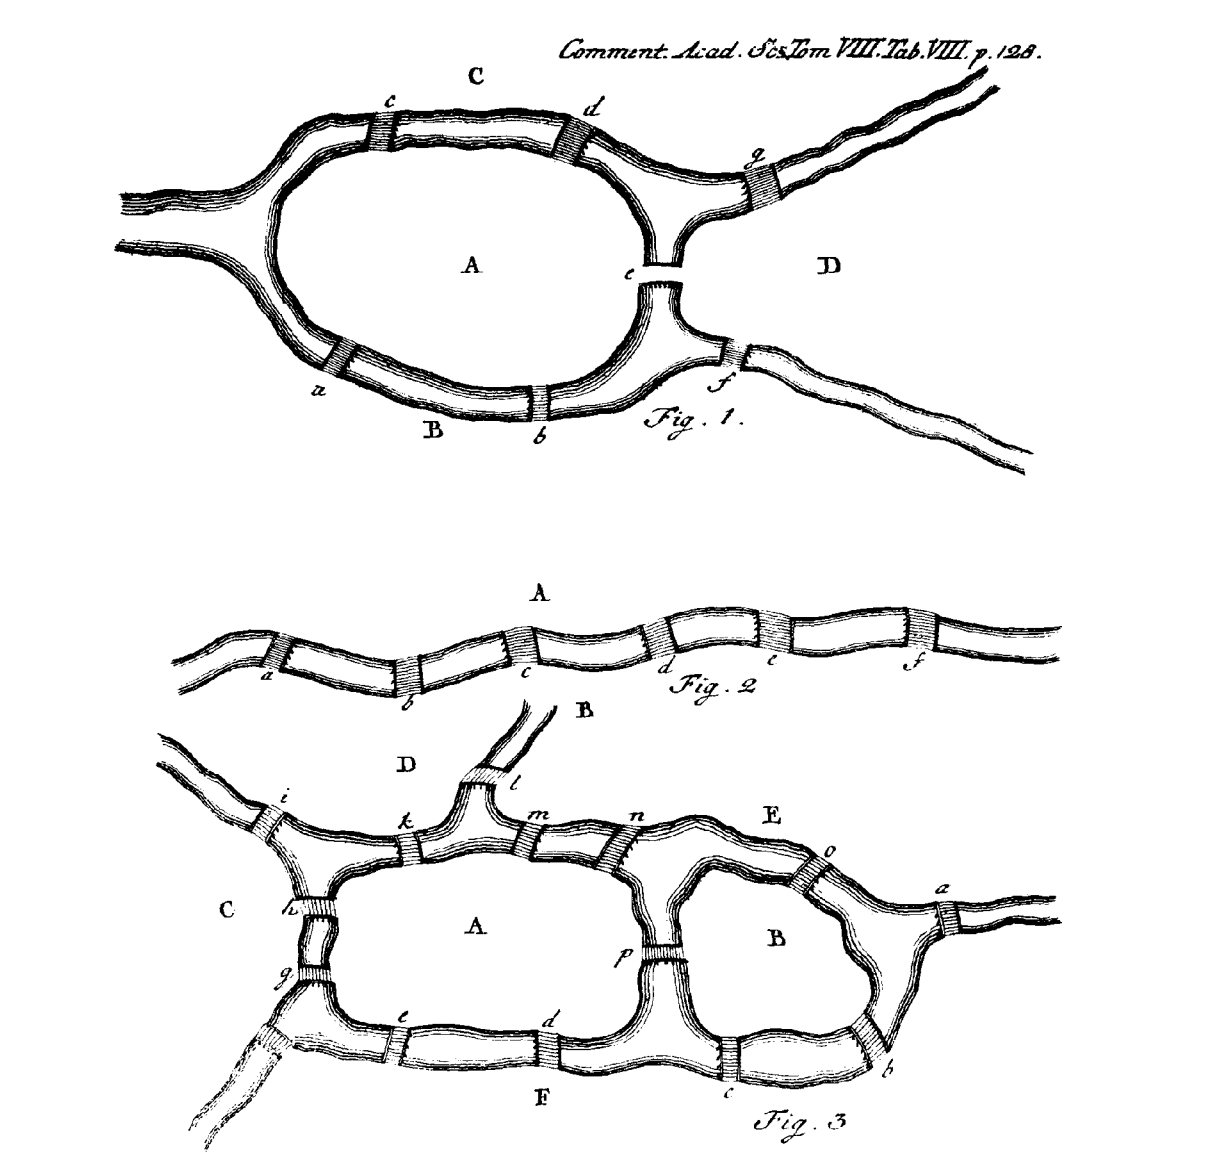
\includegraphics[width=3in]{assets/7bridges-euler.png}
  \caption{Eulers original drawing of the Seven Bridges of Köningsberg} 
  \label{fig:7bridgesEuler}
\end{figure}

%Based on the solution of the ``Seven Bridges of Köningsberg''-problem, Euler presented a theorem. This theorem states that if the graph is planar and connected, and if \textit{v} is the number of vertices, \textit{e} is the number of edges and \textit{f} is the number of faces\footnote{Regions between edges of a plane graph that does not have any edges in it}, then 
%\newline
%\newline
%\centerline{$v-e+f=2$}
%\newline
%\newline
%This theorem demonstrates that if it does not exist a path in the graph that will allow to visit every node using every edge exactly once, the sum will not be 2. An illustration of the bridges in Köningsberg as a graph is presented Figure \vref{fig:7bridgesIllustration} and simplified the illustration in figure \vref{fig:7bridgesSimplification}. The graph consists of 4 vertices, seven edges, and four faces, where the faces are specified with numbers 1-4. If the theorem described above is used, we see that $4-7+4\neq2$, which is consistent with Euler's proof from 1736. 

%\begin{figure}[H]
%  \centering
%  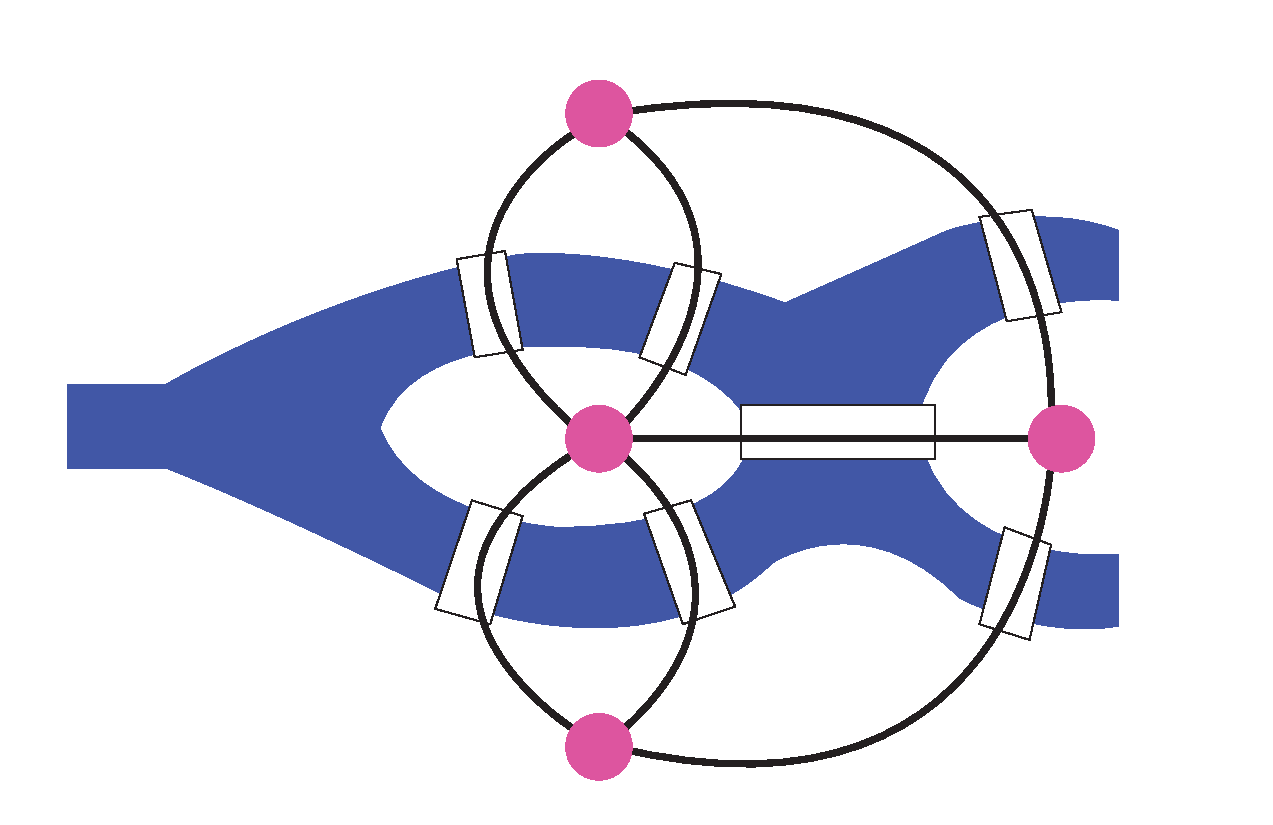
\includegraphics[width=4in]{assets/7bridges.pdf}
%  \caption{Illustration of the Seven Bridges of Köningsberg as a graph}
%  \label{fig:7bridgesIllustration}
%\end{figure}

%\begin{figure}[H]
%  \centering
%  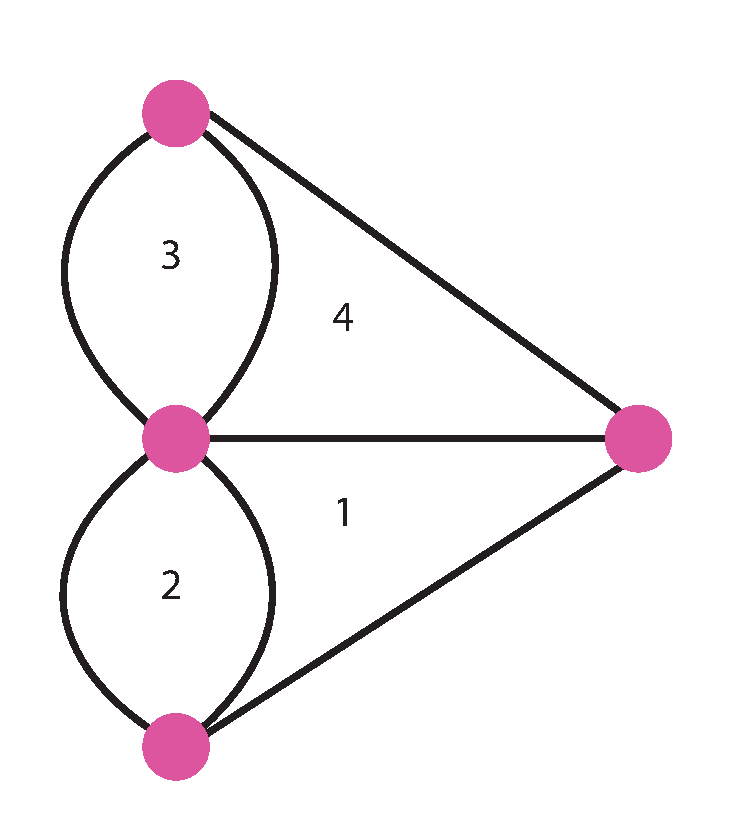
\includegraphics[width=2in]{assets/7bridges2.pdf}
%  \caption{Illustration of the Seven Bridges of Köningsberg as a simplified graph} 
%  \label{fig:7bridgesSimplification}
%\end{figure}

Graph databases use graph structures for semantic queries with nodes, edges, and properties to represent and store data.
The nodes represent entities, such as people, accounts, or bus stops, while the edges represent the relationships, such as ``Friend of'' or ``Belongs to'', between the nodes. A property is relevant information that can relate to either a node or an edge, such as ``Name'' or ``Travel Time''.
%Må omformuleres
Applications of graph databases can include calculating routes and finding the shortest path between locations in a network, such as a road or rail network, airspace network, or logistical network \citep[p.102]{robinson13}. 
%Må omformuleres Compared to relational databases, are graph databases often faster for associative data sets, and map more directly to the structure of object-oriented applications. They can scale more naturally to large data sets as they do not typically require extensive join operations. A drawback to graph databases is the inertia of finding all objects of a specific type.  The following operations are not recommended using graph databases: large, set-oriented wueries, graph global operations and simple, aggregate-oriented queries\citep[p. 40-41]{bruggen14}

\subsection{Neo4j}
\label{subsubsec:neo4j}
Neo4j \citep{website:neo4j} is an open-source graph database, implemented in Java. It is ranked the most popular graph database worldwide \citep{website:graphdbranking} and is used by several large companies such as Telenor \citep{website:telenor}, Walmart \citep{website:walmart} and Cisco \citep{website:cisco}. It is a native graph database optimized and designed for storing and managing graphs and is known for extremely fast traversals of relationship. The underlying data model of Neo4j is the labeled property graph and is one of the most generic and versatile of all graph models\citep[p.73]{robinson13}. This graph data model gives four different fundamental building blocks to structure and store data. These building blocks includes Nodes to store entity information, Relationships to connect nodes to another, Properties for relevant information, and Labels for creating subgraphs.

A query that is extremely well suited for graph databases are queries for finding the paths between different nodes in a graph. Neo4j can be used to see whether a path exists, finding the optimal path, and looking for variability in the path\citep[p. 51]{bruggen14}. Neo4j includes built-in methods for finding the shortest path, including Dijkstra's algorithm. Dijkstra's algorithm \cite[p.658-662]{cormen09} maintains a set $S$ of vertices' whose final shortest-path weights from the source $s$ have already been determined. The algorithm repeatedly selects the vertex $u = V - S$ with the minimum shortest path estimate, adds $u$ to $S$, and relaxes\footnote{Making a change that reduces constraints.} all edges leaving $u$. The running time of Dijkstra's algorithm is $O((V + E)log V)$ and it is guaranteed to find the shortest path\cite[p.~661]{cormen09}. %Dijkstra is one of the best-known algorithms to calculate the shortest weighted path between two points on a graph, using the properties of the edges as a weight or costs. 
The Relationships in a Neo4j database are capable of being of different RelationshipTypes that, among others, enables the built-in Dijkstra to find the shortest path using only specific RelationshipTypes.

%Sweet spot use cases of neo4j: complex, join-intensive queries, path finding queries\citep[p. 51]{bruggen14}. 

%TODO skrive mer her

%Advantages:
%\begin{itemize} 
%\item Flexibility: model, develop and visualize the world as you experience it. Its simply nodes and relationships. 
%\item Performance: Hyper-connectivity at speed. 
%\item Scalability: Scales up and out, supporting tens of billions of nodes and relationships, and hundred of thousands of ACID transactions per seconds. 
%\item Speed: Able to search trough millions of connections per second, with real time queries that stay fast even as your database grows. 
%\end{itemize}

%\begin{itemize}
%\item Native graph database. 
%\item Property graph. 
%\item Made for real time queries. 
%\item Really fast traversals of relations.
%\item Neo4J has an API that supports traversing - finding shortest path - can weight edges, nodes -
%\end{itemize}
%//en korteste vei mellom n og m men max lengde 3
%match p = shortestPath ( (n) - [*...3]--(m)) return p
%(Vekte kanter: Neo44J har et API som støtter traversering, Dijkstras er innebyd ++ som lar deg vekte kanter - hva er raskeste vei ++)

%Neo4J can be used to evaluate routes after the ants have created route sets.
\section{Motivation} 

Trondheim and neighboring municipalities are among the areas with the greatest population growth in Norway \citep{website:miljopakken}. More people means more traffic, and without action will congestion and environmental problems in these urban areas continue to increase every year. 

Private transportation has many advantages for the citizens compared to the public ones. The citizens do not have to wait for a vehicle or change vehicles during a trip, and it is often more convenient. But private transportation has a lot of negative issues, such as traffic jams and increased travel times, which leads to increased air pollution, noise and accidents. 
 
Having efficient public transportation systems can substantially reduce negative effects of the private transportation networks. The public transportation systems is better suited for urban needs, when they can transport more people per time unit than cars, needing much less space. The environment package \citep{website:miljopakken} for transport in Trondheim aims to provide better road networks and public transportation. With this they hope to achieve lower emissions, shorter traffic jams and less traffic noise. An inadequately designed transit network can cause very long waiting times and increase uncertainty in bus arriving time, resulting in less people using the service. Therefore, public transportation systems should be improved by providing better travel services, minimizing the total travel time, and inform the public about them, in order to convince more people to travel with it instead of using their own car.

\citet{website:atb} is responsible for planning the public transport throughout Sør-Trøndelag County, and bus services comprise the major component of the public transportation system here. Bus services also has specific attractive features, such as flexible routes, medium capacity, low cost, easy implementation, flexible fleet size, and use of existing facilities. 
From a meeting with AtB we learned that the current solution of AtB consists of an experience based route network, where transport planners has constructed reasonable bus route networks and schedules entirely manually, following guidelines and exploiting local knowledge. As a result, the efficiency of the resulting networks is dependent of the designers experience and his / hers existing knowledge of constraints and transportation demands. 

The problem of designing the optimal set of routes for a fleet of vehicles, in order to serve a given set of customers, is referred to the vehicle routing problem (VRP). The urban transit network problem(UTNDP) is an example of this broader optimization problem, and is the problem of designing urban transit routes and schedules. The two major components of the UTNDP are the urban transit routing problem(UTRP) and the urban transit scheduling problem (UTSP). UTRP involves the development of efficient transit routes on an existing transit network, with predefined pick-up / drop-off point (e.g bus routes), and UTSP is assigning the schedules for the vehicles. In practice, the two phases are usually implemented sequentially, with the routes determined in advance of the schedules.%Skal denne være med her?

Satisfying all customer needs and in addition keeping all operator costs in check, can be difficult to achieve. Operator costs can include the total number of buses, total bus running distance and the total operating hours. A minimum trip time, amount of transitions, and a not too crowded bus (customers can tolerate standing in 15 minutes ) are among the most important factors that determine the passengers choice of public transit, AtB experiences. 

In the past, transit planners have done reasonable job designing transit networks and schedules without the assistance of scientific tools or systematic procedures, by using their experience and judgment and following established guidelines. Nevertheless, for a really large network it is almost impossible to design an efficient transit route network and bus schedules relying only on past experience and guidelines, because in a large urban area the number of bus routes and bus stops are extremely large. The manual attempts to provide an acceptable solution to the vehicle routing problems are not able to solve these large network problems efficient. In order to overcome this problem, the number of journal publications on vehicle routing problems have increased in recent decades, with the researchers efforts to contribute to the problem.  The increase in researching on these areas is also due to the progress in computational resources, and this has opened new possibilities for modeling more complex routing problems. %These new arising real-world applications provide inspiration for developing new approaches for coordinating complex transportation processes. %Skrives om litt
%In recent years network optimization has become an important field in operational research. Shortest paths, network flows, traffic equilibrium, tsp, vrp, as well as design of an optimal network. Reasons for great interest in network optimization: broad applicability to problemts in pricate entrerprise as well as those in public systems. Networks: changing demands: leads to regurlarly adapted or expanded to meet changing nemands; leads to decision problems than can be supported by network optimization. \citep{mandl79}

%TODO: skrive litt til
Swarm intelligence algorithms has proven to be useful in many vehicle routing problems, and many studies have been done to improve the quality of such problems.
\subsection{Related work}

The related work for this thesis is gathered through a structure literature review. This process is conducted by thoroughly considering what we believe is the most important key words for collecting the most relevant literature concerning our goal, and is properly described in the Experiments and Results-chapter[\ref{experimentsAndResults}], and is entirely explained in the appendix[\ref{appendixA}][\ref{appendixB}]. The literature in this section are the results of the final data synthesis of the structured literature review. \newline

Swarm intelligence algorithms has proven to be useful in many vehicle routing problems, and many studies have been done to improve the quality of such problems. One of the research questions in this thesis is to establish whether it is possible to  solve vehicle routing problems using swarm intelligence and the results of the conducted structured literature will help us establish that. \citet{dorigo97} and \citet{lucic03} are two of the first published papers that confirms this research question by describing methods using swarm intelligence to solve highly complex route optimization problems. The use respectively an ant colony system and a bee system to solve the Traveling Salesman Problem (TSP), which is a subproblem of VRP. 

\citet{hsiao04} presented an optima approach to search for the best path of a map considering the traffic loading conditions. To do this, they proposed an algorithm based on ACO techniques to search for the shortest path from a desired origin to a desired destination. They random-generated a map consisting of 100-500 nodes, and compared their algorithm to a brute method emphasizing on the time used to generate the route. Their results states that if the map consists of more than 200 nodes, the ACO performs better than a brute method. In fact, their results shows that the more nodes the map contains, the higher the benefit of using the ACO algorithm.  

\citet{yang07} presented an optimization model for a bus network design based on the coarse-grain parallel ant colony algorithm (CPACA). CPACA is an optimization algorithm the develops a strategy to update the increased pheromone, called Ant Weight, where the path searching activities of the ants are adjusted based on the objective function. The model aims to minimize the average trip time by maximizing the number of direct travelers per unit length. Their results are compared with the classical MAX-MIN ant system (MMAS)\citep{stutzle99} and with ACA with Ant-weight strategy (ACA+). The comparison shows that CPACA performs better regarding both average direct traveler density and run time. They concluded that suitable future research will be to improve the searching efficiency, because their simulation shows that their algorithms is more stable and the runtime is more satisfactory when the number of nodes are less than 1000. 

\citet{salehi-nezhad07} presented an algorithm to search for the best direction between two desired origin and destination intersections in cities, called Ant-based Vehicle Navigation algorithm. The algorithm was applied on a part of the city of \textit{Kerman}, and the results are encouraging. The algorithm provides a fast access, low cost and easy method for vehicle navigation in cities without assisting GPS.

\citet{tripathi09} solved the vehicle routing problem with stochastic demand, in which the customer demand is modeled as a stochastic variable. They performed this using an improved version of the ACO approach, called ns-AAA SO, which oriented the search progressively towards favoring the global optimal solution. The characteristics and search capability of ns-AAA SO was then compared with both a standard ACO algorithm and a genetic algorithm. The results shows that ns-AAA SO outperforms the other two algorithms in every problem instance described by the authors. 

\citet{salehinejad10} introduced a route selection system which uses an ant colony system to detect an optimum multiparameter direction between two desired points in urban areas. The system employs fuzzy logic for local pheromone updating, and the proposed algorithm is called Fuzzy Logic-Ant Colony System (FLACS). The algorithm is applied to a part of London, United Kingdom, consisting of 42 junctions (nodes). The FLACS algorithm is compared to a standard ACS-algorithm and a $A^*$-ACS-algorithm emphasizing on the parameters ``distance'', ``traffic'' and ``incident risk'', which is said to be important to travelers. The presented results are the average of 10 randomly selected O/D pairs, and their result graphs states that FLACS performs better at average than both the standard ACS and the $A^*$-ACS regarding operational cost. The performance is independent of the importance rate of the parameters mentioned above. It is, however, worth mentioning that the estimation of further traffic data is done by ANNs, and therefore the traffic data used for each algorithm is not exactly the same. FLACS has less running time than $A^*$-ACS, but more than the standard ACS due to its Fuzzy Logic system component. 

\citet{jiang10} describes an improved ACO (IACO) algorithm to solve the Urban Transit Network Optimization which is described as a typical nonlinear combinatorial optimization problem. Improvements to the algorithm includes a stagnation counter to determine if an ant had stagnated and adding of extra pheromone intensity to newly discovered paths. This is done to compensate for the classical ACOs shortcomings of easily falling into stagnation and therefore obtain a local optimal solution. The IACO algorithm is, like the algorithm described by \citet{yang07}, compared to the classical MMAS algorithm. The results shows significant improvement to the convergence speed compared to MMAS. The average number of iterations to find the optimal solution was reduced from 1060 using MMAS to 548 using IACO. The average path distance was shortened from 15554.74 using MMAS to 15509.02 using IACO.  

\citet{poorzahedy11} proposed an Ant System application for solving the bus network design problem. The bus network design problem is a problem that is usually decomposed into two problems, respectively network configuration and bus frequency determination. Some of the characteristics of the authors algorithm is that it works with a decision graph, rather than on the bus network it self. The algorithm is only concerned about one objective; a combination of travel time for the users and the bus fleet size for the operator. The application was used to design the bus network of Mashhad, a city with a population of over 2 millions, and further compared with a genetic algorithm (GA). Their results shows that their algorithm performs better than the GA in both the number of routes, fleet size, in-vehicle travel time and waiting time. GA performs better than the Ant System algorithm with respect to travelers walking time. 

\citet{dias14} introduced an inverted ACO (IACO) algorithm. The idea was that the IACO algorithm inverts the classical ACO logic by converting the attraction of ants towards pheromones into a repulsion effect. The IACO was then used in a decentralized traffic management system, where the drivers acts as the inverted ants. The ideas was that drivers are repelled by the scent of pheromones (other drivers), and the system thus avoids congested roads. The IACO algorithm described, was compared to a shortest-time algorithm (ST). The IACO algorithm performs better than the ST algorithm, with the respect to trip time, travel length, fuel consumption and $CO_2$ emissions. This is as long as a considerable amount (25-50\%, depending on whether it was tested on a radial and ring network or a lattice network) of the vehicles uses an algorithm to decide which road to choose. 

\citet{nikolic14} proposed a model for the transit network design problem. To do this they used an approach based on BCO metaheuristic. They considered the network design problem in a way that the algorithm decided the links that was included in the transit network, and further creating designed bus routes based on the links. They tested two orders of importance of the objective functions (an order that is best for passengers and an order that is best for the transit operator). The algorithm was tested on Mandl's benchmark problem of a Swiss bus network\citep{mandl80}. This is probably the only widely investigated and accepted benchmark problem in the relevant literature\citep{kechagiopoulos14}. Their algorithm was compared to other competitive approaches (\citet{mandl80}; \citet{shih94}; \citet{baaj95}; \citet{bagloee11}), and the results may be considered as ambiguous. The algorithm proposed by \citet{nikolic14} performed best regarding travel time and number for transfers, but was sometimes outperformed regarding in-vehicle time and out-of-vehicle time. 

\citet{sedighpour14} introduced a hybrid ACO (HACO) algorithm where they used a new state transition rule and a candidate list, as well as several local search techniques and a new pheromone update rule. The hybrid was designed to overcome some of the original ACOs shortcomings, such as slow computing speed and local convergence. The HACO algorithm was applied to the open vehicle routing problem, a variant of the vehicle routing problem in which vehicles are not required to return to the depot after completing a service. The HACO algorithm was compared with three versions of PSO (standard PSO, PSO without one-point move (PSOWO) and PSO without neighbors (PSOWN). The algorithms were tested on fifteen different sets, consisting of 19 to 72 nodes with 2 to 7 vehicles fixed at the minimum possible. Their result table showed that HACO found the optimal solution in 14 out of 15 set compared to PSO with 13/15, PSOWO with 0/15 and PSOWN with 9/15. In the one set HACO did not find an optimal solution it still performed better than the other algorithms. As mentioned above, HACO was designed to overcome some of the original ACOs shortcomings and we therefore believe it is worth mentioning that the algorithm was not actually compared to the original ACO algorithm. 

\citet{kechagiopoulos14} designed and presented an optimization algorithm based on PSO. Their goal was to find an efficient solution to the urban transit routing problem (UTRP), which is a NP-hard problem that deals with the construction of route networks for public transportation. The target problem was Mandl's benchmark problem. Their algorithm is compared with competitive approaches (including genetic algorithms and other metaheuristic approaches) mentioned in literature (\citet{baaj91}; \citet{chakroborty02}; \citet{kidwai98}; \citet{fan10}; \citet{fan09-2}; \citet{zhang10}; \citet{chew12}). The algorithms are compared with regard to the percentage of total transfer demands satisfied directly ($d_0$), with one transfer ($d_1$), two transfers ($d_2$), or with more than two transfers or not satisfied at all ($d_{unsat}$). The algorithms are also compared regarding average in-vehicle travel time ($ATT$). The experiments are conducted on route set designs with four, six, seven and eight routes. The proposed algorithm performs better than the competitors regarding $ATT$ independent the route size, and achieves a better percentage of direct travelers ($d_0$) except from when the route size is four. The percentage of passengers with more than two transfers or not satisfied at all ($d_{unsat}$), is $0.00$ for all the described algorithms independent of route size. \newline

Based on the described literature we can conclude that swarm intelligence-algorithms shows great promise in solving different vehicle routing problems. We specifically notice that SI-algorithms performs equal and sometimes better than genetic algorithms and  metaheurstic approaches like Simulated Annealing. We also notice that 2 out of the 12 described papers uses Mandl's benchmark problem as a test case for their proposed algorithm, and that 2 out of 12 papers compare their algorithm to \citet{stutzle99}s MAX-MIN ant system (MMAS). It is worth mentioning that none of the proposed algorithms performs optimally in every situation and that there is no consensus in which algorithm is the overall best. It is therefore difficult to draw a singular conclusion to what is the state of the art regarding swarm intelligence and vehicle routing problems. We suggest that a general state of the art regarding the algorithm may be described as being inspired by the way different swarms act in nature, and to further add artificial features to the individuals to optimize for certain objectives. Mandl's benchmark problem was used by 2 out of the 4 papers in our literature review published in 2014, and we therefore believe that using this benchmark problem as a test case may be considered as the state of the art.


%Skrive om at det "To the best of our knowledge" ikke eksisterer en supersverm algoritme. 

\subsection{Mandls Benchmark Problem}
%TODO: kjøpe/leie Mandl boka
%TODO: skrive om 
%Since there is not done any op
In the current research on the VRPs and SI, there are some benchmark data that are available for researchers to use for comparison.... However (as mentioned in RW), for the UTNDP problem, Mandls network seems to be the only benchmark instance used by researchers. The road network is a real Swiss road network comprising of 15 nodes and 21 connections between them. And has been thoroughly examined by many optimization approaches such as \citep{kechagiopoulos14}, \citep{fan09}, \citep{nikolic14}. %This makes it easy to measure the performance of your solution. 

%TODO: skrive om 
Christoph Mandl concentrated mainly on the UTRP, and developed a solution in two stages. First, a feasible set of

Christoph Mandl[] approaches the UTNDP problem in a generic form. Mandl concentrated on the UTRP, and developed a solution in two stages. First, a feasible set of routes was generated, and then heuristics were applied to improve the quality of the initial route set / tour plan. The route generation phase involved computing the shortest path between all sets of vertices's using Dijstras[], and then producing the route set with the shortest paths that contained the most nodes, respecting the positions of any nodes selected as terminals. Nodes not selected, were iteratively included into routes, or new routes were created with unserved nodes as route terminals. In the first phase, Mandl only considered in-vehicle travel costs when accessing route quality. He then suggested an initial route set, and used these in the second phase. The second phase included obtaining the new routes at an intersection node, including a node that was close to a route (if travel demand between this node and the node on the route was high), and / or excluded a node from a route set that was already served by another rote (if the travel demand between this node and the other nodes in the route was low). Waiting costs were also considered in the second phase, in addition to in-vehicle travel costs. Waiting times were fixed as constant values, according to specified vehicle frequencies. 

%IFylles inn i results: in order to demonstrate the efficiency and the effectiveness of our algorithm... the Swiss road network introduced by Mandl is used. This road network has been already used as a benchmark problem by many researchers in the literature. \citep{kechagiopoulos14}


\subsection{Graph Database}
\textit{Denne er foreløpig kopiert fra Wikipedia}
%Skrives om
\par
A graph database is a database that uses graph structures for semantic queries with nodes, edges, and properties to represent and store data. A graph database is any storage system that provides index-free adjacency.This means that every element contains a direct pointer to its adjacent elements and no index lookups are necessary. General graph databases that can store any graph are distinct from specialized graph databases such as triplestores and network databases.
%Skrives om
Graph databases are based on graph theory. Graph databases employ nodes, properties, and edges. Nodes represent entities such as people, businesses, accounts, or any other item you might want to keep track of. Properties are pertinent information that relate to nodes. Edges are the lines that connect nodes to nodes or nodes to properties and they represent the relationship between the two. Most of the important information is really stored in the edges. Meaningful patterns emerge when one examines the connections and interconnections of nodes, properties, and edges.

Compared with relational databases, graph databases are often faster for associative data sets[citation needed], and map more directly to the structure of object-oriented applications. They can scale more naturally to large data sets as they do not typically require expensive join operations. As they depend less on a rigid schema, they are more suitable to manage ad hoc and changing data with evolving schema's. Conversely, relational databases are typically faster at performing the same operation on large numbers of data elements.
Graph databases are a powerful tool for graph-like queries, for example computing the shortest path between two nodes in the graph. Other graph-like queries can be performed over a graph database in a natural way (for example graph's diameter computations or community detection).

\subsubsection{Neo4J}
Neo4J is a native graph database, and is a success way to store a transport graph [Reference]. It is known for extremely fast traversals of relationships. Neo4J can be easily constructed to a transit network. It is fast finding shortest path (by Dijkstra's algorithm), and it is easy to change the database via the REST API. 
Neo4J is a highly scalable open source graph database that supports ACID, has high-availability clustering for enterprise deployments, and comes with a web-based administration tool that includes full transaction support and visual node-link graph explorer. Neo4j is accessible from most programming languages using its built-in REST web API interface. Neo4j is the most popular graph database in use today.[10]


%\begin{itemize}
%\item Native graph database. 
%\item Property graph. 
%\item Made for real time queries. 
%\item Really fast traversals of relations.
%\item Neo4J has an API that supports traversing - finding shortest path - can weight edges, nodes -
%\end{itemize}
%//en korteste vei mellom n og m men max lengde 3
%match p = shortestPath ( (n) - [*...3]--(m)) return p
%(Vekte kanter: Neo44J har et API som støtter traversering, Dijkstras er innebyd ++ som lar deg vekte kanter - hva er raskeste vei ++)

%Neo4J can be used to evaluate routes after the ants have created route sets.
\subsection{Problem Statement}
%TODO: skrive hva vi skal gjøre
Through our review of research, we note that there have been no research that aims to combine attributes from different swarm intelligence methods to improve the optimization process. For this reason, we will in this thesis investigate the possibility to combine some of the best attributes from ACO and BCO in order to achieve better results regarding route optimization.

After a meeting with AtB we learned that AtB does not have accurate data about the travel demand, and that there has not been done any attempts to optimize their transit network with computational resources. Accurate estimates of travel demand are essential as they are an important factor for the algorithm. A good tour plan will ensure that travel requirements with a heavy demand are satisfied, with short travel times and few vehicle transfers. 

We are highly motivated on the development of an algorithm and we want to focus our research on the development of a new algorithm, rather than on gathering data to determine the travel demands of the bus network of Trondheim. In order to demonstrate the efficiency and the effectiveness of our algorithm we will compare our results with Mandls benchmark data. Mandls benchmark problem includes %TODO: FYLL INN SUS%
As mentioned, this road network has already been used as a benchmark problem by many researchers in the literature. We believe that a comparison of our algorithm to others described in literature, will be important to establish both the efficiency and the effectiveness of our algorithm. This comparison will be enabled using Mandls network. Our aim is to create a general solution, where we hope to achieve better results than the ones we are comparing it with, and that this in the future can be used to optimize AtBs transit network. 

We will focus our research on the urban transit routing problem, to make the routes more convenient both concerning customers and operators. The objectives we want to focus on is satisfying the customers and in addition keeping the operator costs in check. Trough our research we have found that 
\begin{itemize}
\item Minimum number of transfers
\item Minimum in-vehicle time
\end{itemize}
is important factors for determine the customers satisfaction ({\citet{kechagiopoulos14}; \citet{dias14}, \citet{yang07} }). There has also been done a lot of research on these areas, and therefore data is available so we can compare our results against this. This factors will also lead to minimum total travel time. 
\par
Minimum fleet size and better departures will implicitly ..
\par
Based on these new routes, we can hopefully draw conclusions....


  



\chapter{Preparatory Research}
\label{relatedWork}
\subsection{Related work}

The related work for this thesis is gathered through a structure literature review. This process is conducted by thoroughly considering what we believe is the most important key words for collecting the most relevant literature concerning our goal, and is properly described in the Experiments and Results-chapter[\ref{experimentsAndResults}], and is entirely explained in the appendix[\ref{appendixA}][\ref{appendixB}]. The literature in this section are the results of the final data synthesis of the structured literature review. \newline

Swarm intelligence algorithms has proven to be useful in many vehicle routing problems, and many studies have been done to improve the quality of such problems. One of the research questions in this thesis is to establish whether it is possible to  solve vehicle routing problems using swarm intelligence and the results of the conducted structured literature will help us establish that. \citet{dorigo97} and \citet{lucic03} are two of the first published papers that confirms this research question by describing methods using swarm intelligence to solve highly complex route optimization problems. The use respectively an ant colony system and a bee system to solve the Traveling Salesman Problem (TSP), which is a subproblem of VRP. 

\citet{hsiao04} presented an optima approach to search for the best path of a map considering the traffic loading conditions. To do this, they proposed an algorithm based on ACO techniques to search for the shortest path from a desired origin to a desired destination. They random-generated a map consisting of 100-500 nodes, and compared their algorithm to a brute method emphasizing on the time used to generate the route. Their results states that if the map consists of more than 200 nodes, the ACO performs better than a brute method. In fact, their results shows that the more nodes the map contains, the higher the benefit of using the ACO algorithm.  

\citet{yang07} presented an optimization model for a bus network design based on the coarse-grain parallel ant colony algorithm (CPACA). CPACA is an optimization algorithm the develops a strategy to update the increased pheromone, called Ant Weight, where the path searching activities of the ants are adjusted based on the objective function. The model aims to minimize the average trip time by maximizing the number of direct travelers per unit length. Their results are compared with the classical MAX-MIN ant system (MMAS)\citep{stutzle99} and with ACA with Ant-weight strategy (ACA+). The comparison shows that CPACA performs better regarding both average direct traveler density and run time. They concluded that suitable future research will be to improve the searching efficiency, because their simulation shows that their algorithms is more stable and the runtime is more satisfactory when the number of nodes are less than 1000. 

\citet{salehi-nezhad07} presented an algorithm to search for the best direction between two desired origin and destination intersections in cities, called Ant-based Vehicle Navigation algorithm. The algorithm was applied on a part of the city of \textit{Kerman}, and the results are encouraging. The algorithm provides a fast access, low cost and easy method for vehicle navigation in cities without assisting GPS.

\citet{tripathi09} solved the vehicle routing problem with stochastic demand, in which the customer demand is modeled as a stochastic variable. They performed this using an improved version of the ACO approach, called ns-AAA SO, which oriented the search progressively towards favoring the global optimal solution. The characteristics and search capability of ns-AAA SO was then compared with both a standard ACO algorithm and a genetic algorithm. The results shows that ns-AAA SO outperforms the other two algorithms in every problem instance described by the authors. 

\citet{salehinejad10} introduced a route selection system which uses an ant colony system to detect an optimum multiparameter direction between two desired points in urban areas. The system employs fuzzy logic for local pheromone updating, and the proposed algorithm is called Fuzzy Logic-Ant Colony System (FLACS). The algorithm is applied to a part of London, United Kingdom, consisting of 42 junctions (nodes). The FLACS algorithm is compared to a standard ACS-algorithm and a $A^*$-ACS-algorithm emphasizing on the parameters ``distance'', ``traffic'' and ``incident risk'', which is said to be important to travelers. The presented results are the average of 10 randomly selected O/D pairs, and their result graphs states that FLACS performs better at average than both the standard ACS and the $A^*$-ACS regarding operational cost. The performance is independent of the importance rate of the parameters mentioned above. It is, however, worth mentioning that the estimation of further traffic data is done by ANNs, and therefore the traffic data used for each algorithm is not exactly the same. FLACS has less running time than $A^*$-ACS, but more than the standard ACS due to its Fuzzy Logic system component. 

\citet{jiang10} describes an improved ACO (IACO) algorithm to solve the Urban Transit Network Optimization which is described as a typical nonlinear combinatorial optimization problem. Improvements to the algorithm includes a stagnation counter to determine if an ant had stagnated and adding of extra pheromone intensity to newly discovered paths. This is done to compensate for the classical ACOs shortcomings of easily falling into stagnation and therefore obtain a local optimal solution. The IACO algorithm is, like the algorithm described by \citet{yang07}, compared to the classical MMAS algorithm. The results shows significant improvement to the convergence speed compared to MMAS. The average number of iterations to find the optimal solution was reduced from 1060 using MMAS to 548 using IACO. The average path distance was shortened from 15554.74 using MMAS to 15509.02 using IACO.  

\citet{poorzahedy11} proposed an Ant System application for solving the bus network design problem. The bus network design problem is a problem that is usually decomposed into two problems, respectively network configuration and bus frequency determination. Some of the characteristics of the authors algorithm is that it works with a decision graph, rather than on the bus network it self. The algorithm is only concerned about one objective; a combination of travel time for the users and the bus fleet size for the operator. The application was used to design the bus network of Mashhad, a city with a population of over 2 millions, and further compared with a genetic algorithm (GA). Their results shows that their algorithm performs better than the GA in both the number of routes, fleet size, in-vehicle travel time and waiting time. GA performs better than the Ant System algorithm with respect to travelers walking time. 

\citet{dias14} introduced an inverted ACO (IACO) algorithm. The idea was that the IACO algorithm inverts the classical ACO logic by converting the attraction of ants towards pheromones into a repulsion effect. The IACO was then used in a decentralized traffic management system, where the drivers acts as the inverted ants. The ideas was that drivers are repelled by the scent of pheromones (other drivers), and the system thus avoids congested roads. The IACO algorithm described, was compared to a shortest-time algorithm (ST). The IACO algorithm performs better than the ST algorithm, with the respect to trip time, travel length, fuel consumption and $CO_2$ emissions. This is as long as a considerable amount (25-50\%, depending on whether it was tested on a radial and ring network or a lattice network) of the vehicles uses an algorithm to decide which road to choose. 

\citet{nikolic14} proposed a model for the transit network design problem. To do this they used an approach based on BCO metaheuristic. They considered the network design problem in a way that the algorithm decided the links that was included in the transit network, and further creating designed bus routes based on the links. They tested two orders of importance of the objective functions (an order that is best for passengers and an order that is best for the transit operator). The algorithm was tested on Mandl's benchmark problem of a Swiss bus network\citep{mandl80}. This is probably the only widely investigated and accepted benchmark problem in the relevant literature\citep{kechagiopoulos14}. Their algorithm was compared to other competitive approaches (\citet{mandl80}; \citet{shih94}; \citet{baaj95}; \citet{bagloee11}), and the results may be considered as ambiguous. The algorithm proposed by \citet{nikolic14} performed best regarding travel time and number for transfers, but was sometimes outperformed regarding in-vehicle time and out-of-vehicle time. 

\citet{sedighpour14} introduced a hybrid ACO (HACO) algorithm where they used a new state transition rule and a candidate list, as well as several local search techniques and a new pheromone update rule. The hybrid was designed to overcome some of the original ACOs shortcomings, such as slow computing speed and local convergence. The HACO algorithm was applied to the open vehicle routing problem, a variant of the vehicle routing problem in which vehicles are not required to return to the depot after completing a service. The HACO algorithm was compared with three versions of PSO (standard PSO, PSO without one-point move (PSOWO) and PSO without neighbors (PSOWN). The algorithms were tested on fifteen different sets, consisting of 19 to 72 nodes with 2 to 7 vehicles fixed at the minimum possible. Their result table showed that HACO found the optimal solution in 14 out of 15 set compared to PSO with 13/15, PSOWO with 0/15 and PSOWN with 9/15. In the one set HACO did not find an optimal solution it still performed better than the other algorithms. As mentioned above, HACO was designed to overcome some of the original ACOs shortcomings and we therefore believe it is worth mentioning that the algorithm was not actually compared to the original ACO algorithm. 

\citet{kechagiopoulos14} designed and presented an optimization algorithm based on PSO. Their goal was to find an efficient solution to the urban transit routing problem (UTRP), which is a NP-hard problem that deals with the construction of route networks for public transportation. The target problem was Mandl's benchmark problem. Their algorithm is compared with competitive approaches (including genetic algorithms and other metaheuristic approaches) mentioned in literature (\citet{baaj91}; \citet{chakroborty02}; \citet{kidwai98}; \citet{fan10}; \citet{fan09-2}; \citet{zhang10}; \citet{chew12}). The algorithms are compared with regard to the percentage of total transfer demands satisfied directly ($d_0$), with one transfer ($d_1$), two transfers ($d_2$), or with more than two transfers or not satisfied at all ($d_{unsat}$). The algorithms are also compared regarding average in-vehicle travel time ($ATT$). The experiments are conducted on route set designs with four, six, seven and eight routes. The proposed algorithm performs better than the competitors regarding $ATT$ independent the route size, and achieves a better percentage of direct travelers ($d_0$) except from when the route size is four. The percentage of passengers with more than two transfers or not satisfied at all ($d_{unsat}$), is $0.00$ for all the described algorithms independent of route size. \newline

Based on the described literature we can conclude that swarm intelligence-algorithms shows great promise in solving different vehicle routing problems. We specifically notice that SI-algorithms performs equal and sometimes better than genetic algorithms and  metaheurstic approaches like Simulated Annealing. We also notice that 2 out of the 12 described papers uses Mandl's benchmark problem as a test case for their proposed algorithm, and that 2 out of 12 papers compare their algorithm to \citet{stutzle99}s MAX-MIN ant system (MMAS). It is worth mentioning that none of the proposed algorithms performs optimally in every situation and that there is no consensus in which algorithm is the overall best. It is therefore difficult to draw a singular conclusion to what is the state of the art regarding swarm intelligence and vehicle routing problems. We suggest that a general state of the art regarding the algorithm may be described as being inspired by the way different swarms act in nature, and to further add artificial features to the individuals to optimize for certain objectives. Mandl's benchmark problem was used by 2 out of the 4 papers in our literature review published in 2014, and we therefore believe that using this benchmark problem as a test case may be considered as the state of the art.


%Skrive om at det "To the best of our knowledge" ikke eksisterer en supersverm algoritme. 

\section{Structured Literature Review}
\label{sec:structuredLiteratureReview}

\citet{cohen88} introduced a five-stage model for evaluating research in terms of a five-stage cycle, where the first stage involves refining the research topic to a task, and identifying a view of how to accomplish the task. Our task / goal in this research is, hopefully, contributing to producing effective urban transit routes to Trondheim by using swarm intelligence methods. This is interesting because congestion and environmental problems in Trondheim is increasing every year due to the population growth\citep{website:miljopakken}. Efficient public transportation systems can help achieve lower emissions, less traffic jams and traffic noise, and when AtB's\citet{website:atb} current solution consist of an experience based route network, it may not be an acceptable and optimal solution to the public transportation system. The motivation behind swarm intelligence is, as slightly initiated in Section \vref{sec:motivation}, the proof of ability in solving vehicle routing problems. 

To establish whether the research topic has been studied before and what the state-of-the art on these problems are, we conducted a Structured Literature Review based on the model suggested by \citet{kofod2014}. As stated in \citep{kofod2014} synthesizing available information before tackling an area of research can, for example, help mapping out existing solutions, avoid duplicating the effort, and highlight areas where additional research is required. Section \vref{sec:SLRprocessDescribtion} is a summary of the conducted literature review, and the complete review can be found in Appendix \vref{appendixA} and Appendix \vref{appendixB}. 

 %We also believe that a graph database can have benefits we can take advantage of in solving our problem, and therefore wanted to investigate what might have been done before on this research area.

\subsection{Process Description}
\label{sec:SLRprocessDescribtion}

Our research topic was formed into a problem. The problem and the following research questions can be found in Appendix \ref{appendixA}, Section \vref{sec:researchQSLR}.

The list of sources for retrieving relevant literature to our defined research questions, were selected based on \citep[p.3]{kofod2014}, and can be found in Appendix \vref{appendixB}. 

Key search terms was decided based on our problem, formed into groups of synonyms, and assembled into a complete search term. The key search terms and the complete search term can be found in appendix \ref{appendixA}, section \vref{searchterm} and section \vref{sec:searchTerms}, respectively.

To exclude irrelevant literature, some Inclusion Criteria was decided to ensure a level of relevance. The Inclusion Criteria can be found in Appendix \ref{appendixA}, Section \vref{sec:inclusionCriteria}. After the Inclusion Criteria filtering, we had 42 sources for the related literature, including scientific papers and master theses. 

Quality Criteria was determined to ensure quality in the final papers and to filter away studies not theoretically relevant for our thesis. Each of the studies under consideration was classified according to the Quality Criteria, by scoring the papers on each Quality Criteria. Each point was given a score, where 1 point denote relevant, $\frac{1}{2}$ point denote partly relevant and 0 points denote not relevant. For retrieving the most relevant papers based on the content and not just the quality of the paper, Quality Criteria \ref{itm:qa1a} and \vref{itm:qa1b} was multiplied by 3. Quality Criteria \ref{itm:qa1a} is concerned about whether or not the research in fact is a Vehicle Routing Problem and Quality Criteria \ref{itm:qa1b} addresses whether or not swarm intelligence is the main optimization method. 

Table \vref{table:literature} shows the papers that were selected based on the Inclusion Criteria and the scores given based on Quality Criteria.

The average score of the read literature was 13.01 $\approx$ 13, and literature given a score $\geq{1.5}$ above average were selected. This resulted in 12 final researches, which can be seen in Table \vref{table:finalliterature}. These researches will form the foundation of our thesis, and Section \vref{sec:relatedWork} describes and summarizes the selected literature, referred to as the related work. 

\section{Related Work} 

Our first research question can be summed up to what has been done before regarding solving VRP's using swarm intelligence. To answer this research question and its subquestions we therefor conducted a structured literature review, which we believe will help us answer these questions. The process of the structured literature review is performed by thoroughly considering what we believe are the most important key words for collecting the most relevant literature, concerning our goal and research questions and using these keywords to search for articles in different search engines. The conducted process is described in the Experiments and Results-chapter[\ref{experimentsAndResults}], and is entirely explained in the appendix[\ref{appendixA}][\ref{appendixB}]. The literature in this section are the results of the final data synthesis of the structured literature review. They all describes a vehicle routing problem solved by a swarm inspired method. \newline

Swarm intelligence algorithms has proven to be useful in many vehicle routing problems, and many studies have been conducted to improve the solution, both regarding time complexity and quality, of such problems. \citet{dorigo97} and \citet{lucic03} were two of the first published papers that shows that methods from swarm intelligence is suitable for solving VRP's. They use respectively an ant colony system and a bee system to solve the Traveling Salesman Problem (TSP), which is a subproblem of VRP. 

Many computer scientists has since then studied the possibility of solving VRPs using swarm intelligence. \citet{hsiao04}, \citet{salehi-nezhad07}, \citet{tripathi09}, \citet{dias14}, and \citet{sedighpour14} all studied the possibility of using swarm intelligence to solve vehicle routing problems involving cars transporting either persons or goods. 

%Mangler informasjon om algoritmene som sammenlignes med. Parametersettingen er beskrevet, men ikke forklart. 
\citet{hsiao04} presented an approach to search for the best path of a map considering the traffic loading conditions. To do this, they proposed an ACO algorithm to search for the shortest path from a desired origin to a desired destination. The presented algorithm is a classic ACO algorithm without changes. To test their algorithm, the random-generated a map consisting of 100-500 nodes, and compared their algorithm to a brute method emphasizing on the time used to generate the route. Their results states that if the map consists of more than 200 nodes, the ACO performs better than a brute method. In fact, they found that the more nodes the map contains, the higher the benefit of using the ACO algorithm. 

%Sammenligner egentlig ikke mot en dritt? Algoritmen er bare testet på et veldig lite testsett. Eksperimentene for å finne parameterne er ikke nevnt, men de brukte parameterne er
\citet{salehi-nezhad07} presented an ant algorithm to search for the best path between two desired origin and destination intersections in cities, called Ant-based Vehicle Navigation algorithm. To get more accurate results than the classic ant algorithms they employed an \textit{awarding/punishment}-method, were the path found by the ``best ants'' are given more pheromone than the path of the ``bad ants''. In order to find the best path, the presented algorithm is concerned about the parameters \textit{distance}, \textit{width}, \textit{traffic load}, \textit{road risk}, \textit{road quality}, and \textit{number of intersections}. The importance of each of the parameters are weighted from 0 to 1 by the user. 

%Mangler informasjon om algoritmene som sammenlignes med
\citet{tripathi09} solved the vehicle routing problem with stochastic demand, in which the customer demand is modeled as a stochastic variable. They performed this using an improved version of the ACO approach, called ns-AAA SO. The proposed algorithm orients the search progressively towards favoring the global optimal solution. To do this they defines that a complete iteration consists of two tours: The first tour is a social tour that corresponds to a standard ACO iteration. The second tour is a neighborhood tour where the ants are allowed to communicate important information found in the social tour and change their solutions. If the fitness value of the new solution is better, the old solution found in the social tour is replaced. To favor the optimal solution, the path of the global best path is given more pheromones. Further, to prevent the search for from entrapment into a local optima, a minimum quantity of pheromone on any edge, $t_{min}$, is always maintained. The performance of ns-AAA SO was compared with both a standard ACO algorithm and a genetic algorithm. They found that ns-AAA SO outperforms the other two algorithms in every problem instance described by the authors.

%Mandler informasjon om parametersetting
\citet{dias14} introduced an inverted ACO (IACO) algorithm. The idea is that the IACO algorithm inverts the logic of the classical ACO algorithm by converting the attraction of ants towards pheromones into a repulsion effect. The proposed approach was used in a decentralized traffic management system, where the drivers acted as the inverted ants. The drivers were repelled by the scent of pheromones (other drivers), and the system thus avoids congested roads. The described approach was compared to a shortest-time algorithm (ST), and the IACO algorithm performs better than the ST algorithm with the respect to trip time, travel length, fuel consumption and $CO_2$ emissions. This is as long as a considerable amount (25-50\%) of the vehicles uses the inverted ant algorithm to decide which road to choose. 

%Sammenligner ikke algoritmen mot original ACO, selvom de sier at de ønsker å forbedre ACO i introduksjonen
\citet{sedighpour14} introduced a hybrid ACO (HACO) algorithm to solve the open vehicle routing problem (OVRP). This is a sub problem of the classical VRP where the vehicles are not required to return to the depot. To overcome some of the shortcomings, such as slow computing speed and local convergence, of the original ACO algorithm they made three major improvements. First they equipped each node with a candidate list containing nodes nearby that had not yet been visited. Second, at each iteration, they applied several local search techniques to the \textit{n} best solutions found to improve them further. Third, they decided the amount of released pheromone based on the rank of the best known solution found so far. The HACO algorithm was compared with three versions of PSO (standard PSO, PSO without one-point move (PSOWO) and PSO without neighbors (PSOWN) regarding performance. The algorithms were tested on fifteen different sets, consisting of 19 to 72 nodes with 2 to 7 vehicles fixed at the minimum possible. Their result table shows that HACO performs better than the others regardless of the test case used.\newline

Urban Transit Network Design Problem (UTRP), a subproblem of VRP, considers other objectives and requires other methods for solving than classical VRP problems. \citet{yang07}, \citet{salehinejad10}, \citet{jiang10}, \citet{poorzahedy11}, \citet{nikolic14}, and \citet{kechagiopoulos14} all addressed problems related to urban transit networks. \newline

%Parameterne er nevnt og den sammenligner med relevante algoritmer
\citet{yang07} presented an optimization algorithm for a urban bus network design (UBND), based on \citet{dorigo96}s Ant Colony Algorithm (ACA), called coarse-grain parallel ant colony algorithm (CPACA). CPACA is very similar to the original ACA, but it applies less communication between the ants by dividing the colony of ants into sub colonies that runs in parallel and only communicate with each other. The research aims to minimize the average trip time by maximizing the number of direct travelers per unit length. Their results are compared with the classical MAX-MIN ant system (MMAS)\citep{stutzle99} and with ACA with Ant-weight strategy (ACA+). They found that CPACA performs best regarding both average direct traveler density and run time. 

%Parameterne er nevnt og den sammenligner med relevante algoritmer.
\citet{salehinejad10} introduced a route selection system which uses an ant colony system to detect an optimum multiparameter direction between two desired points in urban areas. Their algorithm is called Fuzzy Logic-Ant Colony System (FLACS), and like \citet{tripathi09} the pheromone updating is conducted in two parts. First the ants leave pheromone as they walk along a path (local pheromone update rule), and second the global best ant's path is given extra pheromone to favor the global best solution (global pheromone update rule). FLACS differs from other ACSs by the employment of fuzzy logic for the local pheromone updating. The system is concerned about the parameters ``Distance'', ``Traffic Flow'', and ``Incident Risk'' on each edge. The importance rate of each of these parameters are user determined. The edge's total amount of the mentioned parameters are the input to the fuzzy logic component, which then decides how much pheromone to be added to the selected edge. In addition FLACS also implements a tabu list, where visited nodes are added to avoid cycles. The algorithm is applied to a part of London, United Kingdom, consisting of 42 junctions. The FLACS algorithm is compared to a standard ACS-algorithm and a $A^*$-ACS-algorithm emphasizing on the parameters mentioned above. They found that FLACS performs better at average than both the standard ACS and the $A^*$-ACS regarding operational cost, regardless of the importance rate of the parameters. It is, however, worth mentioning that the estimation of further traffic data is done by ANNs, and therefore the traffic data used for each algorithm is not exactly the same.They found that FLACS has less running time than $A^*$-ACS, but more than the standard ACS due to its Fuzzy Logic system component. 

%Parameterne er nevnt, men ikke begrunnet. Sammenligner med relevante algoritmer. 
\citet{jiang10} describes an improved ACO (IACO) algorithm to solve the Urban Transit Network Optimization which is described as a typical nonlinear combinatorial optimization problem. The specific improvement made to the algorithm is the implementation of a stagnation counter to determine whether the algorithm has fallen into stagnation. When there is no better solution found after an iteration, the stagnation will increase by 1. When the stagnation counter reaches a certain threshold, the pheromone levels associated with each edge is reinitialized. This improvement is done to compensate for the classical ACOs shortcomings of easily falling into stagnation and therefore obtain a local optimal solution. The IACO algorithm is, like the algorithm described by \citet{yang07}, compared to the classical MMAS algorithm. The results shows significant improvement to the convergence speed compared to MMAS. The also found that ACO also performed better both regarding average number of iterations and average path distance. 

\emph{\color{red}Under her er ikke alt ferdig}


%Parameterne er nevnt, diskutert og begrunnet. Sammenligner for så vidt med relevante algoritme (GA).
\citet{poorzahedy11} proposed an Ant System application for solving the bus network design problem (BNDP). BNDP is defined in this research as the study of choosing a subset of interconnected bus routes among a given set of such routes. A successful solving of the BNDP minimizes the total travel time of the users of the network and the operators costs. Like the FLACS algorithm proposed by \citet{salehinejad10}, the proposed AS algorithm also employs a tabu list for each ant where visited nodes are added. Their solution generates multiple nests across the pedestrian network and each nest is responsible for creating a sub network, which is combined to a complete bus network at the end. The algorithm is only concerned about one objective; a combination of travel time for the users and the bus fleet size for the operator. The application was used to design the bus network of Mashhad and further compared with a genetic algorithm (GA). Their results shows that their algorithm performs better than the GA in both the number of routes, fleet size, in-vehicle travel time and waiting time. GA performs better than the Ant System algorithm with respect to travelers walking time. The walking time attained by AS is 3 \% greater than the walking time attained by the GA. We believe this is because both the fleet size and number of routes are attained by AS is smaller than the ones obtained by GA. Both the GA and the AS performs significantly better than the existing solution on all measures.  

%Parameterne er nevnt, men ikke begrunnet. Sammenligner med relevante algoritmer. 
\citet{nikolic14} proposed a model for solving the transit network design problem. To do this they used an improved version of the original BCO \citep{lucic03} where the bees starts with an initial solution at each iteration and tries to improve this. This initial solution is the best known solution so far. They divided the network design problem in two parts; the first part designed the actual network (decided which links to be included) and the second part created bus routes based on the designed network. The algorithm was tested on Mandl's benchmark problem of a Swiss bus network\citep{mandl80} and compared to competitive approaches (\citet{mandl80}; \citet{shih94}; \citet{baaj95}; \citet{bagloee11}) regarding total travel time, in-vehicle time, out-of-vehicle time, fleet size and number of transfers. The found that the proposed algorithm performed best regarding total travel time and number of transfers if the order of importance was set to favor what was best for passengers and the number of lines was greater than 4. If the order of importance was set to favor what was best for the operator, the algorithm created the solution with the smallest fleet size independent of number of lines, but then the algorithm performed mediocre regarding all the other measures. 

%Parameterne er nevnt, diskutert og begrunnet. Sammenligner med relevante algoritmer.
\citet{kechagiopoulos14} designed and presented an original PSO algorithm without any changes or improvements. Their goal was to find an efficient solution to the urban transit routing problem (UTRP), which is a NP-hard problem that deals with the construction of route networks for public transportation. The target problem was, like \citet{nikolic14}, Mandl's benchmark problem. Their algorithm is compared with competitive approaches, including genetic algorithms and other metaheuristic approaches, mentioned in literature (\citet{baaj91}; \citet{chakroborty02}; \citet{kidwai98}; \citet{fan10}; \citet{fan09-2}; \citet{zhang10}; \citet{chew12}). The algorithms were compared with regard to the percentage of total transfer demands satisfied directly ($d_0$), with one transfer ($d_1$), two transfers ($d_2$), or with more than two transfers or not satisfied at all ($d_{unsat}$). The algorithms are also compared regarding average in-vehicle travel time ($ATT$). The experiments are conducted on route set designs with four, six, seven and eight routes. They found that the proposed algorithm performs better than the competitors regarding $ATT$ independent the route size, and achieves a better percentage of direct travelers ($d_0$) except from when the route size is four.  \newline

Using methods from swarm intelligence to solve VRP's are still fairly unexplored, and there are many questions to be both asked and answered. However, there has in the passed decade been published a fare amount of research on the subject, and we believe that research which clearly compares the proposed SI-algorithm to other relevant algorithms increases the credibility of the research and also contributes valuable information to the field. We see that a lot of the newest published research addresses the weaknesses of classical SI-methods and makes changes to the original algorithms to overcome some of these. In these cases we believe that the conducted experiments should include comparison with other swarm inspired methods to indicate whether or not their solution improved the addressed weaknesses. 

\citet{tripathi09}, \citet{yang07}, \citet{salehinejad10}, and \citet{jiang10} all presented research where their swarm inspired algorithm was designed to overcome some of the known weaknesses, such as getting stuck at local optima. They also compared their solutions with other corresponding swarm methods, achieving promising results. We believe this increases the quality of their research, because they are able to concretely say whether or not the addressed weaknesses are improved. 

\citet{hsiao04} and \citet{sedighpour14} created ACO inspired algorithms, and they also wanted to overcome some of the known weaknesses of ACO. \citet{hsiao04} stated in the introduction that their method differs from other ACO methods because ``it can be implemented easily, it is flexible for many different problems' formulation, and the most of all, it can escape the local optima of the given problem''. However, neither \citet{hsiao04} nor \citet{sedighpour14} compared their proposed algorithms to other implementations of ACO. Because of this we believe their researches are not able to conclude whether or not it actually overcomes some of ACO's weaknesses. 

\citet{hsiao04}'s algorithm is in fact only tested against against a brute method which is not described in the research other than in the result table. 

\citet{nikolic14} and \citet{kechagiopoulos14} both uses Mandl's benchmark problem as input. This benchmark problem is a small network containing 15 nodes and 21 edges.  Mandl's network is widely used and acknowledged by multiple researchers, including \citet{nikolic14}, \citet{kechagiopoulos14}, and \citet{fan09}. We believe this is a strength of their researches, because this enables them to compare their results to a numerous of other solutions using the same benchmark problem. However, as mentioned, the Mandl network is quite small. We believe that the robustness of their algorithms regarding both time and space complexity could have been verified by also applying their algorithm to a larger test case. 

\citet{salehi-nezhad07} also applied their solution to a small test set containing only 27 intersections and requiring only 5 ants and, like the authors that used the Mandl Network, we believe the robustness could have been verified by also applying the algorithm to a larger test set. \citet{salehi-nezhad07} did not compare their algorithm against any other algorithm, and we therefor believe it is difficult to verify their results. 

Neither \citet{dias14} nor \citet{poorzahedy11} tests their solution against other swarm intelligence methods, but against other reasonable algorithms, respectively a Shortest Time-algorithm and a GA. In \citet{dias14}'s research we believe that it makes sense to only test against an ST-algorithm, because they have inverted a core factor of the original ACO algorithm. An comparison to, for example, the original ACO would not only be non-descriptive, but possibly not feasible. We also believe that the comparison against a GA in the research of \citet{poorzahedy11} is descriptive, because they did not add additional features to the AS algorithm. \newline

The performance of metaheuristic methods, such as swarm inspired methods, are highly dependent on their parameter settings. \citet{hsiao04}, \citet{salehi-nezhad07}, \citet{tripathi09}, \citet{sedighpour14}, \citet{yang07}, \citet{salehinejad10}, \citet{jiang10}, \citet{poorzahedy11}, \citet{nikolic14}, and \citet{kechagiopoulos14} all describes the parameters used by their algorithm. This makes their experiments feasible to replicate and compare against. In addition, \citet{sedighpour14}, \citet{poorzahedy11}, and \citet{kechagiopoulos14} discussed and justified their parameter settings by conducting their experiments in two parts; one for parameter setting and one for performance. We believe this increases the credibility of their research. We also believe the process of parameter tuning is an important contribution to the field of swarm intelligence in general. Other authors, like \citet{salehi-nezhad07}, \citet{yang07}, describes their parameter settings as a product of ``trial and error''.  The research of \citet{dias14} lacks information about parameter settings all together, and we considers this to be a weakness of their research. \newline

Based on the described literature we can conclude that swarm intelligence-algorithms shows great promise in solving different vehicle routing problems. We specifically notice that SI-algorithms performs equal and sometimes better than genetic algorithms and classical metaheurstic approaches such as Simulated Annealing. We also notice that 2 out of the 12 described papers uses Mandl's benchmark problem as a test case for their proposed algorithm, and that 2 out of 12 papers compare their algorithm to \citet{stutzle99}s MAX-MIN ant system (MMAS). It is worth mentioning that none of the proposed algorithms performs optimally in every situation and that there is no consensus in which algorithm is the overall best. It is therefore difficult to draw a singular conclusion to what is the state of the art regarding swarm intelligence and vehicle routing problems. We suggest that a general state of the art regarding the algorithm may be described as being inspired by the way different swarms act in nature, and to further add artificial features to the individuals to optimize for certain objectives. Mandl's benchmark problem was used by 2 out of the 4 papers in our literature review published in 2014, and we therefore believe that using this benchmark problem as a test case may be considered as the state of the art.



%Changes done: forklare endringene
\subsection{Problem Statement}
%TODO: skrive hva vi skal gjøre
Through our review of research, we note that there have been no research that aims to combine attributes from different swarm intelligence methods to improve the optimization process. For this reason, we will in this thesis investigate the possibility to combine some of the best attributes from ACO and BCO in order to achieve better results regarding route optimization.

After a meeting with AtB we learned that AtB does not have accurate data about the travel demand, and that there has not been done any attempts to optimize their transit network with computational resources. Accurate estimates of travel demand are essential as they are an important factor for the algorithm. A good tour plan will ensure that travel requirements with a heavy demand are satisfied, with short travel times and few vehicle transfers. 

We are highly motivated on the development of an algorithm and we want to focus our research on the development of a new algorithm, rather than on gathering data to determine the travel demands of the bus network of Trondheim. In order to demonstrate the efficiency and the effectiveness of our algorithm we will compare our results with Mandls benchmark data. Mandls benchmark problem includes %TODO: FYLL INN SUS%
As mentioned, this road network has already been used as a benchmark problem by many researchers in the literature. We believe that a comparison of our algorithm to others described in literature, will be important to establish both the efficiency and the effectiveness of our algorithm. This comparison will be enabled using Mandls network. Our aim is to create a general solution, where we hope to achieve better results than the ones we are comparing it with, and that this in the future can be used to optimize AtBs transit network. 

We will focus our research on the urban transit routing problem, to make the routes more convenient both concerning customers and operators. The objectives we want to focus on is satisfying the customers and in addition keeping the operator costs in check. Trough our research we have found that 
\begin{itemize}
\item Minimum number of transfers
\item Minimum in-vehicle time
\end{itemize}
is important factors for determine the customers satisfaction ({\citet{kechagiopoulos14}; \citet{dias14}, \citet{yang07} }). There has also been done a lot of research on these areas, and therefore data is available so we can compare our results against this. This factors will also lead to minimum total travel time. 
\par
Minimum fleet size and better departures will implicitly ..
\par
Based on these new routes, we can hopefully draw conclusions....


\chapter{The Proposed Method}
\label{theModel}
This is the main structure of what you built.
- Not at code level, but you can include pseudocode.
Explain the system in a way the reader understands it.
Include diagrams and the algorithms used.

\section{Combined Swarm System}
\label{section:methodDescription}

The baseline of the proposed algorithm, Combined Swarm Optimization (CSS), is the ACO metaheuristic shown in Algorithm \vref{algo:aco}. As initiated in Section \vref{subsec:problemStatement}, some acknowledged attributes, inspired by PSO and BCO, will be added to the solution. The artificial ants, henceforth called ants, generated will also be given ``memory''. This attribute is given the ants to recall whether a node is visited in an earlier route within the same route set.  This attribute is not linked to any optimization method from swarm intelligence. However, the feature is added because we observed by giving the ants memory, a higher amount of the generated route networks corresponded to a connected graph, which is one of the system's constraints initiated in Section \vref{sec:algoConstraints}.

One supplementary attribute inspired by SI, is the \textit{Inertia Weight} from PSO. Inertia Weight is a decreasing parameter brought to PSO for balancing local and global search. As illustrated in Figure \vref{fig:psoBeginning} and Figure \vref{fig:psoEnd}, the particle in PSO tends to explore more in early iterations, and becoming more organized and coordinated in the later iterations of the algorithm. In the initialization phase of CSS, an amount of the generated ants will be declared ``crazy''. A so-called \textit{Crazy Ant}, will work randomly, and not consider edge values when selecting nodes to be included in a route. The probability of an ant being declared crazy is given by a predefined start value (CA), decreasing iteratively with the inertia weight (IW). %The Crazy Ants are implemented in order to compensate for the original ACO algorithm's weakness of frequently getting stuck at a local optimum. %The IW value, as in PSO, is high in the early iterations, denoting a higher amount of CA, and decreases in pace with the IW. 

 %The probability that ant $a$ is declared crazy will never reach zero, so there always is a probability that $a$ is declared crazy.
%Further, the individual's awareness of the global best solution from PSO is added. Each individual particle in PSO knows the best position achieved among all the particles so far. To implement this feature to CSS, the route set of the global best ant is retained and updated if an ant performs better than the current best ant. If an edge is included in the route set of the global best ant, this increases the probability that this edge will be chosen by other ants. 
 %CA combined with the inertia weight is inspired by the way the inertia weight in PSO favors exploration in early iterations and exploitation in the later.

The \textit{following} attribute inspired by BCO is also added. As explained in \vref{subsec: BCO}, deciding which bee to follow in BCO is considered to be a function of the quality of the food source found by the recruiter. After each iteration will an amount of the evaluated best ants be ``followed'' in the next iteration. The ``following ants'' in the next iteration will follow the same path as the best ants from the previous iteration unconditionally. 
%The Following Ants and the awareness of the global best solution is implemented in order to boost the algorithm's performance, by favoring good solutions.

%What we hope to achieve with these features is overcoming the ACO limitation of getting stuck at a local optima, as well achieving better results concerning the Performance Criteria, introduced in Section \vref{sec:performanceCriteria}.

%%Artifacts:
%\begin{enumerate}
%\item The ants have memory. It can remember whether or not it has visited a node in the creation of the route set.
%\item The ants have a notion of the global best ant. The ant will favor the edge chosen by the global best ant. (PSO)
%\item The ants can be ``crazy''. A crazy ant chooses next nodes at random given possible nodes, not considering the edge %values. This is to compensate for ACO getting stuck at local optima.
%\item An inertia weight is used. The inertia weight is used to calculate the number of crazy ants. At the beginning the number of crazy ants is larger (exploring). The inertia weight is decreased by each iteration, and therefore the number of crazy ants is decreased (exploiting). PSO.  \emph{\color{red} Check if inertia weight is mentioned in the PSO-section. If not write about it and refer to http://www.softcomputing.net/nabic11_7.pdf}
%\item After the first run, some ants are initialized as ``uncommitted followers''. They follow the $n$ best ants from the previous iteration without doubt. (BCO)
%\end{enumerate}




\section{System assessments}
The aim of designing a route network is to optimize specific criteria that define its efficiency and quality. Also, some real world constraints should be satisfied. The evaluation criteria and constraints are inspired by \citep{kechagiopoulos14}.

\subsection{Constraints}
\label{sec:algoConstraints}
During the route set generation, described in Section \vref{sec:algoCreatingRouteSet}, the system's constraints are the following:
\begin{enumerate}
\item \label{itm:constraintCycles} \textbf{No cycles (or backtracks) in the graph is allowed.} I.e. a node visited once in a route should not be visited again in the same route.
This corresponds to the real world constraint that a bus route should only contain a given bus stop once. 
\item \label{itm:constraintRouteSize} \textbf{The route size is predefined. The routes shall not exceed the maximum or attain the minimum limit of nodes.}
This corresponds to the real world constraint saying that a bus route should include at least a number $n$ bus stops, and must not exceed a number $m$ of bus stops. This number is usually sat by the bus service provider based the size of the transit network and cost limitations. 
\item \label{itm:constraintRouteSetSize} \textbf{The route set size is predefined.}
This corresponds to the real world constraint that a service provider must be able to determine the number of bus routes in the transit network. This number is, like Constraint \ref{itm:constraintRouteSize}, sat based on the size of the transit network and cost limitations. 
\item \label{itm:criteriaConnectedGraph} \textbf{The created route sets must correspond to a connected graph.}
This corresponds to the real world constraint saying that a passenger must be able to travel between any two bus stops in the transit network. 
\end{enumerate}

\subsection{Evaluation criteria} 
This evaluation of the ant's performance is done after each route set generation and is based on the following criteria:
\begin{enumerate}
\item \label{itm:criteriaTotalTravelTime} The sum of the difference between the total travel time experienced by each passenger and the travel time of the shortest possible path, referred to as $F_1(r)$.
\item \label{itm:f2} Number of transfers, referred to as $F_2(r)$.
\item Number of unsatisfied customers, referred to as $F_3(r)$. 
\end{enumerate}
These evaluation criteria are used to calculate the total fit, $TOTFIT$, of route set $r$, which process is described in Section \vref{sec:totfit}.




\section{Route Set Representation}
For the route set representation, a two dimensional array is used. In the route set representation presented in Table \vref{table:routeSetRepr}, Route 1 starts from node 14, continues to node 10, and so on. The maximal numbers of nodes in a route, $R_{max}$, is sat to 8. Route 3 and Route 4 consists of less than 8 nodes. This happens because the ant has reached a node were there are no edges to walk without violating Constraint \vref{itm:constraintCycles}.
\begin{table}[H]
    \begin{center}
        \begin{tabular}{|l| l l l l l l l l|}
      \hline
        Route 1: & 14 & 10 & 13 & 11 & 12 & 4 & 6 & 15 \\
        Route 2: & 9 & 15 & 7 & 10 & 8 & 6 & 4 & 5 \\
        Route 3: & 6 & 4 & 2 & 1 & - & - & - & - \\
        Route 4: & 4 & 6 & 3 & 2 & 1 & - & - & - \\
      \hline
        \end{tabular}
    \end{center}
    \caption {Route Set Representation}
    \label{table:routeSetRepr}
\end{table}

In Neo4j, each route, R, produced by each ant, A, in each iteration, I, is given a RelationshipType, $RT$.

$$RT_j = I_{in}A_{an}R_{rn}$$

where in is the given iteration number, an is the ant number, and rn is the route number.
%TODO fortsett her
\section{Initialization}
\label{sec:algoInitialization}
\subsection{Parameters}
Initial values for the algorithm parameters are set to a numeric value. The parameters to be set for the algorithm are:
\begin{enumerate}
\item $s$, the colony size
\item $i$, the number of iterations (which is the stop criteria)
\item $E$, the percentage of pheromones to evaporate at each iteration
\item $p_v$, the pheromone constant added to each edge each time it is visited by an ant
\item $p_b$, the pheromone constant added extra to the edges visited by the following ants 
\item $AF$, the percentage of ants to be followed
\item $CA$, the probability that a given ant is declared ``crazy''
\item $RS$, the number of routes in a complete route set 
\item $R_{max}$, the maximum number of nodes in a route
\item $R_{min}$, the minimum number of nodes in a route
\item $IW$, the initial value for the Inertia Weight
\end{enumerate}

The value of parameters 1-7, except parameter 4, is determined by a conducted experiment described in Chapter\vref{experimentsAndResults}. For comparison reasons, the value of parameters 8-10 will be the same as the parameters used in approaches described in the literature\citep{mandl79, kechagiopoulos14, nikolic14,kidwai98,fan10,chakroborty02,zhang10,chew12,baaj91, mumford13}. The value of parameter 4 and 11 is constant at respectively 0.1 and 1.0.

The parameters $E$, $CA$ and $AF$ are all represented as percentages. $E$ is stated as a percentage because the pheromone level changes over time. In the beginning the level is quite small, and during the iterations the level increases. By stating $E$ as a percentage an equivalent amount is evaporated at each iteration. $CA$ and $AF$ are stated as percentages because this ensures that the amount of both Crazy Ants (described in Section \vref{sec:algoGeneratingSuperSwarm}) and Ants To Be Followed (described in Section \vref{sec:selctingAntsToBeFollowed}) are the same no matter the value of $s$. 

A small constant would hardly affect the edges with the most pheromone and a large constant would affect the edges with the least pheromone more than desired. Due to these issues, is a percentage, $E$, used to determine the evaporation at each iteration. The value of $E$ is selected after excessive testing.

\subsection{Input Data}
The input data required includes:
\begin{itemize}
\item data concerning the structure of the road network (nodes with coordinates)
\item data concerning the travel times between the nodes
\item data concerning the travel demand between the nodes
\end{itemize}
Example of such files can be found in Appendix \vref{sec:inputData}.

\subsection{Network Generation}
\label{subsec:networkGeneration}

A network consisting of nodes and relationships is created using the graph database Neo4j. The nodes are created based on a file similar to the one in Table \vref{table:MandlCoords}, which consist of the of the number of nodes and coordinates of each node. These coordinates are in this thesis not used other than to represent the graph visually. An example of such a visual representation can be found in Figure \vref{fig:MandlNetwork_problemstatement}. The relationships between the nodes in the initialization corresponds the the travel time and demand between the nodes. These data are gathered from files similar to the ones shown in Table 
\vref{table:MandlTravelTimes} and Table \vref{table:MandlDemand}. Table \ref{table:MandlTravelTimes} shows the travel time between every two nodes in minutes. Some of the travel times are described as ``Inf'', meaning there is no direct link between the two nodes in question. Table \ref{table:MandlDemand} shows the demand between every two nodes, which corresponds to the average number of passengers traveling between every two node each day. Both Table \ref{table:MandlTravelTimes} and \ref{table:MandlDemand} are symmetrical matrices, meaning that the travel time and demand between nodes $i$ and $j$ are the same in either direction. 

%A network is generated consisting of nodes from the data in the MandlCoordinates file shown in Table \vref{table:MandlCoords} and edges from the data in the MandlDemand file shown in Table \vref{table:MandlDemand}. Travel times are added to the generated edges based on the data from the MandlTravelTimes file shown in Table \vref{table:MandlTravelTimes}. Some of the travel times are described as ``Inf'', meaning there is no direct path between the two nodes in question even though there is a (possibly) high demand between them. These edges are excluded for the most part of the algorithm, because there is in fact not possible to travel between the nodes connected by the edge. However, when the route sets are evaluated, the algorithm awards sets that satisfy node couples with high demand directly.

%The generated network is used to create a Neo4j graph database that holds the created network and all routes created by all ants in all iterations. For each route for each ant for each iteration a relationship type is created. This is done in order to be able to separate the different routes for each generated ant at a given iteration. As stated in Research Question \vref{itm:3a}, we want to explore the possible advantages and disadvantages of using Neo4j in our implementation. We discovered that Neo4j contains a built-in Dijkstra algorithm, which is used to determine the shortest possible path between every node couple in the graph. 



\section{Generating SuperSwarm Colony}
\label{sec:algoGeneratingSuperSwarm}
After the initialization of the network, a SuperSwarm colony is generated. In the proposed algorithm a colony consists of three types of individuals:
\begin{itemize}
\item \textit{Normal Ants} - these ant chooses next nodes based on probability of each of the possible edges. This process is entirely explained in section \vref{sec:selectingNextNode}.
\item \textit{Following Ants} - a percentage of the colony becomes Following Ants, $FA$, and follows one of the best ants, $ba_i$, from the previous iteration unconditionally by choosing exactly the same path as $ba_i$.
\item \textit{Crazy Ants} - by a given probability a normal ant is declared ``crazy''. A crazy ant, $CA$, chooses next node at random, given the possible edges connected to the current node.  
\end{itemize}

The size of the colony and the percentage of $FA$ are predefined parameters. As mentioned in Section \vref{sec:algoInitialization}, these parameters are selected after excessive testing to establish which value that results in the minimum average travel time and best total fit. The probability that ant, $a$, is declared as crazy is partly determined by a predefined value achieved by testing, and partly determined by the inertia weight. The probability $CA$ is calculated as follows. At each iteration, the value of IW is calculated as follows: 
\newline
$$CA = CA*IW$$
\newline
where IW is the is the inertia weight. The inertia weight decreases at each iteration, resulting in a smaller probability for $a$ to be declared crazy. The rate in which the inertia weight decreases is dependent on the total of number of iterations, $TI$, the algorithm is runs:
\newline
$$IW = IW - \frac{IW}{TI}$$
\newline
The type \textit{Following Ant} is inspired by the way BCO initialize some bees to be followers in the search for the best food source. The type \textit{Crazy Ant} is created in order to compensate for the original ACO algorithm weakness of sometimes getting stuck at a local optima. This combined with the inertia weight is inspired by the way the inertia weight in PSO favors exploration in early iterations and exploitation in the later. The probability that ant $a$ is declared crazy decreases through the iterations, but will never reach zero, resulting in that there always is a probability that $a$ is declared crazy. 
\section{Selecting Start Node}

At the creation of each route in each ant's route set a start node is chosen. This start node is chosen randomly to allow for a variation in the routes created. We experienced, however, that if the start node was connected to another node that was only connected to one edge, the ant would often get stuck with only two nodes in the route set. Because we do not allow backtracking, a node connected to only one edge will always be a start or an end node in a route. To achieve better results by preventing routes containing only two nodes, nodes connected to a node with only one connecting edge are not selected as a start node. Examples of such tabu nodes are node 2 and node 15 in Mandl's Transit Network (Figure \vref{fig:MandlNetwork}). They are respectively connected to node 1 and node 9, which both only have one connecting edge. 
\section{Selecting Next Nodes}

Selecting the next node an ant's route set is dependent on which type of ant it is. If ant $a$ is ``crazy'', the next node is chosen at random from the possible nodes, without considering any parameters. By possible nodes we mean nodes that are connected to the current node and not yet visited in the current route.

If ant $a$ is a ``normal'' ant the next node is based on an evaluated edge value for each of the possible edges. Given constraint \vref{itm:constraintCycles} which specifies that no cycles or backtracks are allowed, possible edges are defined as edges that are connected to the current node and not yet visited in the given route. If no such edge exists, $a$ is stuck and the given tour is terminated. Further the current route is added to the route set of $a$, and a new route is created as long as it does not violate constraint \vref{itm:constraintRouteSetSize}. This constraint states that the number of routes in a route set should not exceed a given limit. 

The edge value is determined by the demand and pheromone value of the edge, the edge chosen by the best ant so far and the visited status of the node connected to the edge. The edge value is calculated as follows: 
\newline
$$EdgeValue(e) = \frac{d_e}{\sum\limits^{n}_{i=1}d_i} + \frac{p_e}{\sum\limits^{n}_{i=1}p_i} + \alpha + \beta$$
\newline
Where $e$ is the edge, $d$ is the demand value and $p$ is the pheromone value, and $n$ is number of possible edges. $\alpha$ is a value sat to 1 if the connecting node is not yet visited, else it is 0. $\beta$ is a value sat to 1 if the edge is the choice of the best ant so far, or else it is sat to 0. The $\alpha$ variable is used to favor nodes not yet visited by ant $a$ in the current route set, and the $\beta$ variable is used to favor the global best solution so far. The favoring of the global best solution is inspired by how the velocity and direction of the particles in PSO is based on the global best solution. 

The calculated edge value is used to calculate the probability of the connecting node to be chosen. The probability is calculated as follows:
\newline
$$Probability(e) = \frac{ev_e}{\sum\limits^{n}_{i=1}ev_i}$$
\newline
Where $e$ is the edge, $ev$ is the edge value and n is the number of possible edges. Each edge is given a range between 0 to 1 based on the calculated probability. Every real number between 0 and 1 is covered by a range exactly once. An edge with high probability is given a large range, and vice versa. A random decimal number between 0 to 1 is used to determine which edge to choose; the edge with the random number in the range is chosen and the connecting node to that edge is chosen as next node. Further the pheromone value of the chosen edge is updated by this formula:
\newline
$$\Delta \tau_{e} = \frac{Q}{T_e}$$ 
\newline
Where $e$ is the edge, $Q$ is a predefined pheromone value and $T$ is the travel time of the edge. As this formula shows, an edge with a shorter travel time is granted more pheromone than an edge with longer travel time. This is inspired by the way \citet{hsiao04} updates pheromones, and designed to favor edges with lower cost, i.e. lower travel time in this case. 
\section{Creating the Route Set}

When a next node is selected, ant $a$ adds the current node to the current route and declares the selected next node as current node. As constraint \vref{itm:constraintRouteSize} specifies, the route set is predefined, and a route should not exceed the maximum limit of nodes. If the current route reached its maximum number, $R_{max}$, of nodes by adding the old current node, the current route is added to the route set and a new route is initialized. As constraint \vref{itm:constraintRouteSetSize} specifies, the route set size is also predefined. If the route set has reached its maximum limit, $RS_{max}$, no new route will be created. If the maximum number of routes is reached, $a$ has finished its tour, the route set is added to the Neo4j database and $a$ is ready for evaluation. 
s\section{Evaluation}
\label{sec:algoEvaluation}
After each ant in the SuperSwarm colony has created a complete route set, the ants are evaluated. The route sets are evaluated as a whole, because the connectivity and the paths chosen are dependent of the entire route set. The results of the evaluation determines which ants to be followed in the next iteration and whether or not the global best solution so far is updated. 

\subsection{Removing Ants that did not Fulfill the Constraints}
\label{sec:algoRemoval}
Constraint \vref{itm:criteriaConnectedGraph} specifies that a passenger should be able to travel from every node to every other node within the route set. The first step in the evaluation is therefore to remove ants that have generated route sets which corresponds to a disconnected graph. For an undirected graph $G$ to be classified as connected, there must be a path between every pair of nodes. 

\subsection{Calculating Total Fit}
\label{sec:totfit}
In the next step, a fitness function, $TOTFIT(r)$, for the remaining ants' route sets are calculated. This fitness function is used to compare and evaluate the solutions of the produced route sets. The calculation of $TOTFIT(r)$ for route set $r$ is inspired by \citet{kechagiopoulos14} and is described as the sum of $F_{1}(r)$, $F_{2}(r)$ and $F_{3}(r)$: 

$$ TOTFIT(r) = F_{1}(r) + F_{2}(r) + F_{3}(r)$$

\subsubsection{Calculating $F_{1}(r)$}
\label{sec:f1}
$F_{1}(r)$ is referred to as the travel time experienced by each passenger compared to the shortest possible route in the network. The demands presented in Table \vref{tbl:mandlDemand} corresponds to the amount of the average number of passengers traveling between node $i$ and $j$ each day. For every passenger $p$, $F_{1}(r)$ is determined by the sum of the difference between the travel time of the shortest path given the route set, $TT_{spr}$, and the shortest possible path in the network, $TT_{spn}$:

$$F_{1}(r) = \frac{\sum\limits^{p}_{i=1}TT_{spr_i}-TT_{spn_i}}{\sigma}$$

Here $\sigma$ is a positive user defined parameter used to control the importance of $F_{1}(r)$ compared to $F_{2}(r)$ and$F_{3}(r)$. In the presented contribution $\sigma$ is sat to be $\psi^2$ where $\psi$ is the number of nodes in the network. In \citet{mandl79}, the author proposes two different methods for calculating $TT_{spr}$ given a specific route set. In the first method, \textit{Method 1}, the path with the shortest traveling time, not considering any transfer penalties, is chosen. In the second method, \textit{Method 2}, the transfer penalties are considered, and the path with the shortest traveling time, including transfer penalties is chosen. To achieve the most accurate and realistic results \textit{Method 2} is chosen for selecting the route $r$ for passenger $p$. This gives us the following equation for calculating $TT_{spr}$ between two nodes: 
\newline
$$TT_{spr} = IVT + (\gamma*NT)$$
\newline
where $\gamma$ is the transfer penalty and $NT$ is the number of transfers. For comparison reasons, $\gamma$ is sat to 5 minutes, equivalent to \citet{kechagiopoulos14}, \citet{baaj91}, \citet{chakroborty02}, \citet{nikolic14}, \citet{fan10} and \citet{mandl79}. $IVT$ is the in-vehicle travel time and equals the sum of the travel times associated with each edge in the route. $IVT$ is calculated using the built-in Dijkstra algorithm in Neo4j. The theoretical best value for $F_{1}(r)$ is 0, meaning there is no difference between $TT_{spr}$ and $TT_{spn}$ for any passenger.

\subsubsection{Calculating $F_{2}(r)$}
\label{sec:f2}
$F_{2}(r)$ reflects the percentage of passengers traveling from their origin to their destination either directly, making a single transfer, or transferring twice. Calculating $F_{2}$ is done using the following equation: 
\newline
$$F_2(r) = (-\tau*d_0(r)) + (-\phi*d_1(r)) + (-\omega*d_2(r))$$
\newline
where $d_0(r)$ is the percentage of passengers traveling directly, $d_1(r)$ is the percentage of passengers making a single transfer, and $d_2(r)$ is the percentage of passengers transferring twice. $\tau$ is sat to $3$, $\phi$ is sat to $2$ and $\omega$ is sat to $1$. This is done to favor route sets with many direct travelers over route sets with many one transfer travelers and two transfers travelers, and route sets with many one transfer travelers over route sets with many two transfers travelers. $\tau$, $\phi$ and $\omega$ are all negative values because the smaller the values of both $F_{1}(r)$ described in Section \vref{sec:f1} and $F_{3}(r)$ described in Section \vref{sec:f3}, the better the route set. The theoretical best value of $F_{2}(r)$ is -300, denoting 100\% of the passengers traveling directly from their origin to their destination. The theoretical worst value of $F_{2}(r)$ is 0, meaning that all passengers transfers more than twice. 

\subsubsection{Calculating $F_{3}(r)$}
\label{sec:f3}
$F_3(r)$ is a score that reflects the percentage of unsatisfied passengers. By unsatisfied passengers we mean passengers traveling from their origin to their destination, where the number of transfers is more than or equal to 3. $F_3(r)$ is calculated using the following formula:
\newline
$$F_3(r) = (100 - d_0(r) - d_1(r) - d_2(r))*\psi$$
\newline
where, $d_0(r)$, $d_1(r)$, and $d_2(r)$ are the same values described in Section \vref{sec:f2}, and the number $100$ represent 100\%. $\psi$ is a positive user defined parameter, which determine how much a given ant should be ``punished'' for creating a route set where one or more passengers must transfer more than twice. $\psi$ is sat to $10$ in this thesis to be correspondent to the values of $\tau$, $\phi$ and $\omega$ described in Section \vref{sec:f2}. The theoretical best value of $F_3(r)$ is 0, which reflects no passenger being unsatisfied. The theoretical worst value of $F_3(r)$ is 1000, meaning that all passengers are unsatisfied.

The sum of $F_{1}(r)$, $F_{2}(r)$, and $F_{3}(r)$ results in, as described above, the $TOTFIT(r)$ value of ant $a$, and the lower the value of $TOTFIT(r)$, the better the route set $r$. 


\section{Selecting Ants to be Followed}
\label{sec:selctingAntsToBeFollowed}

After the $TOTFIT(r)$ value of each ant is calculated, the ants are added to a list sorted in descending order, where the ant with the best $TOTFIT(r)$ value is placed in the first position. As initiated in Section \vref{sec:algoGeneratingSuperSwarm}, becomes a percentage of the colony followers, and follows the same path as one of the best ants from the previous iteration. To determine the number of ants to be followed for the next iterations, a value $NAF$, is calculated:

$$NAF = ants_{size} * AF$$
 
where $ants_{size}$ is the number of ants that satisfied the constraints, described in Section \vref{sec:algoRemoval}, and the value of $AF$ is selected after excessive testing. Because the list is sorted with respect to the $TOTFIT(r)$ value, the $NAF$ first ants in the list will be the $NAF$ best ants, and these are chosen to get a follower in the next iteration. %The number of followers will also be the same amount of ants to be followed, where $FA_1$ will follow $ba_1$, $FA_2$ will follow $ba_2$, and so on.  

To test whether rewarding the edges in the $NAF$ best ants will boost the algorithm's performance, an additional pheromone constant, $p_b$, is added to the edges in these routes. The value for $p_b$, is selected after after excessive testing. Further, the pheromone value, $e_p$, of edge $e$, is updated with the following formula:

$$e_p \pluseq \tau*(\frac{p_b}{T_e})$$ 

where $T_e$ is the travel time of edge $e$, and $\tau$ is the number of route sets the edge appeared in. As mentioned in Section \vref{sec:selectingNextNode}, is the pheromone value divided on the travel time to benefit edges with smaller travel time.


 
\section{Pheromone Evaporation}

The pheromone on each edge decrease by $p\%$ after each iteration. 
\section{Conclusion}

The task of solving vehicle routing problems, more precisely the urban transit routing problem (UTRP), using swarm intelligence (SI) methods is attempted solved by several researchers in the community. However, the attempt of combining attributes from different SI-method seems to be an innovative approach. The proposed algorithm was implemented to determine if combining attributes from different SI-methods was effective. The goal was initially to optimize bus routes in Trondheim to increase the number of public transportation passengers. However, to determine the algorithm's performance, the results will have to be compared to a standard. For the UTRP, Mandl's benchmark problem is used by several researchers in the literature, and a recognized metric is established for evaluating the performance. 

We can not unambiguously conclude that the additional attributes inspired by BCO and / or PSO was the only reason the performance of ACO improved. Giving the ants memory, inspired by \citet{dorigo96}, has previously proven to be effective concerning the performance of ACO. However, the individual tests on the additional parameters all improved the ACO performance further. It therefore makes it reasonable to conclude that adding attributes from other swarm intelligence-methods improve the performance of the ant colony optimization algorithm further.

The implementation is made adaptable in such a way that different networks (number of nodes, route sets) and parameters (demand values, travel times) can be tested - and the algorithm was tested on larger networks to establish if the algorithm produce viable results regarding Trondheim's transit network. Neo4j


%\section{The Proposed Algorithm}

We started out with implementing the basic ACO algorithm by \citet{nanda11} as described in chapter \ref{backgroundAndMotivation}.

To overcome some of the known limitations of ACO, and to answer our research question: is it efficient to combine attributes from different swarm intelligence algorithms to solve the vehicle routing problem, we have added some features to the basic ACO

\begin{itemize}
\item \textbf{Inertia weight(IW) from PSO}. CrazyAnts: picking a random edge, not based on the pheromone value on the edge. IW his high in the start; more CrazyAnts, but decreases over time (each iteration) resulting in less and less CrazyAnts. This is done to overcome the known limitation of ACO: getting stuck on local optima.
\item \textbf{Global best solution from PSO}. Each iteration, the best ant is retained - and when the next ant is selecting the next edge, the edge of current best ant is added to the probability for this edge to be selected again, resulting in an even greater chance for this edge to be selected.
\item \textbf{Followers from BSO}. 10\% of the ants selects the same routes as the final best ants, and the pheromone value for the edges in these route sets decreases.
\end{itemize}

: SuperSwarm

\subsection{Initialization}
Initial values for algorithm parameters are set to a numeric value. The parameters to be set for this algorithm are:
\begin{enumerate}
\item The ant colony size. 
\item The numbers of iterations (which is the stop criteria).
\item The evaporation constant, $pheromone_{evaporation}$, to determine how much pheromone to be removed at each edge at each iteration.
\item The pheromone constant, $pheromone_{visited}$, to determine how much pheromone to be added to each edge as it is visited by ants.
\item The pheromone constant, $pheromone_{bestRoutes}$, to determine how much extra pheromone to be granted to edges included in the \textit{n} best route sets.
\item The percentage of complete route sets to be granted extra pheromone.
\item Number of routes in a complete route set. 
\item The maximum and minimum number of nodes in the routes.
\end{enumerate}
The value of parameters 1-6 are determined by a conducted experiment described in \ref{subsec:parameterSettings_plan}, \ref{subsec:parameterSettings_setup}, and \ref{subsec:parameterSettings_results} on the pages \pageref{subsec:parameterSettings_plan}, \pageref{subsec:parameterSettings_setup}, and \pageref{subsec:parameterSettings_results}. The value of parameters 7-8 will be the same as the corresponding parameters in \citet{kechagiopoulos14} and \citet{nikolic14} for comparison reasons. 

Further, a network is generated consisting of nodes from the data in the MandlCoordinates file shown in table \ref{table:MandlCoords} on page \pageref{table:MandlCoords} and edges from the data in the MandlDemand file shown in table \ref{table:MandlDemand} on page \pageref{table:MandlDemand}. Travel times are added to the generated edges based on the data in the MandlTravelTimes file shown in table \ref{table:MandlTravelTimes} on page \pageref{table:MandlTravelTimes}. As one can see in table \ref{table:MandlTravelTimes}, some of the travel times are described as ``Inf'', meaning there is no direct path between the two nodes in question even though there is a (possibly) high demand between them. Edges with an ``Inf'' travel time are excluded for the most part of the algorithm, because there is in fact not possible to travel between the nodes connected by the edge. However, when the route sets are evaluated, the algorithm awards sets that satisfy node couples with high demand directly. After this, the generated network is used to create a Neo4j graph database. As stated in research question \ref{itm:3a}, we want to explore the possible advantages and/or disadvantages of using Neo4j in our implementation.



\subsection{Selecting the start node}
The specific steps executed to select the start node of each route are the following:
%Selecting the first node: 
\begin{itemize}
\item[Step 1] The demand value for each node is estimated, which is the sum of each line in the demand table \ref{table:MandlDemand} on page \pageref{table:MandlDemand}. 
\item[Step 2] The nodes is sorted in descending order based on the demand value of each node.
\item[Step 3] The first k nodes from the list is selected, which comprise the initial node set (INS). 
\item[Step 4] Based on the demand value belonging to INS, a probability is assigned to each node, which reflects the probability of each node to be selected as the first node of the route. 
\item[Step 5] A random node is selected based on the values of probabilities. (To prevent a route from having less than the minimum number of nodes, constraint \ref{itm:constraintRouteSize}, it is not possible to select a node with a connected node that only has one edge connected to it.)
\end{itemize}
%Start node for the next ants: Possible hot spots may be detected, and that this can be used as a start node for the next ants. 

\subsection{Selecting the next nodes}
The next nodes is selected based on the demand value, the pheromone value and the visited status value for the edges. \emph{\color{red} A good route network will ensure that routes having the most traveling demands are satisfied with short paths and few vehicle transfers as stated in the problem statement.} The visited status value checks if the node is visited in an earlier route within the same route set. Its value is 0 if it is unvisited, else 1, giving the unvisited nodes a higher probability of being selected. It is only possible to select edges connected by travel time when this indicates whether it is a direct link between the two nodes, but the travel time value is not taken into account before the evaluation phase \emph{\color{red} because..}.  %TODO: give higher score if there is direct routes between node couples with high demand. 
The specific steps executed to select the next nodes of each route are the following:
\begin{itemize}
\item[Step 1] The probability, $P_k$, for the next node to be selected is calculated by adding the pheromone(P), demand(D) and an visited status value (V), and dividing it by the total demand (TD), total pheromone (TP) and the total visited status value for all the connected edges to the node (TV):
$$ P_{k} = \frac{D}{TD} + \frac{P}{TP} + \frac{V}{TV}$$ 

\item[Step 2] After each edge is given a probability, these are added in a range starting from 3, decreasing with the probability value for each edge. 
\item[Step 3] A value between 3 and 0 is then random selected, giving the edges with highest probability a larger range than the others, resulting in a larger probability for this edge to be selected. 
\item[Step 4] After an node is selected, the pheromone value for this edge increases 
\end{itemize}

\subsection{Creating the route set}
The node selecting phase stops if it exceeds $k$ nodes, as constraint \ref{itm:constraintRouteSize} specifies; the route size is predefined, so the routes shall not exceed the maximum limit of nodes. It also stops if it is ``stuck'', because it is should not be possible to select the same node twice, according to constraint \ref{itm:constraintCycles}; no cycles (or backtracks) in the graph is allowed. The ant then begins the next route exploring. The route exploring stops when it exceeds the maximum number of routes, as specified in constraint \ref{itm:constraintRouteSet}; there are exactly $r$ routes in the route set. The routes are then added to the ant's route set for evaluation.

\subsection{Route set evaluation}


\begin{itemize}
\item[Step 1] Only the ants with a connected route set is selected for evaluation. This is important because based on constraint \ref{itm:criteriaConnectedGraph}, a passenger should be allowed to travel from every node to every other node within the route set. In an undirected graph $G$ two vertices $u$ and $v$ are called connected if G contains a path from $u$ to $v$. An ants route set can have included all nodes, but still be disconnected. The ants with a route set that is disconnected is therefore removed from the best ants. The complexity of evaluating this during the route generation stage is the reason this is evaluated after. 

\item[Step 2] This ants are added to the ``best route set'' for evaluation. (Evaluation a route itself as no sense, since its path depends on the rest of the members of the same route set. As a result, all routes of a route set should be evaluated as a whole. This evaluation is based on the evaluation criteria stated in previous section.)

\item [Step 3] The route sets are added to the Neo4J database, and evaluated by a fitness function, TOTFIT(r), where $r$ is the route set, inspired by \citep{kechagiopoulos14}.
This fitness value is calculated as follows:
$$ TOTFIT(r) = F_{1}(r) + F_{2}(r) + F_{3}(r), $$

where $ F_{1}(r)$ is the score obtained by evaluating the route set by the total in-vehicle time, $ F_{2}(r)$ is the score obtained by evaluating the route set using evaluation criteria direct traveler, one transfer, two transfers, and $ F_{3}(r)$ is the score obtained by evaluating the route set using the criteria unsatisfied customers (more than two transfers). 
%$ w_{1}, w_{2}$, and$ w_{3}$ are user specified weights for scores $ F_{1}(r), F_{2}(r),$ and $ F_{3}(r)$, respectively. 
%To find w, we will calculate an average with ratio, and give weights from that, and theese weights sum is 1.  
\end{itemize}

\subsubsection{Calculating $F_{1}(r)$}

This score is obtained by evaluating how good the path between two nodes, $k_1$ and $k_2$, in the route set is. The score is calculated by finding the difference ($DIF$) in travel time between the edges included in the route set, and the actual minimum travel time (shortest path):

$$ DIF = TT(k_{1},k_{2}) - MTT(k_{1},k_{2})$$

where $ TT(k_{1},k_{2})$ is the travel time using the edges included in the route set, and $ MTT(k_{1},k_{2})$ is the actual minimum travel time (shortest path) between the two nodes, regardless of the edges included in the route set. Calculating the minimum travel time (shortest path) is done by Neo4j, and the selection of which algorithm used is described under.

\paragraph{Calculating the Minimum Travel Time}\mbox{}\\ 

Neo4j includes two built-in algorithms for finding the shortest path, including A* search\citep{russel10}  and Dijkstra's algorithm\citep{cormen09}. 

A* search\cite[p.93-94]{russel10} evaluates nodes by combining $g(n)$, the cost to reach the node, and $h(n)$, the cost to get from the node to the goal.

$$ f(n) = g(n) + h(n).$$
Since g(n) gives the path cost from the start node to node $n$, and $h(n)$ is the estimated cost of the cheapest path from $n$ to the goal, we have
$$f(n) = \text{estimated cost of the cheapest solution through $n$} $$ 

A* search is both optimal and complete, provided that $h(n)$ is admissible\footnote{It never overestimates the cost to reach the goal.} or consistent\footnote{When estimating the distance of a given state to a goal state, it is always at most equal to the estimated distance from any neighboring vertex plus the step cost of reaching that neighbor.}. 

$$ \text{A* search running time: } O(E) = O(b^d)$$
\textit{where $b$ is the branching factor (average number of successors per state)}

Dijkstra's algorithm \cite[p.658-662]{cormen09} maintains a set $S$ of vertices's whose final shortest-path weights from the source $s$ have already been determined. The algorithm repeatedly selects the vertex $u = V - S$ with the minimum shortest path estimate, adds $u$ to $S$, and relaxes\footnote{Making a change that reduces constraints.} all edges leaving $u$.

Dijkstra's algorithm is guaranteed to find the shortest path\cite[p.~661]{cormen09}.
$$\text{Dijkstra's algorithm running time: } O((V + E)lg V)$$

\begin{table}[H]
    \begin{center}
        \begin{tabular}{|l|l|l|}
      \hline
      ~ & A* search & Dijkstra's algorithm\\
      \hline
        MIN & 291 & 569 \\
        AVG & 328 & 589 \\
        MAX & 301 & 610 \\
      \hline
        \end{tabular}
    \end{center}
    \caption {A* Search vs. Dijkstra's algorithm}
    \label{table:astarvsdijkstras}
\end{table}

Table \ref{table:astarvsdijkstras} presents the running times for the different algorithms, in seconds, after 20 runs, with 100 iterations, 100 ants, 4 routes,  and max 8 nodes in each route. Observations shows that A* search is faster, \emph{\color{red} because blabla}, and this method is therefore chosen for finding the shortest path in $F_1(r)$.
 
% In other words, it reflects the average time spent by each passenger when traveling along a specific route set. Its value is small if the respective average traveling time is big and big is traveling time is small. In order to estimate F1(r), not only the average traveling time has to be calculated, but one also determine whether this value should be considered big or small. 

\subsubsection{Calculating $F_{2}(r)$}
%TODO: skrive om dette
$F_{2}(r)$ score reflects the percentage of passengers traveling from their origin to their destination either directly, making a single transfer, or transferring twice. Calculating $F_{2}$ is done using the following equation \emph{\color{red} -  kechapocholus har gjort noe mer her, sjekk ut dette..}:
$$F_2(r) = 3xd_0(r)+ 2xd_1(r)+ xd_2(r) $$

where  $d_0(r)$ is the percentage of passengers traveling directly, $d_1(r)$ is the percentage of passengers traveling from their origin to their destination making a single transfer, and $d_2(r)$ is the percentage of passengers traveling from their origin to their destination transferring twice. \emph{\color{red}$x=-1$, and represents? Her må det forklares hvorfor $d_0$ ganges med et høyere tall osv.}. The reason the number is negative is \emph{\color{red}coding reasons. } 

%\begin{itemize}
%\item it checks for the node couple in a route, if the route contains both the nodes, then it is a direct traveler
%\item it checks if the node couple is withing 2 routes
%\item it checks if the the node couple is withing 3 routes
%\end{itemize}

%$f_2(r) = (-3) * directCouples + (-2) * oneTransferCouples + (-1) * twoTransferCouples $

\subsubsection{Calculating $F_3(r)$}
%TODO: skrive om dette
$F_3(r)$ is a score which reflects the percentage of unsatisfied passengers, meaning passengers traveling from their origin to their destination where the number of transfers is more than 3, using route set $r$. It is calculated using the following formula:
$$\emph{\color{red}hannee?}$$

\begin{itemize}
\item[Step 5] 50\% of the best ants are added to the final best ants set.
\item[Step 6] The algorithm awards sets that satisfy node couples with high demand directly. Demand value to consideration.
\item[Step 7] Reward the edges in these routes by giving them more pheromone, and is given by:

$$ \tau_{ij} = \sum_{k=1}^{m} \Delta \tau^k_{ij}$$

where $ \Delta \tau^k_{ij} $ is the amount of pheromone laid on route (i,j) by the $k^{th}$ ant and is given by

$$
\Delta \tau^k_{ij} = \Bigg\{
\begin{array}{l l}
\underline{Q} &  \quad \text{if route (i,j) be traversed by}\\
f_k, &  \quad \text{the $k^{th}$ ant (at the current cycle) , }\\
0 &  \quad \text{otherwise}
\end{array}
$$

Q is a number, tested in parameter setting experiments, and $f_k$: the travel time on the edge.

\end{itemize}

\subsection{Pheromone Evaporation}

The pheromone on each edge decrease by $p\%$ after each iteration. 


\subsection{Route set representation}
For the route set representation, a two dimensional array is selected. In the route set representation presented in table \ref{table:routeSetRepr}, route 1 starts from node 14, continues to node 13, and so on. The routes comprise of 8 nodes, as stated before, the total number of routes is specific, set by the bus company due to cost limitations, while the maximum length is usually defines by the user before the execution of the algorithm \citep{kechagiopoulos14}.
\begin{table}[H]
    \begin{center}
        \begin{tabular}{|l| l l l l l l l l|}
      \hline
        Route 1: & 14 & 13 & 11 & 12 & 4 & 6 & 15 & 9 \\
        Route 2: & 1 & 2 & 5 & 4 & 12 & 11 & 10 & 8 \\
        Route 3: & 9 & 15 & 7 & 10 & 8 & 6 & 3 & 2 \\
        Route 4: & 7 & 10 & 14 & 13 & 11 & 12 & 4 & 5 \\
      \hline
        \end{tabular}
    \end{center}
    \caption {Route set representation}
    \label{table:routeSetRepr}
\end{table}


%TODO: skrive om, og gjøre?
%The number of buses is restricted by some number M. Then, a feasible set of edges is to be found, such that the total transportation time according to some descriptive assignment (with waiting times defined by the number of buses M) is minimized. Since the problem is so complex, only a heuristic algorithm seems appropriate. 
%\begin{itemize}
 %\item Each node will not be served by each bus, but each stop must be served by at least one route ( each node must belong to at least one route. ) Because a passenger must be able to reach a stop from any other stop by using a sequence of routes. But even though all nodes is reachable, many cases people will have to change lines to reach their destination, and this means they have to wait for the next vehicle. Therefore the travel time is the sum of transportation time along the lines plus the sum of waiting. (To include waiting time, means that a node is split into as many nodes as there are lines passing through this node, and if the original node belongs to these new nodes, they are connected by arcs denoting the average travel time. )
 %\item Because changing lines is not only time consuming but also inconvenient for the passengers, many people want to find the one with the least changes necessary. This minimum change path can be found in exactly the same way as the shortest path; instead of assigning the real waiting time for each arc denoting a possible change, one assigns a high value to those arcs, such that a is much greater than the transportation time.
%\end{itemize}





\chapter{Experiments and Results}
\label{experimentsAndResults}

%In the first iteration of a standard ACO as described in \citet{nanda11}, 3 out of 4 ants includes all the nodes in the route set. 
%TODO: kjøre algis et visst antall ganger og ta median og gjennomsnitt og divv divv for å finne div

%Trying and failing is a major part of research. However, to have a chance of success you need a plan driving the experimental research, just as you need a plan for your literature search. Further, plans are made to be revised and this revision ensures that any further decisions made are in line with the work already completed.  
This chapter contains the experiments conducted. 
Section x includes what series of experiments are planned and question what the set of experiments aim to answer. 
Section x includes all data - parameters etc, that would allow a person to repeat your experiments.
Section x includes the results.
%Such questions should be connected to your research questions so that in the evaluation of your results you can discuss the results wrt to the research questions.

%CCohen: The purpose of evaluation at this stage is to convince the researcher and the community that studies of a program - independent of their results - are well-designed and complete. Experiment schema's would offer researchers a shorthand to describe their studies.
\section{Experimental Plan}

What experiments or series of experiments are planned. Test the program with many different examples.


\subsection{Plan (endre navn)}
The robustness of our algorithm(s) will be tested. To demonstrate reliability, we will carry out 10 replicate runs per experiment, recording average, max and min.  
%\emph{\color{red} TODO: }

\emph{\color{red} Because of reasons }we believe that ATT and $d_0$ is the most important parameters, therefore the selection of MAX and MIN will be compared to these parameters.

\subsubsection{Selecting MAX Ant}

\begin{algorithm}[H]
$Ant_{i}$ = ant with highest $d_0$\;
$Ant_{j}$ = ant with lowest ATT\;
\eIf{($Ant_{i}$ = $Ant_{j}$)}{
	Select this ant
}
{
	$d_0(\%)$ = $(d_0(lowest) / d_0(highest))*100$\;
	$ATT(\%)$ = $(ATT(lowest) / ATT(highest))*100$\;
	\eIf{ ($ d_0(\%) $ $ \geq $ ATT(\%)) }{
		select $Ant_{j}$
	}
	{
		select $Ant_{i}$
	}
}
 \caption{Selecting MAX Ant}
\end{algorithm}

\emph{\color{red} Kort forklaring }

\subsubsection{Selecting MIN Ant}
\begin{algorithm}[H]
$Ant_{i}$ = ant with lowest $d_0$\;
$Ant_{j}$ = ant with highest ATT\;
\eIf{($Ant_{i}$ = $Ant_{j}$)}{
	Select this ant
}
{
	$d_0(\%)$ = $(d_0(lowest) / d_0(highest))*100$\;
	$ATT(\%)$ = $(ATT(lowest) / ATT(highest))*100$\;
	\eIf{ ($ d_0(\%) $ $ \leq $ ATT(\%)) }{
		select $Ant_{j}$
	}
	{
		select $Ant_{i}$
	}
}
 \caption{Selecting MIN Ant}
\end{algorithm}
\emph{\color{red} Kort forklaring }

\subsection{Stage 1 - Parameter Settings}

In order to study the effect of the variation of the parameters on the objective function values / measures, we conducted a series of experiments to find the most optimal algorithm parameters. The values of these parameters affect directly or indirectly on the final solution quality. The goal is to find some robust parameters which allow the algorithm to find high quality solutions for a wide range of problem instances with different features. 

\subsection{Stage 2 - Performance Comparison}

First we will evaluate results with only the ACO implementation, on Mandl's network and comparing it with the results from other ACO implementations. The aim with this is to test solution quality.

After we have found the optimal algorithm parameters, we will add features from PSO and test the system's performance, comparing it with the respective results. \emph{\color{red}ACO has a known limitation of being stuck on local optima, and the time/space(?) complexity is high.} We will therefore 
add features from PSO - inertial weight, more random in the start and accepting more solutions, knowledge about the best global solution for every iteration, keep the best current solution. After adding SI features from PSO / BSO, we will check whether it is efficient to combine different swarm intelligence methods' attributes to get better results concerning the vehicle routing problem, in order to answer the research question 2 a.

We will test the results comparing it with the performance criteria from section 4.3.

To test whether Neo4J is suited, and if Neo4J Dijkstra's or A* is best concerning run times? The aim is to see if the potential advantages for using a graph database in our implementation, and if this is useful in the optimization process, in order to answer research question 3 and 3 a.


%\begin{enumerate}

%\item Add features from PSO - inertial weight, more random in the start and accepting more solutions, knowledge about the best global solution for every iteration, keep the best current solution.

%\item Evaluate results with only the ACO implementation, on Mandl's network and comparing it with the results from other ACO implementations. The aim with this is to test solution quality and check if we need to change the algorithm / add features from other SI algorithms in order to improve the results, in order to answer research question 2. \emph{\color{red} TODO: Known limitations of ACO. Stuck on local optima, time complexity.}

%\item After adding SI features from PSO / BSO, we will check whether it is efficient to combine different swarm intelligence methods' attributes to get better results concerning the vehicle routing problem, in order to answer the research question 2 a.

%\item And to test whether Neo4J is suited, and if Neo4J Dijkstra's or A* is best concerning run times? The aim is to see if the potential advantages for using a graph database in our implementation, and if this is useful in the optimization process, in order to answer research question 3 and 3 a.

%\end{enumerate}

\subsection{Stage 3 - Time and Space Complexity / Scalability Experiments}

In order to test whether the method is general and not tuned in to run on a single example, we will run the algorithm on other, larger, networks. Mumford included larger networks. Here we will test the time and space complexity.
%The programs are rarely informative if they are designed to run on a single example - Therefore we will test algorithm on other networks, to check whether it is general and not just optimized for Mandl. (Mumford)
Record our run times - test the efficiency of our algorithm.



\section{Development Environment}

The proposed SuperSwarm Optimization algorithm is programmed in Java programming language. Java is chosen because we are most familiar with that language and therefor believe the development time is reduced. Further, Java is one of the most used programming languages world wide, and the possibility of further contributions is enhanced by using Java. An additional benefit is that Neo4j offers a rich set of integration possibilities for Java and that these possibilities are well documented. Nevertheless, compared to languages like C++, Java is often considered slow and memory-intensive \citep{alnaser12}. However, \citet{sestoft10} states that managed languages like Java are easier and safer to use than traditional languages like C++. \citet{sestoft10} concludes, based on his conducted experiments, that ``there is no obvious relation between the execution speeds of different software platforms, even for the very simple programs studied here: the C, C\# and Java platforms are variously fastest and slowest''.

An embedded version of the Neo4j database is used in order to represent the network including nodes, edges and the created routes. Because we have many reads and writes to the database, an embedded version is preferred because it has lower latency.  

In order to handle project dependencies, such as Neo4j, and configuration details, such as how much memory that is allocated to the program, Apache Maven\citep{website:maven} is used. Maven is a tool that can be used for building and managing any Java-based project. 

%The tests are executed on a Windows machine,  XX with a xx processor running at xxx.
The tests are all performed on cloud instances with Ubuntu operating system. For the parameter testing Amazon's EC2 virtual servers are used. Specifically they were ran on C4.large instances. C4 is the latest generation of Compute-optimized instances that Amazon provides and they contain high frequency Intel Xeon E5-2666 v3 (Haswell) processors optimized specifically for EC2\citep{website:amazon}. C4.large instances has 2 virtual processors and 3.75 GiB memory.
For the performance testing Google's cloud platform were used. Specifically n1-standard-2 instances. These contains two 2.6GHz Intel Xeon E5 CPUs and 7.5 GiB memory \citep{website:google}. Because of the large number of tests that were ran, Shell scripts were made in order to effectively execute the program for the different test cases. 




%\begin{itemize}
%\item OS Name: Microsoft Windows 8.1 Pro
%\item Version: 6.3.9600 Build 9600
%\item Processor: Intel(R) Core(TM) i7-4770 @ 3.40GHz, 3401 Mhz, 4 Core(s), 8 Logical Pro...
%\item Installed physical memory (RAM): 16.0GB (Total physical memory: 15.9GB, Available physical memory: 12.4GB)
%\item Page File Space: 2.88GB
%\end{itemize}
%\section{Performance Criteria}
\label{sec:performanceCriteria}

The criteria used in order to evaluate the performance of the proposed algorithm, which have been adopted by many researchers in the literature \emph{color{red}(Referanser)}.

To measure the efficiency and the quality of our algorithm, the experimental results generated by the proposed algorithm(s) will be compared with the respective results (Mandl, Mumford etc), based on the evaluation criteria in section 3.1.2: 
%These measures were adopted from \citet{kechagiopoulos14}.

\begin{itemize}
\item $d_0 (\%)$ - the percentage of demand satisfied without any transfers, \emph{\color{red}and is calculated as followed:}
\item $d_1 (\%)$ - percentage of total transfer demands where the number of transfers are 1, \emph{\color{red}and is calculated as followed:}
\item $d_2 (\%)$ - percentage of total transfer demands where the number of transfers are 2, \emph{\color{red}and is calculated as followed:}
\item $d_{unsat}$ (\%) - the percentage of demand unsatisfied, which should be equal to zero, \emph{\color{red}and is calculated as followed:}
\item $ATT$  - the average travel times in minutes per transit user (mpu). This incorporates transfer waiting times, \emph{\color{red}and is calculated as followed:}
\end{itemize}


\emph{\color{red} Flyttes til experimental setup, performance comparison? }To demonstrate reliability, we will carry out \emph{\color{red} XX } replicate runs per experiment, recording the average (AVG), best (MAX) and worst (MIN) ant.  
\emph{\color{red} TODO:}

\emph{\color{red} Because of reasons }we believe that ATT and $d_0$ is the most important parameters for determining best and worst, therefore, in the performance comparison experiments, the selection of MAX and MIN will be selected based on these parameters.

\subsection{Selecting MAX Ant}

\begin{algorithm}[H]
$Ant_{i}$ = ant with highest $d_0$\;
$Ant_{j}$ = ant with lowest ATT\;
\eIf{($Ant_{i}$ = $Ant_{j}$)}{
	Select this ant
}
{
	$d_0(\%)$ = $(d_0(lowest) / d_0(highest))*100$\;
	$ATT(\%)$ = $(ATT(lowest) / ATT(highest))*100$\;
	\eIf{ ($ d_0(\%) $ $ \geq $ ATT(\%)) }{
		select $Ant_{j}$
	}
	{
		select $Ant_{i}$
	}
}
 \caption{Selecting MAX Ant}
\end{algorithm}

The comparison is done by calculating the percentage of the difference between the highest and lowest $d_0$ and $ATT$ values. If the difference in the two $d_0$'s is higher than the difference in the two $ATT$'s, the ant with lowest ATT is selected, or else the ant with the highest $d_0$ is selected. As mentioned, a low as possible $ATT$ value and a high as possible $d_0$ value is what we want to achieve.

\subsection{Selecting MIN Ant}
\begin{algorithm}[H]
$Ant_{i}$ = ant with lowest $d_0$\;
$Ant_{j}$ = ant with highest ATT\;
\eIf{($Ant_{i}$ = $Ant_{j}$)}{
	Select this ant
}
{
	$d_0(\%)$ = $(d_0(lowest) / d_0(highest))*100$\;
	$ATT(\%)$ = $(ATT(lowest) / ATT(highest))*100$\;
	\eIf{ ($ d_0(\%) $ $ \leq $ ATT(\%)) }{
		select $Ant_{j}$
	}
	{
		select $Ant_{i}$
	}
}
 \caption{Selecting MIN Ant}
\end{algorithm}
The comparison is also done by calculating the percentage of the difference between the highest and lowest $d_0$ and $ATT$ values. If the difference in the two $ATT$'s is higher than the difference in the two $d_0$'s, the the ant with highest ATT is selected, or else the ant with the lowest $d_0$ is selected. A high $ATT$ and a low $d_0$ is not considered good. 

\section{Experimental Setup}

%The experimental setup should include all data - parameters etc, that would allow a person to repeat your experiments. 
 
\subsection{Parameter Settings}
\label{subsec:parameterSettings_setup}
The parameters tested with different values are described in Table \vref{table:parameters}. Each of these parameters is assigned a default value that will be used when other parameters are tested. The default value of $s$ and $i$ are inspired by the corresponding values described in \citet{salehi-nezhad07}, \citet{poorzahedy11}, \citet{sedighpour14}, and \citet{kechagiopoulos14}. 

$E$, $BR$, $AF$, and $CA$ are parameters unique for the proposed solution, and the default value for these are chosen based on preliminary testing not included in this thesis. 

The default value of $p_b$ is also partly determined based on preliminary testing, but it is also important to acknowledge that the value of $p_b$ is strongly dependent on the value of $p_v$. $p_v$ is, as mentioned in Section \vref{sec:algoInitialization}, the pheromone constant used to determine how much pheromone to be added to all visited edges. Different values of $p_v$ will not be tested because the ants are only concerned about the ratio of the pheromone level on edge $e$ and the summed pheromone level on all the possible edges when choosing which edge to walk. $p_v$ could in fact be any real number, as long as the constant are the same in all cases. $p_v$ is in this thesis sat to 0.1. 

The value of the inertia weight, $IW$, is neither tested with different values partly because the value of $IW$ directly affects $CA$ (as described in Section \vref{sec:algoGeneratingSuperSwarm}) and because implementation of different inertia weight strategies is beyond the scope of this theses. $IW$ is in this thesis sat to 1.0. 

\begin{table}[H]
	\small
	\begin{tabular}{|l|l|l|}
    	\hline
    	Parameters & Description & Default\\
    	\hline
    	$s$ & The SuperSwarm Colony Size & 50\\
    	$i$ & The numbers of iterations (which is the stop criteria) & 50\\
    	$E$ & The percentage of pheromones to evaporate at each iteration & 10\%\\
    	$p_b$ & The pheromone constant added to edges in the best route sets & 0.5\\
    	$BR$ & The percentage of route sets to be granted extra pheromone & 10\%\\
    	$AF$ & The percentage of ants to be followed & 10\%\\
    	$CA$ & The probability that a given ant is declared ``crazy'' & 10\%\\
   	    \hline
    \end{tabular}
    \caption {Parameters to be Tested and their Default Value}.
    \label{table:parameters}
\end{table}

For determining the most fitted parameters, the algorithm will be run 10 time for each candidate value, except for the candidate values of $AF$ and $CA$, which will be run 50 times. $AF$ and $CA$ are directly linked to features from respectively BCO and PSO, and these parameters will therefor be tested more thoroughly.

The parameter values selected will be based on the results concerning the average travel time $ATT$ and the total fitness $TOTFIT$. The selected values will be the ones that produced the lowest average $ATT$ and the lowest $TOTFIT$. The reader recalls from Section \vref{sec:algoEvaluation} that the better the total fitness, the lower the $TOTFIT$ value. If the lowest $ATT$ and the lowest $TOTFIT$ are not achieved by the same parameter value $PV$, the selected value $SV$ is determined by the following formula:

\[
    SV= 
\begin{cases}
    PV_{bestATT},& \text{if } \frac{ATT_{PV_{bestTOTFIT}}}{ATT_{PV_{bestATT}}}\geq \frac{TOTFIT_{PV_{bestATT}}}{TOTFIT_{PV_{bestTOTFIT}}}\\
    PV_{bestTOTFIT},& \text{otherwise}
\end{cases}
\]

Minimum \textit{five} different candidate values are tested for each parameter. The candidate values of $s$ and $i$ are inspired by the corresponding values in the literature described in Section \vref{relatedWork}. The parameters $E$, $BR$, $AF$, and $CA$ are all stated as a percentage and their candidate values will therefor be in the range 0 to 100. $AF$ and $CA$ are the only two tested with 0, because that will help determine the effect of BCO and PSO. As stated above, $p_b$ is dependent on the $p_v$ value, and because $p_v$ is sat to 0.1, $p_b$ will be tested in the range 0.1 to 0.9. The idea of $p_b$ is to ``reward'' the edges in the best route sets, and we have therefor chosen to keep $p_b$ equal to or greater than $p_v$. Further $p_b$ is always lesser than 1.0 to avoid over appreciating the edges in the best route sets, which might result in the ants getting stuck at local optima. 

\subsection{Performance Comparison}

To demonstrate reliability, we will carry out \emph{\color{blue} TODO: XX } replicate runs per experiment, recording the average (AVG), best (MAX) and worst (MIN) ant.  

\emph{\color{blue} TODO: Because of reasons }we believe that ATT and $d_0$ is the most important parameters for determining best and worst ants, therefore, the selection of the MAX and MIN ant will be selected based on these parameters. 

\subsubsection{Selecting MAX ant}
\begin{algorithm}[H]
$Ant_{i}$ = ant with highest $d_0$\;
$Ant_{j}$ = ant with lowest ATT\;
\eIf{($Ant_{i}$ = $Ant_{j}$)}{
	Select this ant
}
{
	$d_0(\%)$ = $(d_0(lowest) / d_0(highest))*100$\;
	$ATT(\%)$ = $(ATT(lowest) / ATT(highest))*100$\;
	\eIf{ ($ d_0(\%) $ $ \geq $ ATT(\%)) }{
		select $Ant_{j}$
	}
	{
		select $Ant_{i}$
	}
}
 \caption{Selecting MAX Ant}
\end{algorithm}


The comparison is done by calculating the percentage of the difference between the highest and lowest $d_0$ and $ATT$ values. If the difference in the two $d_0$'s is higher than the difference in the two $ATT$'s, the ant with lowest ATT is selected, or else the ant with the highest $d_0$ is selected. As mentioned, a low as possible $ATT$ value and a high as possible $d_0$ value is what we want to achieve.

\subsubsection{Selecting MIN ant}
\begin{algorithm}[H]
$Ant_{i}$ = ant with lowest $d_0$\;
$Ant_{j}$ = ant with highest ATT\;
\eIf{($Ant_{i}$ = $Ant_{j}$)}{
	Select this ant
}
{
	$d_0(\%)$ = $(d_0(lowest) / d_0(highest))*100$\;
	$ATT(\%)$ = $(ATT(lowest) / ATT(highest))*100$\;
	\eIf{ ($ d_0(\%) $ $ \leq $ ATT(\%)) }{
		select $Ant_{j}$
	}
	{
		select $Ant_{i}$
	}
}
 \caption{Selecting MIN Ant}

\end{algorithm}

The comparison is also done by calculating the percentage of the difference between the highest and lowest $d_0$ and $ATT$ values. If the difference in the two $ATT$'s is higher than the difference in the two $d_0$'s, the the ant with highest ATT is selected, or else the ant with the lowest $d_0$ is selected. A high $ATT$ and a low $d_0$ is not considered good. 

\subsubsection{Algorithm Parameters}
After running test stage 1, (finding the optimal algorithm parameters), these are the final parameters which will be used in stage 2.

\begin{table}[H]
	\centering
    \begin{tabular}{|l|l|l|l|l|l|l|l|}
 	\hline
 	$s$ & $i$ & $p_{e}$ & $p_{v}$ & $p_{b}$ & $BR$ & $FA$ & $CA$  \\
 	\hline
    ~ & ~ & ~ & ~ & ~ & ~ & ~ & ~ \\
	\hline
    \end{tabular}
    \caption {Final selected parameters}
    Final Parameters from the parameter settings experienced, found in Table \vref{table:parameterSettings2}
    \label{table:finalParameters}
	\end{table}

\subsubsection{Route Set Sizes}
4,6,7 and 8 routes per set.

\subsection{Scalability Experiments}
Time and Space Complexity

\section{Parameter settings}
\label{sec:parametersettings}

\subsection{Experimental plan}
Metaheuristics, like the ant colony optimization (ACO), requires good initial parameters to solve concrete problems optimally. The parameter settings experiment will study the effect of the variation of the parameters, and will be conducted in the attempt of finding the most optimal parameters for the system. As mentioned in Section \vref{sec:relatedWork}, several authors refer to their parameter settings experiments as a product of ``trial and error'', without presenting the parameter values tested. For contributing to the field and providing a starting point for future research, this thesis includes a complete review of the conducted experiment. %The selected values for the parameters will be used as the default values in the performance comparison experiments. 
Also, studying the effect of the additional parameters inspired by particle swarm optimization (PSO) and bee colony optimization (BCO) will help establish whether these attributes improves the standard ACO implementation. This is will further help answer Research Question \vref{itm:RQ2}.

\subsection{Experimental setup}
\label{subsec:parameterSettings_setup}
The parameters used in the proposed system (CSS) are described in Section \vref{sec:algoInitialization}, and the parameters to be tested are presented in Table \ref{table:parameters}. As one can see, each parameter is assigned a default value to be held constant while the other parameters are tested. Each parameter are run with minimum \textit{four} different candidate values, presented in Table \vref{table:parameterSettings2}. The selected value will be the one that produce the lowest Total Fitness ($TOTFIT$). As stated in Section \vref{sec:algoEvaluation}, the lower the $TOTFIT$, the better the solution. 

The default- and candidate values for parameters $s$ and $i$ are both inspired by the corresponding values described in related research \citep{salehi-nezhad07, poorzahedy11, sedighpour14, kechagiopoulos14}. The parameters $E$, $AF$, and $CA$ are considered unique for the proposed system, and their default values are chosen based on preliminary testing not included in this thesis. Even though the standard ACO implementations include an evaporation parameter, $E$ is unique for this research because $E$ is stated as a percentage. $E$, $AF$, and $CA$ will be tested with values in the range from 0\% to 100\%. %To determine the effect of the additional BCO and PSO features by removing them from the implementation, will parameters $AF$ and $CA$ also be tested with value 0 and 1.0.

The idea of the parameter $p_b$ is to test whether rewarding edges in the best route sets, by adding more pheromone to edges walked by the ``Following Ants'', will boost the system's performance. The default value of $p_b$ is 0.0, which implies that no extra pheromone is granted these edges. Because the amount of extra pheromone granted each edge is dependent on both $p_b$ and $AF$, the candidate values of $p_b$ will be tested with the selected value of $AF$. It is worth mentioning that the value of $p_b$ must be seen in context with the value of parameter $p_v$. The value of $p_v$ is the constant added to each edge each time it is visited by an ant. The values for $p_v$ will not be tested with different values because the value could, in fact, be any real number, as long as it is constant. $p_v$ is, as mentioned in Section \vref{sec:algoInitialization}, sat to 0.1. Due to this, the candidate values of $p_b$ will be in the range from 0.0 to 1.3. 

The value of the inertia weight, $IW$, will not be tested with different values and is sat to 1.0. This is because, as described in Section \vref{sec:algoGeneratingSuperSwarm}, $IW$ directly affects $CA$, and because an implementation of different inertia weight strategies is beyond the scope of this thesis. 

\begin{table}[H]
    \centering
    %\hspace*{-0.5cm}
    \begin{tabular}{|l|m{7cm}|l|}
        \hline
        \textbf{Parameter} & \textbf{Description} & \textbf{Default Value}\\
        \hline
        $s$ & The Colony Size & 50\\
        
        $i$ & Number of iterations (the stop criteria) & 50\\
        
        $E$ & Percentage of pheromones to evaporate at each iteration & 10\%\\
        
        $CA$ & The probability of a given ant to be declared ``crazy'' & 10\%\\
        
        $AF$ & Percentage of ants to be followed & 10\%\\
        
        $p_b$ & Pheromone constant added to reward edges walked by ``Following Ants'' & 0.0\\
           \hline
    \end{tabular}
    \caption {Parameters to be tested, and their default value to be held constant while the other parameters are tested}
    \label{table:parameters}
\end{table}

For each candidate value of parameters $s$, $i$, $E$, and $p_b$, 30 runs will be carried out. For each candidate value of parameters $AF$ and $CA$, 50 runs will be carried out. The reason for the increased amount of runs is because the results of $AF$ and $CA$ will contribute in establishing \vref{itm:RQ2}. By running the system with additional runs, the margin of error will most likely decrease and will thus increase the validity of the results.

For all candidate values, the margin of error of the Confidence Interval with a confidence level of 95\% will be presented. In addition will the best and worst produced $TOTFIT$ value and the standard deviation be presented. For each parameter, the value that resulted in the lowest average $TOTFIT$ will be selected. 

All runs will be executed on Ubuntu instances provided by the Google Cloud Platform \citep{website:google}. The instances are of type ``n1-highcpu-2'', containing two 2.6GHz Intel Xeon E5 (Sandy Bridge) virtual CPUs with 1.8 GB memory. 
%In addition will $p_b$ run with the new value of $AF$.

%This is due to the the central limit theorem[Ref - Statistiske Metoder A.Hald p.139], which states that the sampling distribution of any statistic will be normal or nearly normal, if the sample size is large enough, and many statisticians say that a sample size of 30 is large enough.

\section{Performance comparison}
\label{sec:performanceComparison}
\subsection{Experimental plan}
When the value of each parameter is selected, the comparison studies will determine the performance of the proposed system. The results produced by the proposed system will be compared to results published by \citet{mandl79}, \citet{kechagiopoulos14}, \citet{nikolic14}, \citet{kidwai98}, \citet{fan10}, \citet{chakroborty02}, \citet{zhang10}, \citet{chew12}, and \citet{baaj91}. Four different cases will be studied, each having different number of routes. For our experimental results to be straight comparable with the results published, cases with four, six, seven and eight routes in the route set will be examined.

To determine \vref{itm:RQ2}, which is concerned whether the additional attributes from swarm intelligence has improved a standard ACO algorithm, the proposed system will be compared to a generic ACO implementation. The generic ACO is identical to the proposed system, but without ``following ants'', ``crazy ants'', or ``memory''. 

\subsection{Experimental setup}
\label{subsec:performanceComparison_setup}
%We will in this stage test the system's performance, comparing the results with the results published by xxx, and with the basic ACO implementation. 
To determine the performance of the proposed system, some performance criteria will be used for evaluation. As stated in \citet{kechagiopoulos14}, the criteria were first proposed by \citet{chakroborty02} to have a fair comparison between all system's results. The performance criteria are the following:
\begin{itemize}
\item $d_0 (\%)$ - the percentage of passengers without any transfers. 
\item $d_1 (\%)$ - the percentage passengers transferring once. 
\item $d_2 (\%)$ - the percentage of passengers transferring twice. 
\item $d_{unsat}$ (\%) - the percentage of unsatisfied passengers. An unsatisfied passenger is described as a passenger with 3 or more transfers. 
\item $ATT$  - the average travel time in minutes per transit user. In all approaches published in the literature, the transfer penalty of 5 min is applied to each route for each required transfer, and the same transfer penalty will be used by the proposed system.
%$ATT$ is calculated as follows:
%$$ATT = \frac{\sum\limits^{p}_{p=1}TT}{p_{size}}$$
%where $p_{size}$ is the number of passengers and $TT$ is the travel time used by passenger $p$. 
\end{itemize}
The criteria for good performance includes that the percentage of passengers satisfied without any transfers is high and that the average travel time and the percentage of unsatisfied customers are low. 
%In order for our results to be comparable with results published, experiments with four, six, seven and eight routes in each route set will be examined for SSO. 

There will be carried out 50 runs per experiment, recording the values of $d_0$, $d_1$, $d_2$, $d_{unsat}$, and $ATT$ of the best produced solution each run. The best-produced solution is the one with lowest $TOTFIT$ value. After 50 runs the best, worst, average and worst solution for all runs will be presented along with the standard deviation. %The minimum, maximum, average, median and standard deviation of the execution time (in seconds) will also be presented.  

The experiments will be run on Ubuntu instances provided by the Google Cloud Platform\citep{website:google}. For the experiments with four, six and seven routes, the instances used will be of type ``n1-highcpu-2''. These instances contain, as mentioned in Section \vref{subsec:parameterSettings_setup}, two 2.6GHz Intel Xeon E5 (Sandy Bridge) virtual CPUs and 1.8 GB memory. For the experiment with eight routes an instance of type ``n1-standard-2'' will be used, due to the increased memory usage. This instance contains two 2.6GHz Intel Xeon E5 (Sandy Bridge) virtual CPUs and 7.5 GB memory.


\section{Network expansion}

\subsection{Experimental plan}
%The programs are rarely informative if they are designed to run on a single example - Therefore we will test system on other, larger, networks, to check whether it is general and not just optimized for Mandl. (Mumford)
To determine \vref{itm:RQ3}, the proposed system will be tested on larger networks than the Mandl Network. This research question is, as mentioned, concerned about whether or not it is possible to apply the proposed system to optimize the transit networks in real urban cities. The majority of real cities (often) consist of larger transit networks than the relatively small Mandl Network. As an example, Mandl's transit network contains 15 nodes (bus stops), whereas AtB's \citep{website:atb} transit network consist of 1289 bus stops. The network expansion experiments will establish whether the proposed system supports larger network as input, and if so, how these networks affects the runtime and the result quality.

%The exact shape of any normal curve is totally determined by its mean and standard deviation. %Therefore, if we know the mean and standard deviation of a statistic, we can find the mean and standard deviation of the sampling distribution of the statistic


\subsection{Experimental setup}
\label{subsec:scalabilityExperiments_setup}

In order to test whether the proposed system supports larger networks, the generated instances added as supplementary material to \citet{mumford13} will be used. Coordinates for each node, travel time between connected nodes, and demand values between each two nodes are all provided in this supplementary material. In addition is the maximum number of nodes ($Max(n)$), minimum number of nodes ($Min(n)$), along with the size of the route set ($RS_{size}$) all specified. The experiments will be run with the same parameter values as the selected values described in Section \vref{sec:parametersettings}.

\begin{table}[H]
	\centering
	\begin{tabular}{|l|l|l|l|l|l|}
    	\hline
    	\textbf{Instance} & \textbf{Nodes}&\textbf{Edges} & $Min(n)$ & $Max(n)$ & $RS_{size}$\\
    	\hline
   	    Mumford0 & 30&90 & 2&15 & 12 \\
   	    Mumford1 & 70&210 & 10&30 & 15 \\
   	    Mumford2 & 110&385 & 10&22 & 56 \\
   	    Mumford3 & 127&425 & 12&25 & 60 \\
   	    \hline
    \end{tabular}
    \caption{Instances with properties from the supplementary material of \citet{mumford13}.}
    \label{table:dataSet_mumford}
\end{table}

The instances will use \textit{Method 1} to generate routes, and not \textit{Method 2}, which is used while testing on Mandl's network. As mentioned in Section \vref{sec:f1}, Method 1 selects the path with the shortest traveling time, not considering any transitions, and the transfer penalties are added after the route is selected. In Method 2, the transitions are considered, and the path with the shortest traveling time, including transfer penalties, is chosen. As Table \vref{table:results_mumford0RunTime} shows, Method 2 performs better. However, these experiments will be run in order to determine \textit{if} the proposed system supports larger input, and due to the excessive difference in runtime, Method 1 is chosen for this experiment. The proposed system will be run 10 times, and the produced results concerning the performance criteria must be considered as indicative. 

\begin{table}[H]
    \centering
    \begin{tabular}{|l|l|l|l|l|l|l|}
        \hline
        \textbf{Method} & $d_0$ & $d_1$ & $d_2$ & $d_{unsat}$ & $ATT$ & \textbf{Runtime} \\
        \hline
        1 & 24.16 & 37.79 & 28.53 & 9.52 & 13.36 & 2334 \\
        2 & 40.29 & 46.38 & 12.96 & 0.37 & 13.17 & 37161 \\
        \hline
    \end{tabular}
    \caption{Comparing the runtime in seconds for Method 1 and Method 2 on the Mumford0 instance.}
    \label{table:results_mumford0RunTime}
\end{table}

The experiments will be run Ubuntu instances provided by the Google Cloud Platform\citep{website:google}. The instances used will be of type ``n1-standard-2'', which contains two 2.6GHz Intel Xeon E5 (Sandy Bridge) virtual CPUs and 7.5 GB memory.

\section{Experimental Results}
\label{sec:expResults}
%Results should be clearly displayed and should provide a suitable representation of your results for the points you wish to make. Graphs should be labeled in a legible font and if more than one result is displayed on the same graph then these should be clearly marked.   Please choose carefully rather than presenting every results. Too much information is hard to read and often hides the key information you wish to present. Make use of statistical methods when presenting results, where possible to strengthen the results.  Further, the format of the presentation of results should be chosen based on what issues in the results you wish to highlight. You may wish to present a subset in the experimental section and provide additional results in the appendix.

\subsection{Parameter Settings}
\label{subsec:parameterSettings_results}

Table \vref{table:parameterSettings2} shows the parameters tested, their candidate values and the selected value. The complete experimental steps with the corresponding results can be found in, Appendix \ref{appendixC}, Table \vref{table:pm1} and Table \vref{table:pm2}. 

    \begin{table}[H]
    \centering
    \begin{tabular}{|c|c||c|}
    \hline
    Parameters & Candidate values & Selected value\\
    \hline
    $s$ & 10, 50, 100, 125 & 50$^*$ \\
    $i$ & 10, 50 , 100, 125 & 125$^*$ \\
    $E$ & 10\%, 25\% 50\%, 90\% & 25\% \\
    $CA$ & 0\%, 5\%, 10\%, 25\%, 50\%, 100\% & 25\% \\
    $AF$ & 0\%, 5\%, 10\%, 25\%, 50\%, 100\% & 5\% \\
    $p_{b}$ & 0.0, 0.1, 0.5, 0.9, 1.3 & 0.9 \\
    \hline
    \end{tabular}
    \caption {Results from the Parameter Settings Experiment}
    \begin{itemize}[noitemsep]
    \item[$^*$:]  Selected value is based on results presented in Figure \vref{fig:svsitesting} and Figure \vref{fig:svsiruntime} 
    \end{itemize}
    \label{table:parameterSettings2}
    \end{table}
    
\textbf{Evaluation}
\newline
Based on the results shown i Appendix \ref{appendixC}, Table \vref{table:pm1} and Table \vref{table:pm2}, we observe that the stated Confidence Interval does not become remarkably better by running the algorithm 50 times compared to 30. This makes it reasonable to conclude that the results regarding the parameters that were ran 30 times are valid. 
\newline
%Because our confidence coefficient is sat to correspond to 95\%, we are able to say that we are 95\% confident that the true population parameter is between the lower and upper calculated values.

Based on Table \vref{table:pm1} we see that the selected value for parameters $s$ and $i$ are sat to respectively 150 and 100 based on the average $ATT$ and the average $TOTFIT$. However, one aspect not considered in the initial parameter setting experiment is that the size of $s$ and $i$ affects each other. A colony of 10 ants with 100 iterations would produce similar results to 100 ants with 10 iterations. Due to this, additional tests were performed with colony sizes ($s$) of 50, 75, 100, 125 and 150, with 100 iterations ($i$) for each case. Figure \vref{fig:svsitesting} shows the evaluation of the total fitness ($TOTFIT$) of the global best ant with the respective colony sizes. The algorithm is run one time for each swarm size, and the $TOTFIT$ value is recorded for each iteration. 

As one can see from Figure \vref{fig:svsitesting}, the algorithm seems to converge before 50 iterations, regardless of the colony size. This also corresponds to our initial parameter testing of $i$, which only shows a small improvement of the average $TOTFIT$ and the average travel time $ATT$ of 100 iterations compared to 50. 

As one can observe, increasing the size of the colony leads to a better $TOTFIT$ value in both the initial and final iterations However, there is a great difference in the running time when increasing the colony size. Figure \vref{fig:svsiruntime} shows the respective run times in second. There is a big difference in running time with 125 ants compared to 100. Between 50 and 100 ants the running time increases with about 750 seconds, while between 100 and 125 the running time increases with about 1200 seconds. Because the algorithm is going to be run an excessive amount of times when testing performance, the selected value of parameter $s$ is sat to \textit{100}. This is done, even though both a $s$ of both 125 and 150 gave a better $TOTFIT$, due to the large difference in run time. %The run time also increases drastically with 100 iterations compared to 50. The algorithm uses 499 seconds on the first 50 iterations, while it uses 1408 seconds on the last 50 iterations. These reasons combined makes the selected value of parameter $i$ \textit{50} and not 100, even tough 100 produced slightly better results in the initial parameter setting experiment.

%\begin{figure}[H]
%\begin{center}
%  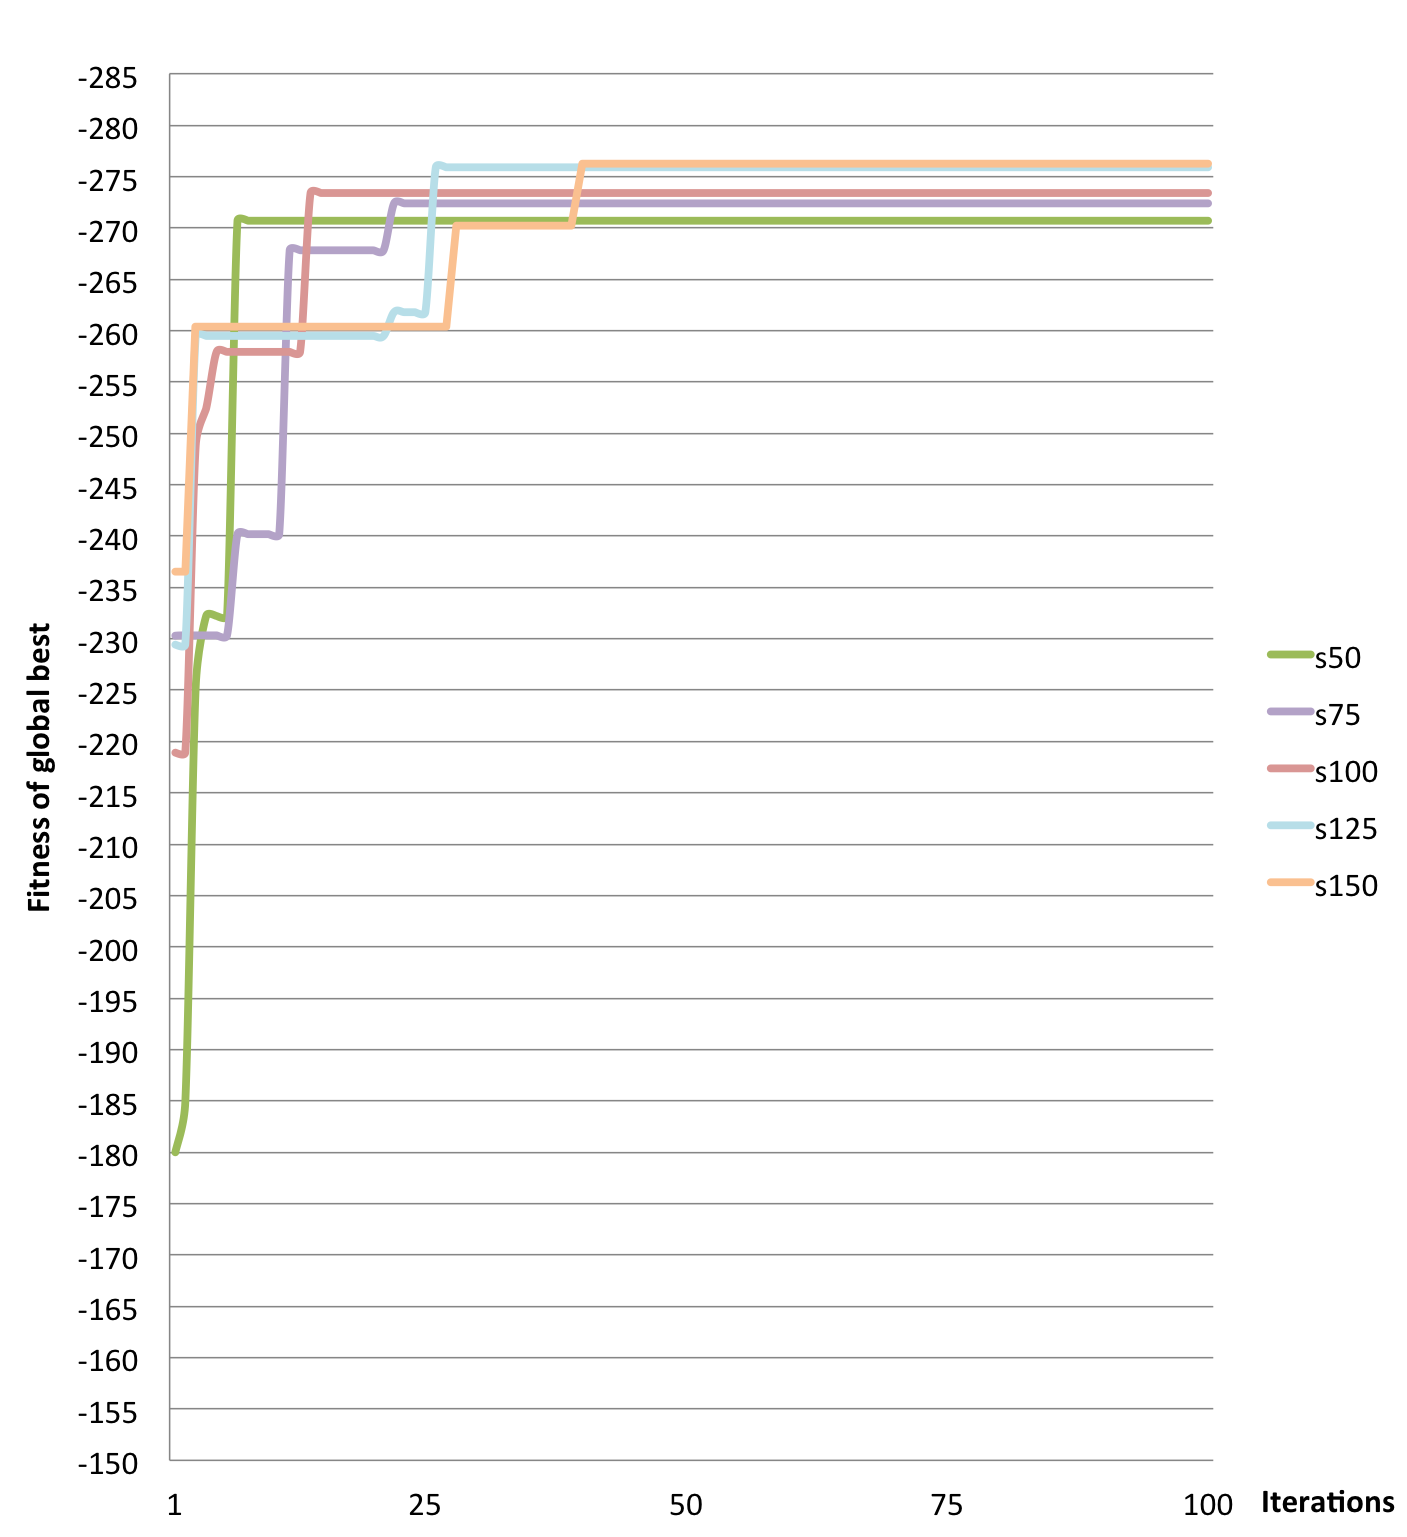
\includegraphics[width=4in]{assets/svsitest.png}
%  \end{center}
%  \caption{Evolution of Global Best Total Fitness ($TOTFIT$)}
%  \label{fig:svsitesting} 
%\end{figure}

\begin{figure}[H]
\begin{center}
  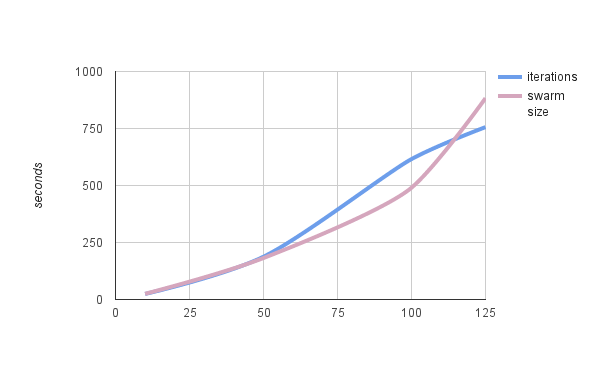
\includegraphics[width=5in]{assets/iterations_swarmsize_runtime.png}
  \end{center}
  \caption{Comparing runtime of increasing swarm size and number of iterations}
  \label{fig:svsiruntime} 
\end{figure}


Observing $s$ in Table \vref{table:pm1} in Appendix \ref{appendixC}, values below 50 sometimes produced ant colonies were no ants satisfied the initial Constraint \ref{itm:criteriaConnectedGraph} described in Section \vref{sec:algoConstraints}. When $s$ is 10, this occurs on average 16\% of the iterations and when the swarm size is 25 i occurs on average 0.5\% of the iterations. If no ant satisfy the initial constraint, no ant is either evaluated, and their results will be invalid.

Observing the produced results of parameter $E$ in Table \vref{table:pm1}, evaporating 50\% of the pheromone each iteration gave the best average total fitness and the second best average travel time. Evaporating 75\% gave the best average travel time, and the second best total fitness, but according to the formula described in Section \vref{subsec:parameterSettings_setup} 50\% is selected. As one can observe, the best produced results is achieved by a candidate value greater or equal to 50\%. The algorithm seems to benefit from the fact that a great amount of pheromone evaporates each iteration. We believe this is because it compensates for some of the randomness the parameter $CA$ produces, by quickly removing pheromone from edges that were once used, but later discarded. One can also observe that the worst results were achieved when $E$ was sat to 99\%. Even though the algorithm benefits from a large percentage of evaporated pheromones, it reaches a threshold were the percentage becomes too big. By removing 99\% of the pheromone an edge that is usually used a lot, but for some reason not used as much the given iteration, it is ``punished'' too hard. 
\newline

The amount of $AF$ determines the amount of Following Ants ($FA$) in the next iteration, and the $FA$ follow the same path as the best ants' paths unconditionally. Observing the results obtained in Table \vref{table:pm2}, the $TOTFIT$ value deteriorates when the amount of $AF$ becomes greater than 25\%. When the amount of $FA$ becomes too great, a relatively large number of normal ants will not be able to explore new (possibly better) routes in the next iterations, and the algorithm may suffer from a local optima. But as one also can see, 25\% computes better results than the candidate values below. Rewarding some good route sets seems to boost the algorithms performance to some degree, and 25\% is selected as the final parameter for $AF$.

Based on the produced results, the selected value of parameter $p_b$ is 0.9. The value of $p_b$ is strongly dependent on the value of $AF$, because the more following ants, the more pheromone added to each edge in the best route sets. To ensure that rewarding more edges with the selected amount of pheromone did not negatively affect the algorithm's performance when $AF$ is 25\%, the value of $p_b$ was tested with the new selected value of $AF$. As one can observe in Table \vref{table:pb_testing}, both $TOTFIT$ values have increased with the new increased value of $AF$, and the selected value for $p_b$ does not compute worse than when the $AF$ value was 10\%. The $ATT$ value decreases after the new value of $p_b$, and the value of $p_b$ will be the same as it initial was selected. 

The value of $CA$ is sat to 5\% based on the results shown in Table \vref{table:pm2}, meaning there is a 5\% probability that an ant is declared ``crazy'' and thus makes completely random decisions. The results in Table \vref{table:pm2} shows that the algorithm benefits from the fact that some ants are declared crazy. However, if the probability is greater than 25\%, both the average $ATT$ and the average $TOTFIT$ results worsen. Not surprisingly, is this because half or more of the colony acts completely random, and the algorithm looses some of the performing boosting features from ACO, such as favoring edges frequently walked by other ants. Like for $s$ below 50, a value of $CA$ above 50\% sometimes produces ant colonies were no ants satisfy the initial Constraint \ref{itm:criteriaConnectedGraph} described in Section \vref{sec:algoConstraints}. When such a large part of the colony acts randomly, several (and sometimes all) of these ants will create route sets that do not include every node in the network. The probability of creating a route set that does not contain all nodes are decreased in ``normal'' ants by the fact that they favor nodes they have not yet visited in the given route set.


The value of $CA$ is sat to 5\% based on the results shown in Table \vref{table:pm2} in Appendix \ref{appendixC}. The reader recalls from Section \vref{sec:algoInitialization} that this means that there is a 5\% probability that an ant is declared ``crazy'' and thus makes completely random decisions. The results in Table \vref{table:pm2} shows that the algorithm benefits from the fact that some ants are declared crazy, but also that if the probability is greater than 25\%, both the average $ATT$ and the average $TOTFIT$ results become worse. This is not very surprising, because if half of the colony or more acts randomly, the algorithm looses some of the performing boosting features from ACO, such as favoring edges frequently walked by other ants. Like for $s$ below 50, a value of $CA$ above 50\% sometimes produces ant colonies were no ants satisfy the initial Constraint \ref{itm:criteriaConnectedGraph} described in Section \vref{sec:algoConstraints}. This is again not very surprising, because when such a large part of the colony acts randomly, several (and sometimes all) of these ants will create route sets that do not include every node in the network. The probability of creating a route set that does not contain all nodes are decreased in ``normal'' ants by the fact that they favor nodes they have not yet visited in the given route set. 

\subsection{Experimental results}
\label{subsec:performanceComparison_results}

%---------------------- ACO VS SSO ---------------------

Table \vref{table:performanceComparison_ACOSSOBEST} presents the average produced results the proposed system (CSS) and the plain ACO implementation has produced. Representation of the best route set, having for routes, produced by CSS is seen in Fig. \vref{fig:bestRouteSet4}. Best, worst, average, and median produced results in addition to the standard deviation can be found in Appendix \ref{appendixC}, Table \vref{table:performanceComparison_ACOFull}.

    \begin{table}[H]
    \centering
    \begin{tabular}{|l||l|l|l|l|l|}
    \hline
    \textbf{System} & \textbf{$d_0(\%)$} & \textbf{$d_1(\%)$} & \textbf{$d_2(\%)$} & \textbf{$d_{unsat}(\%)$} & \textbf{$ATT$} \\
    \hline
    ACO avg & 81.92 & 16.13 & 1.86 & 0.09 & 10.43\\
    \hline
    CSS avg & 85.21 & 13.49 & 1.30 & 0.00 & 10.27\\
    \hline
    \end{tabular}
    \caption {The best route set, having four routes, constructed by the generic ACO implementation and the proposed system.}
    % 50 runs
    \label{table:performanceComparison_ACOSSOBEST}
    \end{table}

   

%-------------------- 4 route sets ---------------------
\begin{figure}[H]
    \begin{center}
    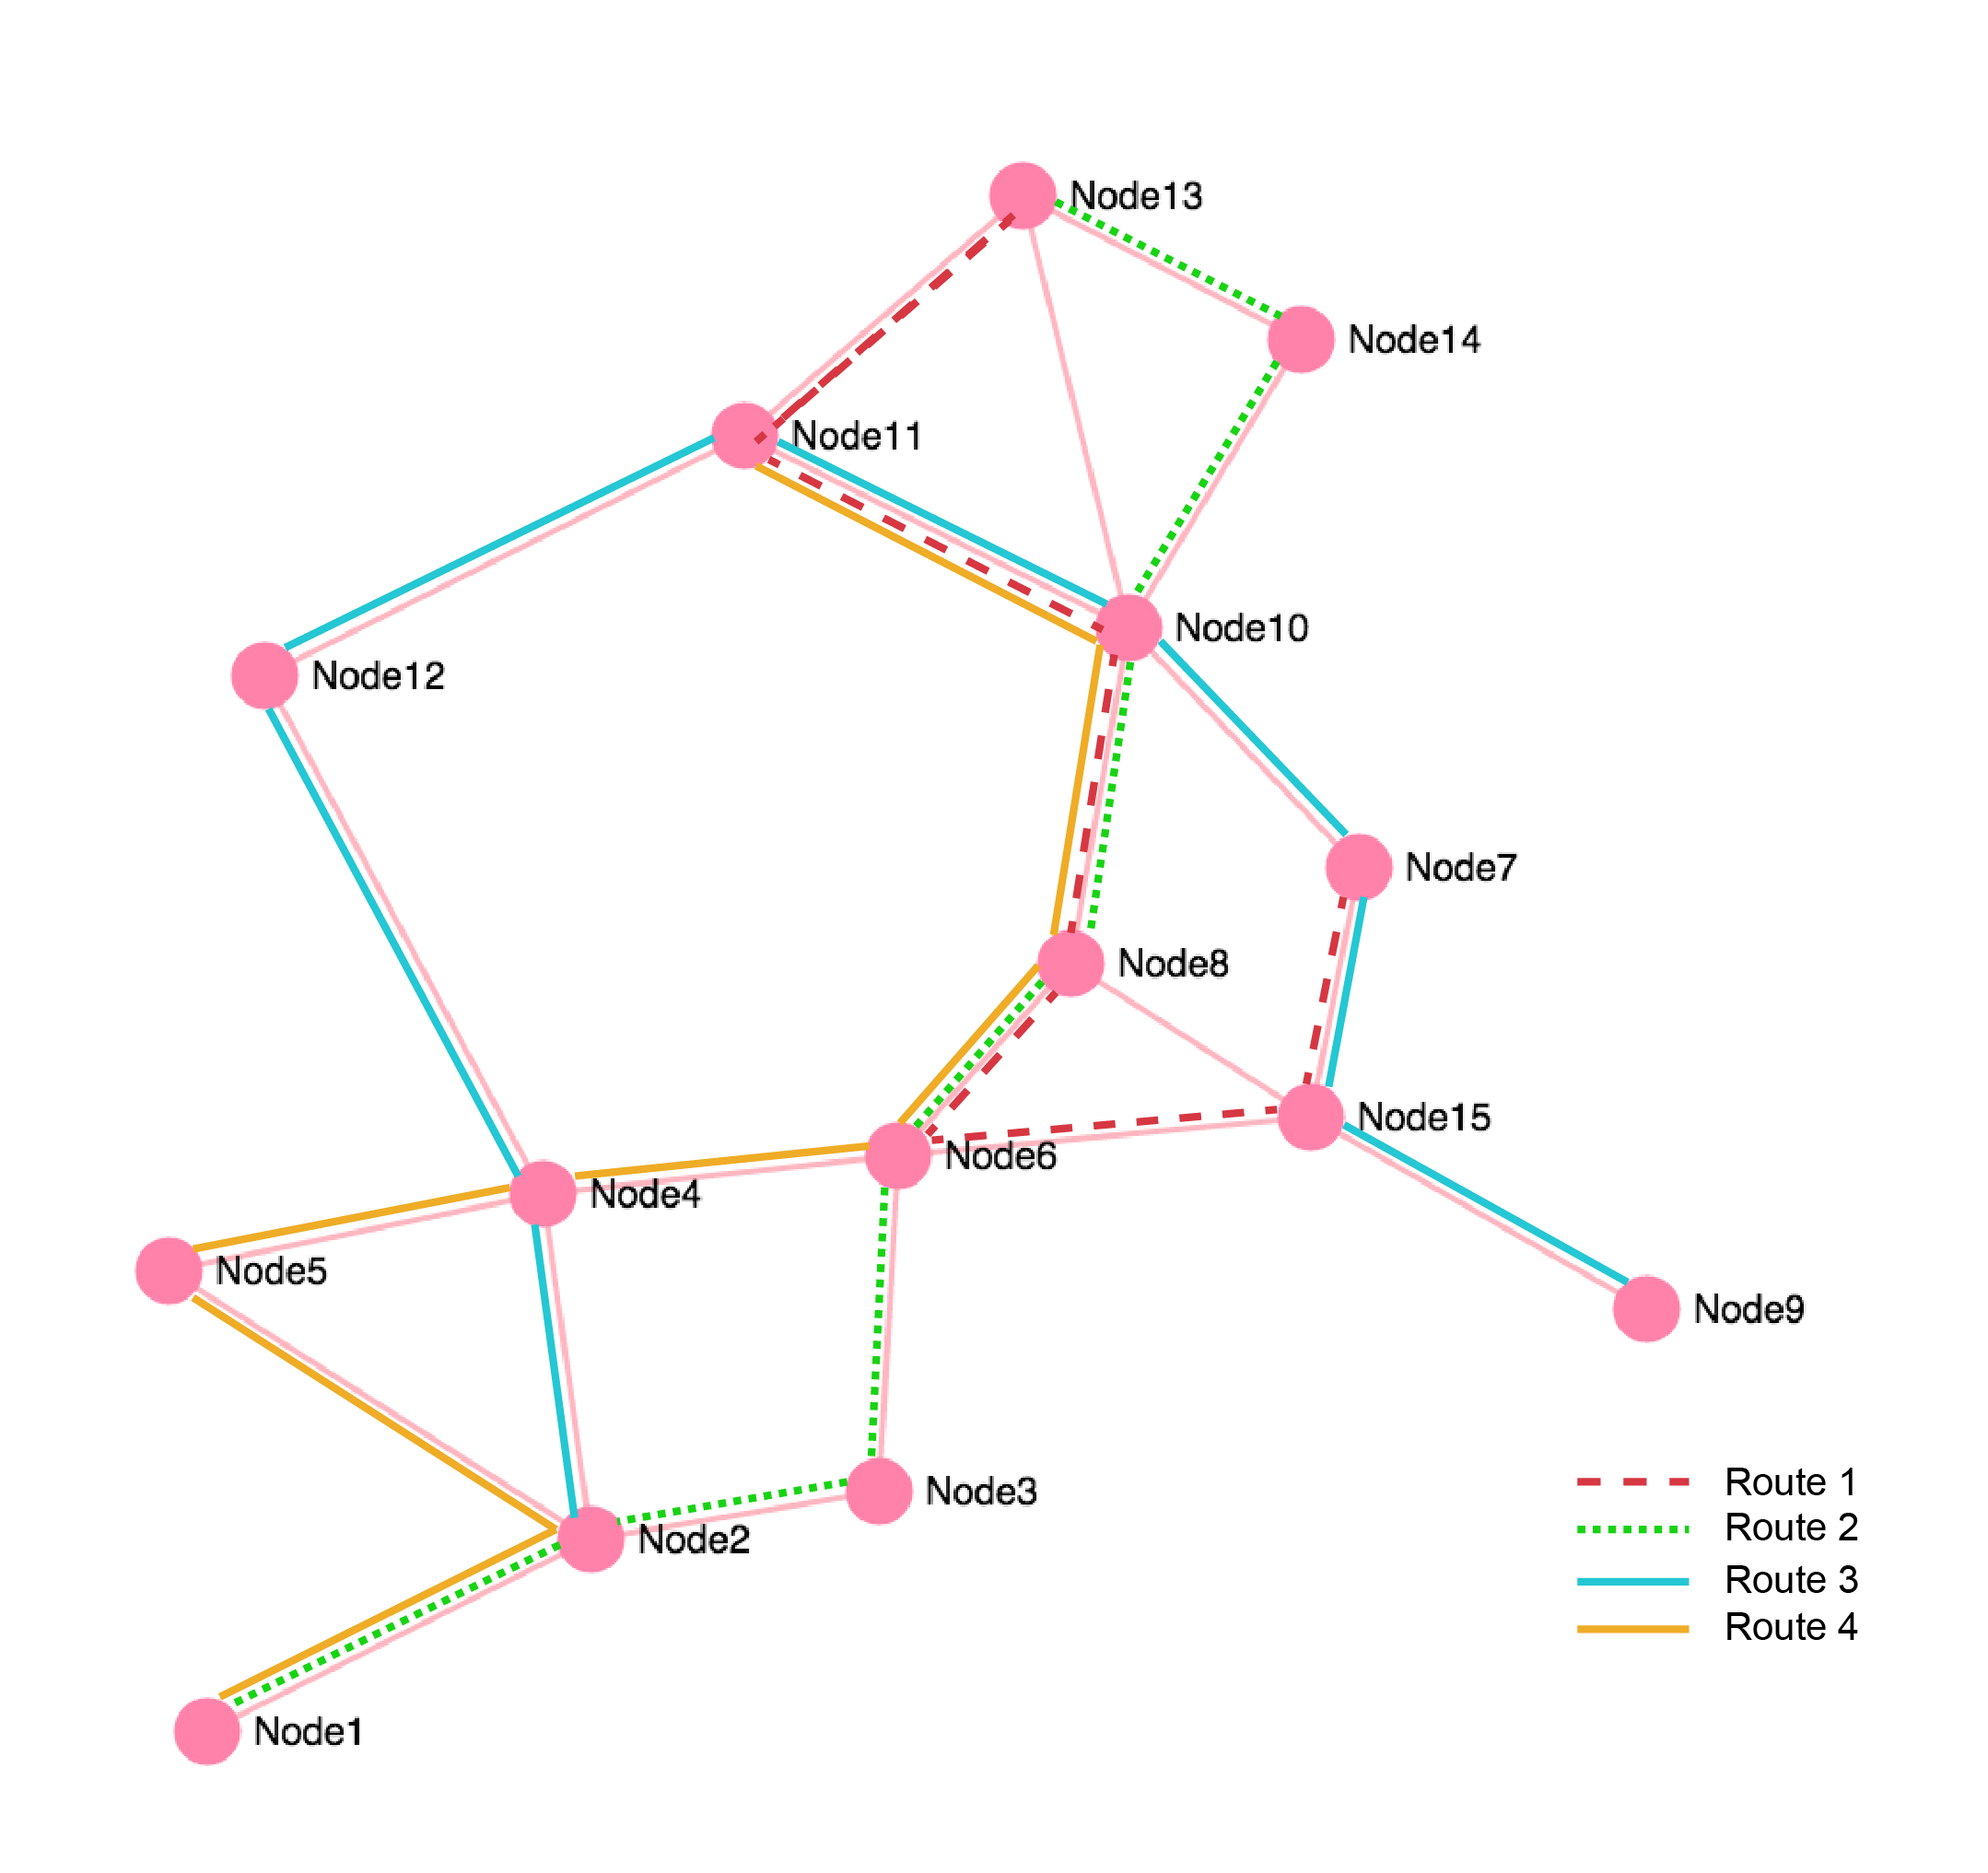
\includegraphics[width=4in]{assets/mandlnetwork_4routes.png}
    \end{center}
    \caption{Illustration of the best route set, having four routes, constructed by the proposed system on Mandl's Network}
    \label{fig:bestRouteSet4} 
\end{figure}

Table \vref{table:performanceComparison_4} presents the results produced by the proposed system, having four routes, and results from route sets constructed by other approaches. The table is sorted in ascending order with respect to the $ATT$ value.

\begin{table}[H]
	\centering
    \hspace*{-1.0cm}
    \begin{tabular}{|l||l|l|l|l|l|}
 	\hline
 	\textbf{System} & $d_0(\%)$ & $d_1(\%)$ & $d_2(\%)$ & $d_{unsat}(\%)$ & $ATT$ \\
 	\hline
    \citet{nikolic14} avg & 95.05 & 4.95 & 0.00 & 0.00 & -$^1$ \\
    \citet{kechagiopoulos14} best & 91.84 & 7.64 & 0.51 & 0.00 & 10.64 \\
    \citet{zhang10} & 91.46 & 8.54 & 0.00 & 0.00 & 10.65 \\
    \citet{kechagiopoulos14} avg & 90.52 & 8.75 & 0.73 & 0.00 & 10.71 \\
    \citet{chew12} best & 93.71 & 6.29 & 0.00 & 0.00 & 10.82 \\
    \citet{chew12} avg & 92.88 & 6.91 & 0.20 & 0.00 & 11.16 \\
    \citet{fan10} best & 93.26 & 6.74 & 0.00 & 0.00 & 11.37 \\
    \citet{fan10} SA$^2$ avg & 92.48 & 7.52 & 0.00 & 0.00 & 11.55 \\
    \citet{fan10} HC$^3$ avg & 91.83 & 8.17 & 0.00 & 0.00 & 11.69 \\
    \citet{chakroborty02} & 86.86 & 12.00 & 1.14 & 0.00 & 11.90 \\
    \citet{kidwai98} & 72.95 & 26.91 & 0.13 & 0.00 & 12.72 \\
    \citet{mandl79} & 69.94 & 29.93 & 0.13 & 0.00 & 12.90 \\
    \hline
    CSS Best & 87.73 & 10.98 & 1.28 & 0.00 & 10.03\\
    CSS Average & 85.21 & 13.49 & 1.30 & 0.00 & 10.27\\
    CSS Median & 85.81 & 13.29 & 1.09 & 0.00 & 10.26\\
    CSS Worst & 76.56 & 22.16 & 1.28 & 0.00 & 10.01\\
    Standard Deviation & 2.66 & 2.70 & 0.84 & - & 0.18\\
    %SSO Confidence interval$^b$ & ~ & ~ & ~ & ~ & ~ \\
    \hline
    \end{tabular}
    \caption {Comparing the best route set, having four routes, produced by the proposed system, with route sets constructed by other approaches.}
    \begin{itemize}[noitemsep]
    %\item[$^a$:] mintues per user
    \item[$^1$:] ATT not supplied
    \item[$^2$:] Simulated Annealing based system
    \item[$^3$:] Hill Climbing based system
    %\item[$^b$:] Confidence Interval with a confidence level of 95\%
    \end{itemize}
    \label{table:performanceComparison_4}
\end{table}

%-------------------- 6 route sets ---------------------
Table \vref{table:performanceComparison_4} presents the results produced by the proposed system, having six routes, and results from route sets constructed by other approaches. The table is sorted in ascending order with respect to the $ATT$ value.

\begin{figure}[H]
    \begin{center}
    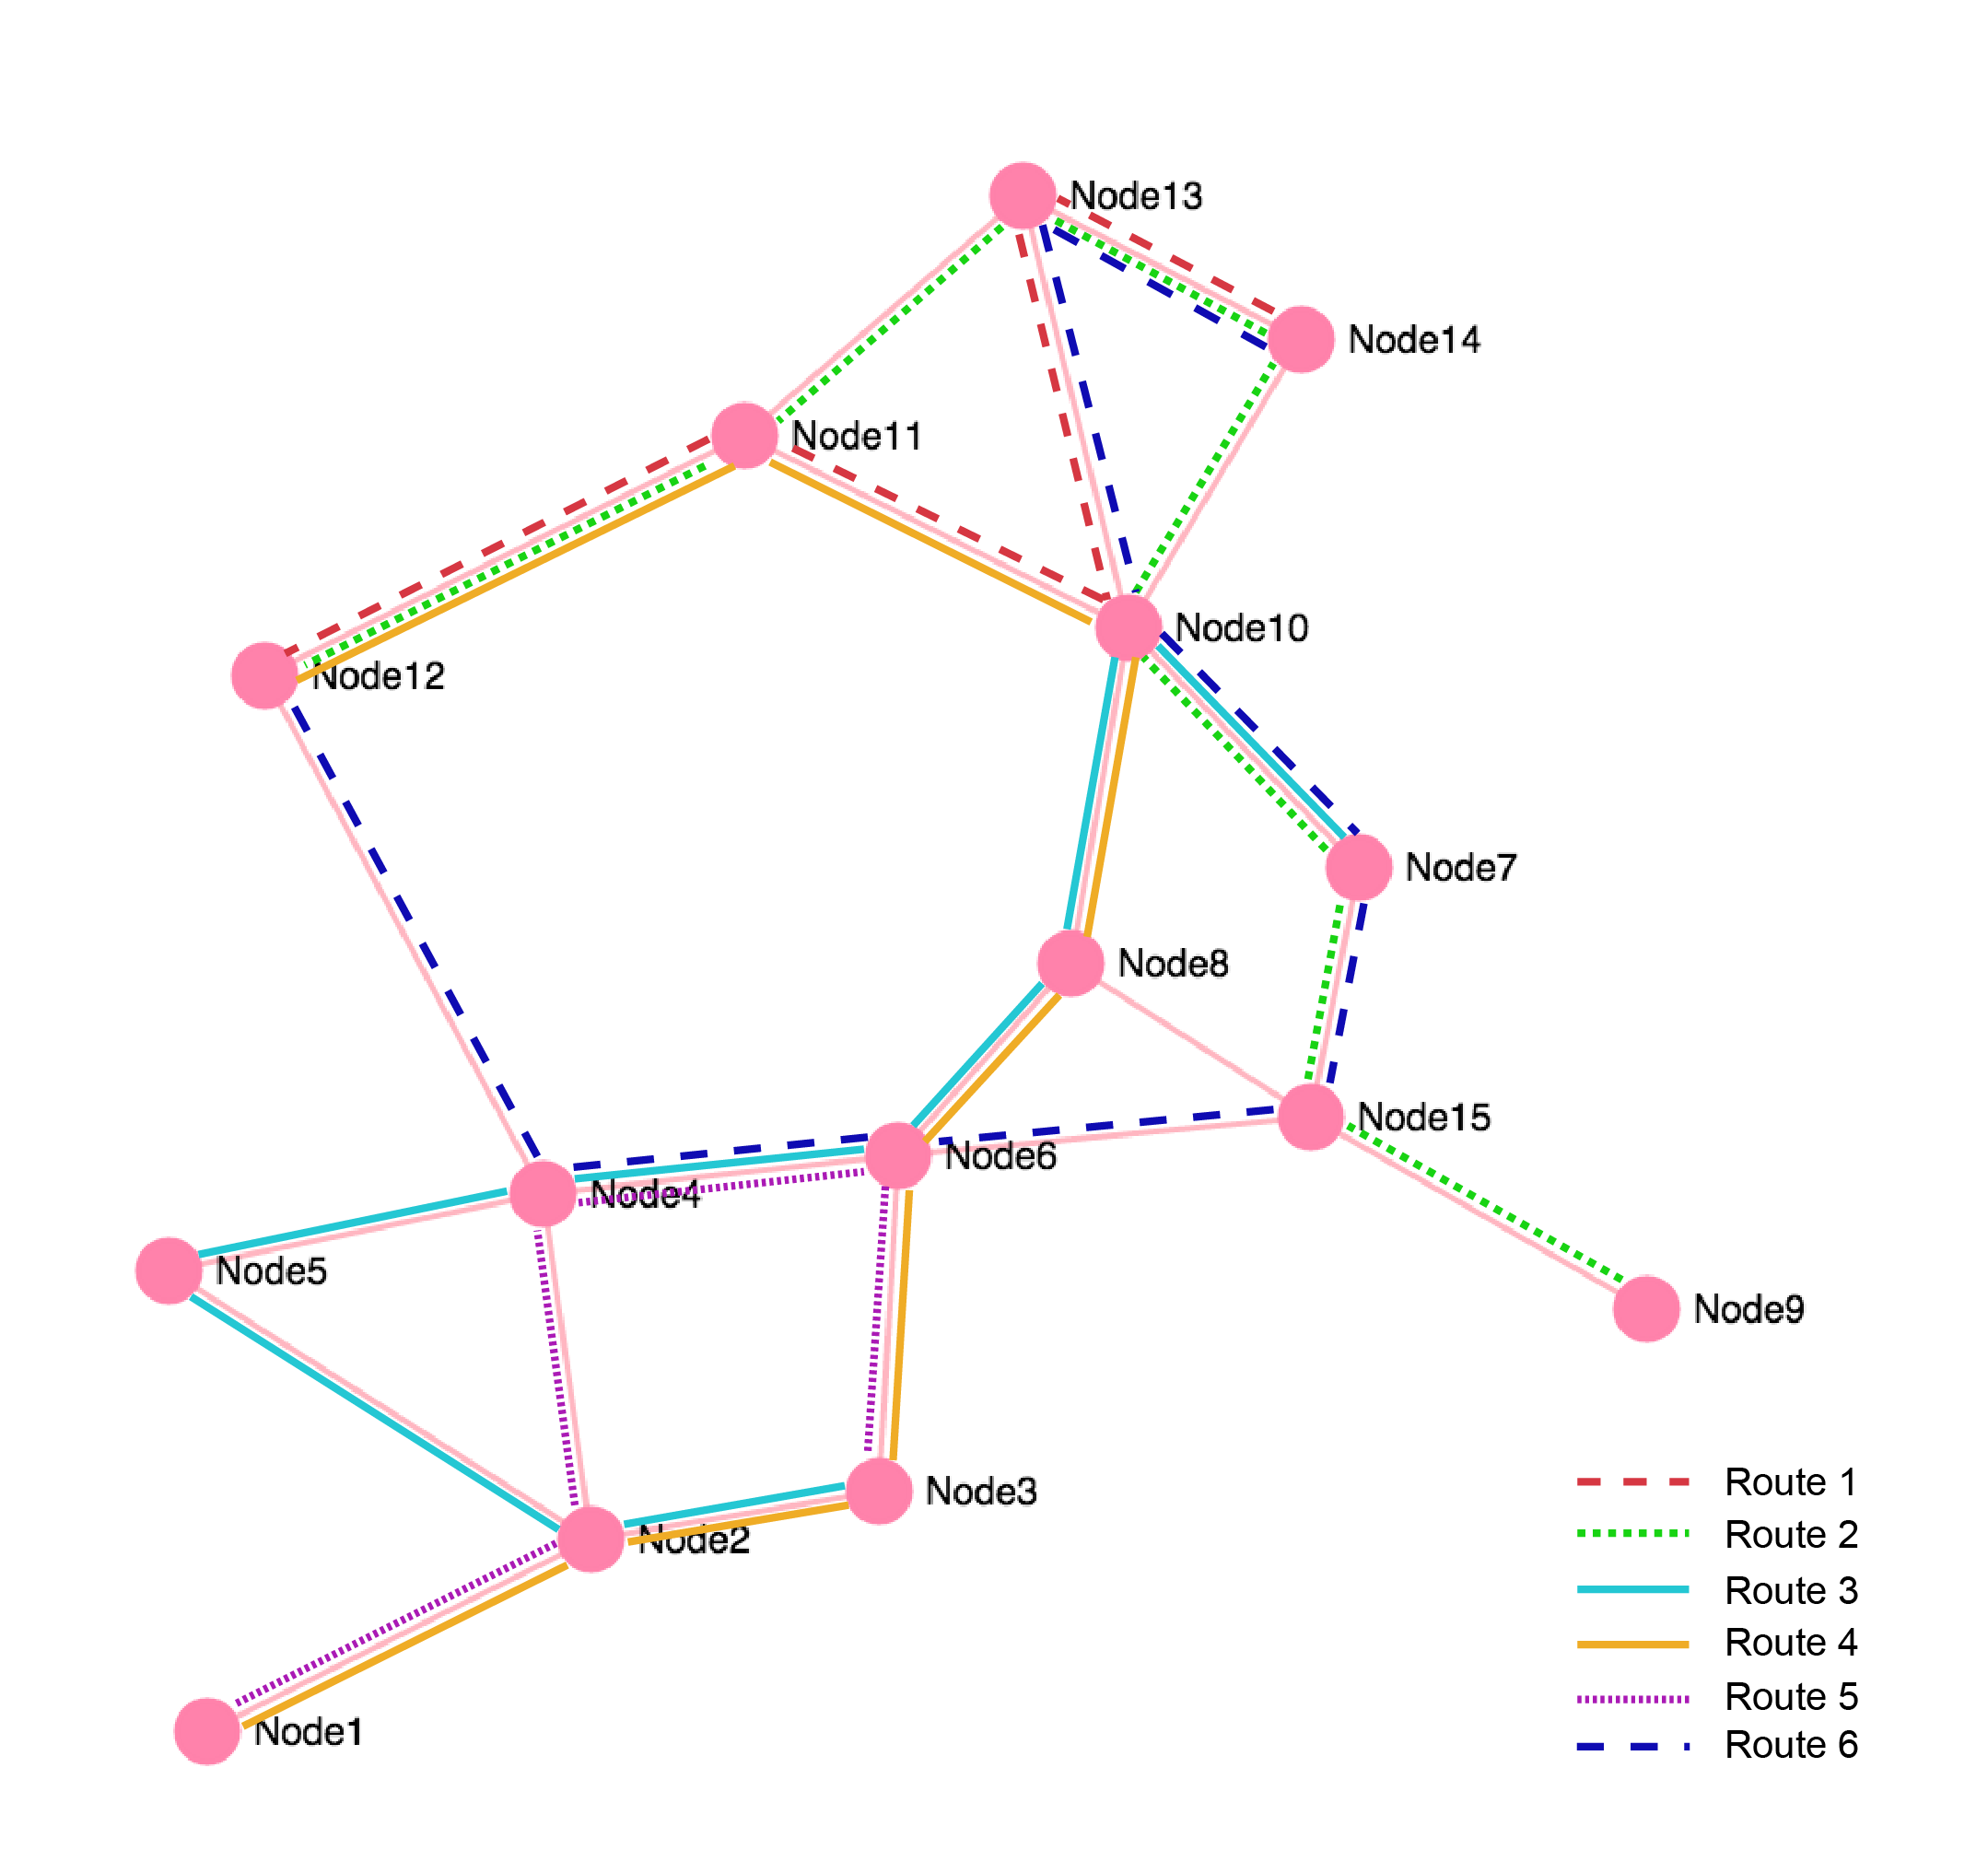
\includegraphics[width=4in]{assets/mandlnetwork_6routes.png}
    \end{center}
    \caption{Illustration of the best route set, having six routes, constructed by the proposed system on Mandl's Network}
    \label{fig:bestRouteSet6} 
\end{figure}

\begin{table}[H]
    \centering
    \hspace*{-1.0cm}
    \begin{tabular}{|l||l|l|l|l|l|}
    \hline
    \textbf{System} & $d_0(\%)$ & $d_1(\%)$ & $d_2(\%)$ & $d_{unsat}(\%)$ & $ATT$ \\
    \hline
    \citet{nikolic14} & 94.34 & 5.65 & 0.00 & 0.00 & - \\
    \citet{kechagiopoulos14} best & 96.21 & 3.47 & 0.32 & 0.00 & 10.23 \\
    \citet{kechagiopoulos14} avg & 95.62 & 4.28 & 0.10 & 0.00 & 10.28 \\
    \citet{chew12} best & 95.57 & 4.43 & 0.00 & 0.00 & 10.28 \\
    \citet{chakroborty02} & 86.04 & 13.96 & 0.00 & 0.00 & 10.30 \\
    \citet{fan10} best & 91.52 & 8.48 & 0.00 & 0.00 & 10.48  \\
    \citet{zhang10} & 91.12 & 8.88 & 0.00 & 0.00 & 10.50 \\
    \citet{chew12} avg & 93.85 & 5.88 & 0.24 & 0.03 & 10.51 \\
    \citet{fan10} SA avg & 90.87 & 8.74 & 0.39 & 0.00 & 10.65 \\
    \citet{fan10} HA avg & 90.23 & 9.26 & 0.51 & 0.00 & 11.69 \\
    \citet{kidwai98} & 77.92 & 19.62 & 2.40 & 0.00 & 10.78 \\
    \citet{baaj91} & 78.61 & 21.39 & 0.00 & 0.00 & 11.86 \\
    \hline
    CSS Best & 89.53 & 9.25 & 1.22 & 0.00 & 10.03\\
    CSS Average & 87.17 & 12.0 & 0.82 & 0.00 & 10.11\\
    CSS Median & 87.93 & 10.98 & 0.77 & 0.00 & 10.03\\
    CSS Worst & 82.47 & 17.41 & 0.13 & 0.00 & 10.03\\
    Standard Deviation & 2.74 & 2.78 & 0.63 & - & 0.14\\
    \hline
    \end{tabular}
    \caption {Comparing the best route set, having six routes, produced by the proposed system with route sets constructed by other approaches.}
    \label{table:performanceComparison_6}
\end{table}

%-------------------- 7 route sets ---------------------
Table \vref{table:performanceComparison_4} presents the results produced by the proposed system, having seven routes, and results from route sets constructed by other approaches. The table is sorted in ascending order with respect to the $ATT$ value.

\begin{figure}[H]
    \begin{center}
    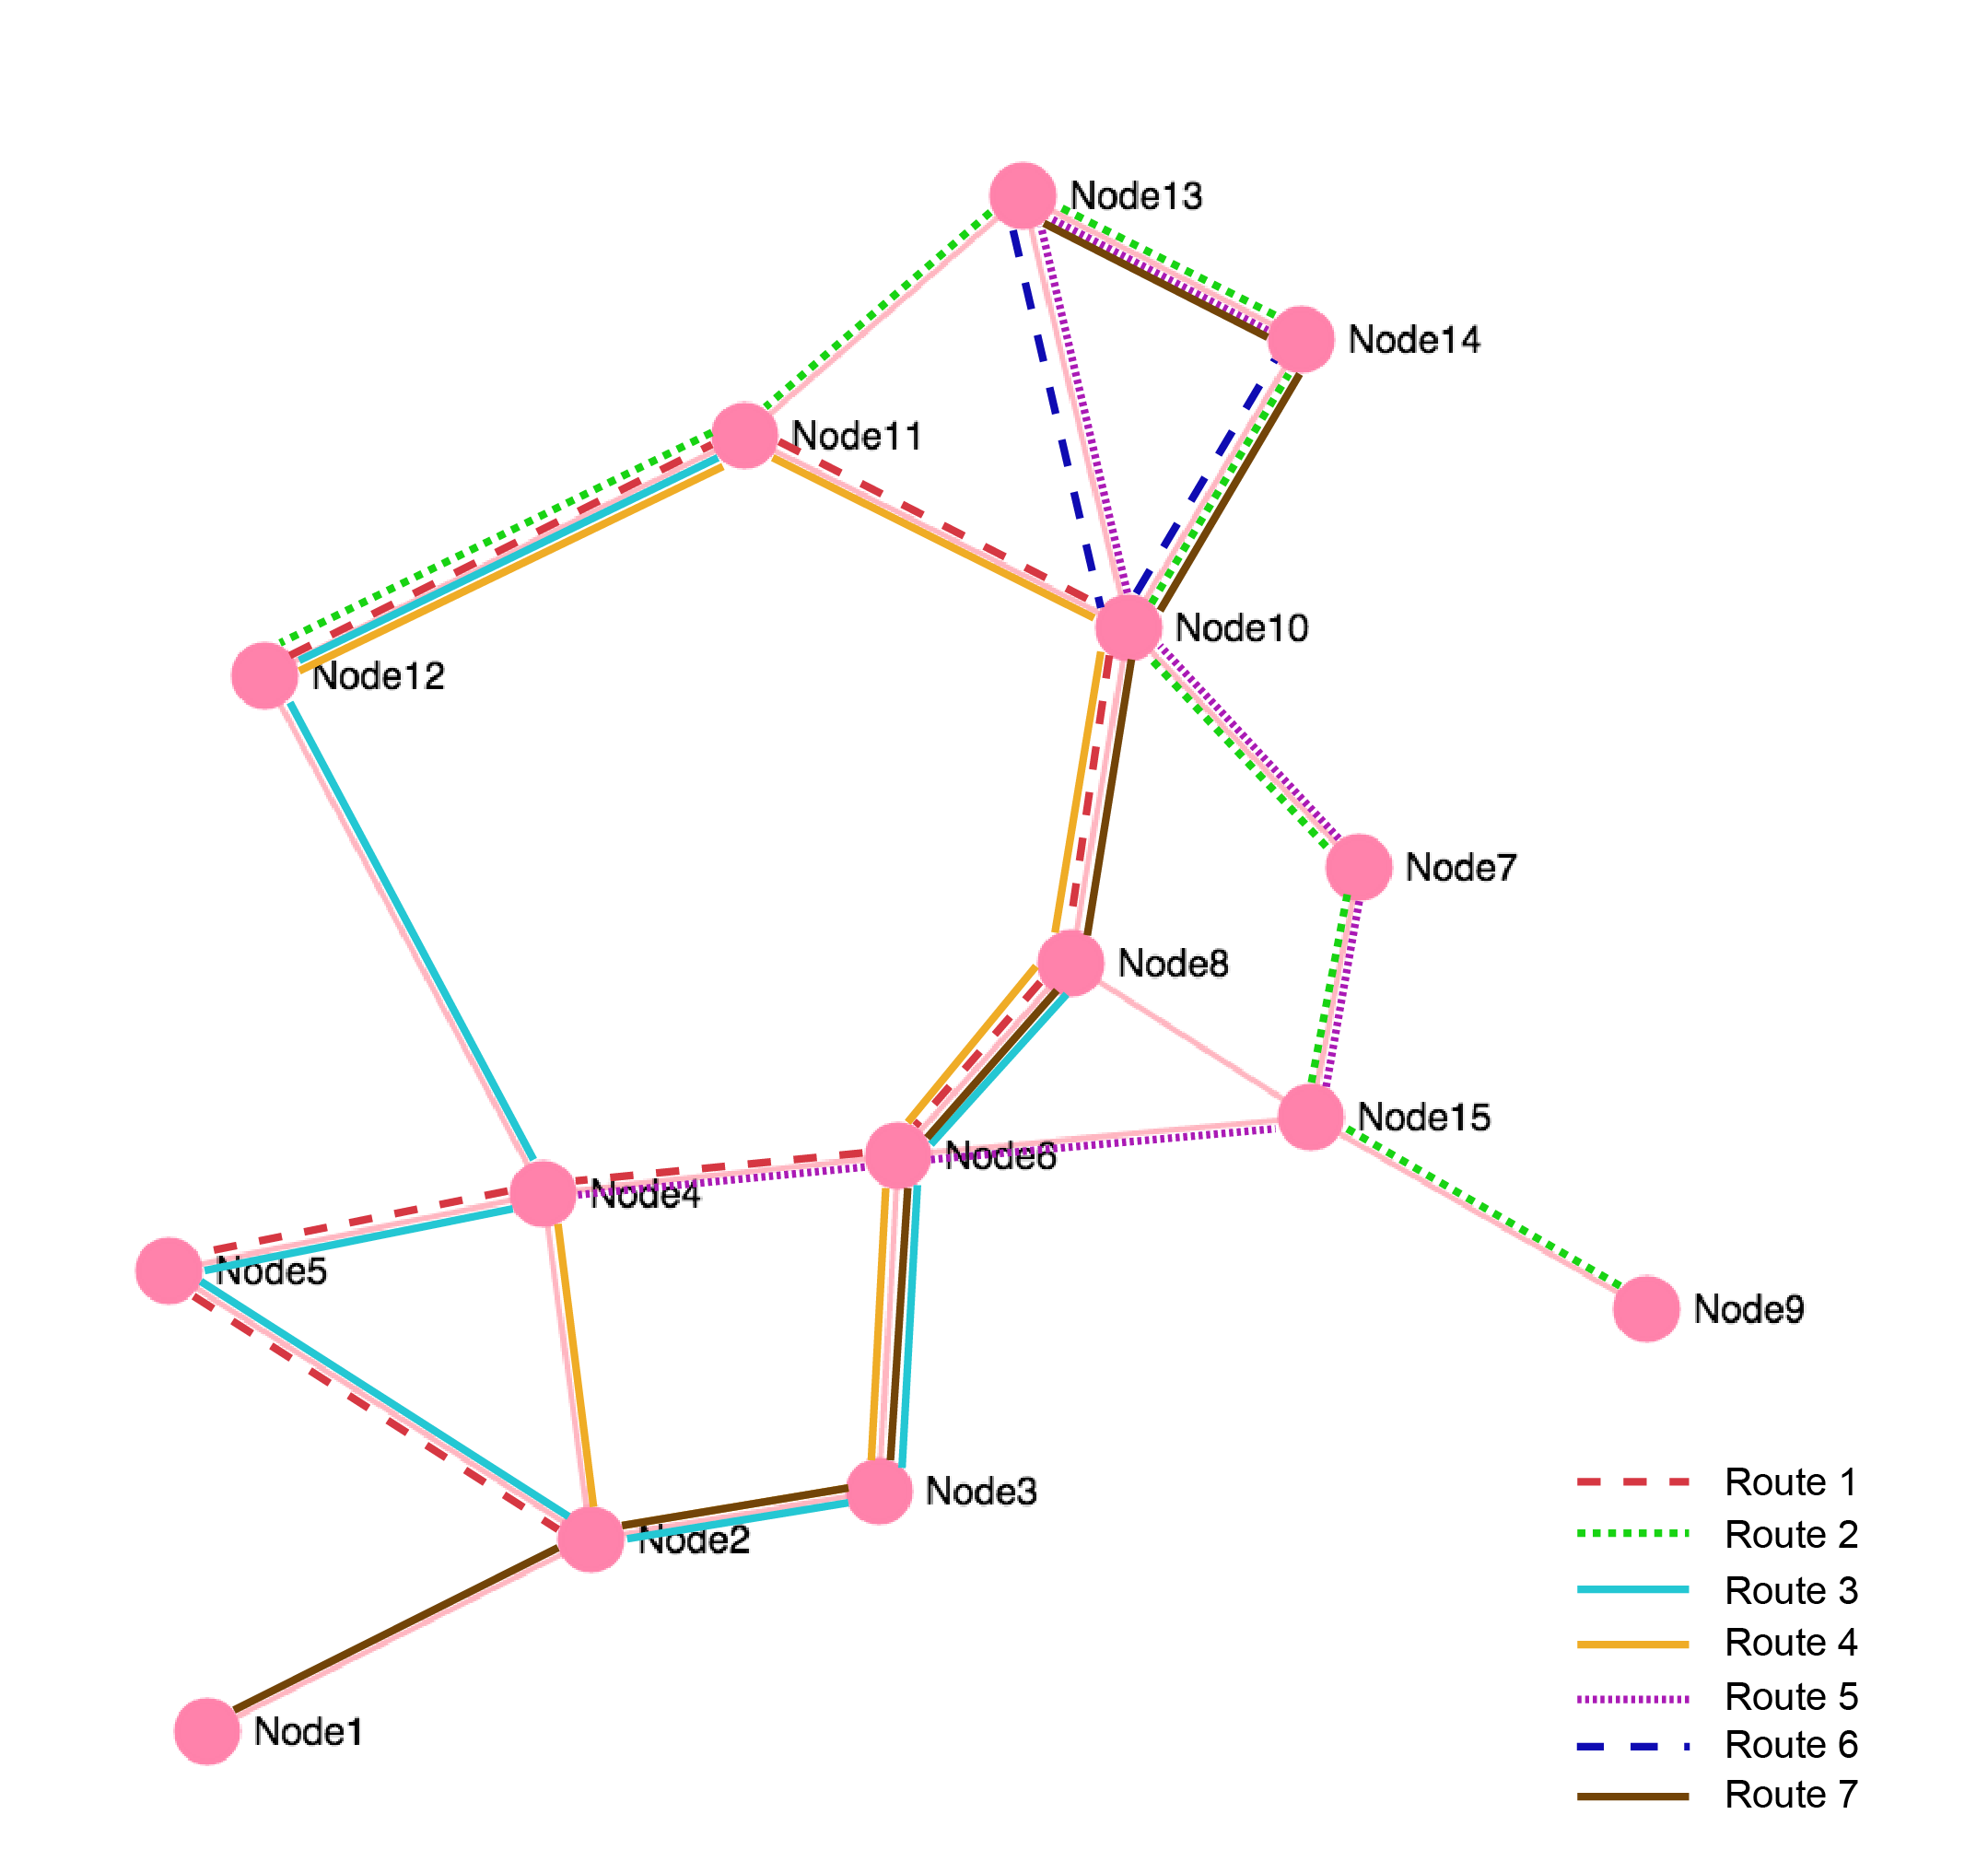
\includegraphics[width=4in]{assets/mandlnetwork_7routes.png}
    \end{center}
    \caption{Illustration of the best route set, having seven routes, constructed by the proposed system on Mandl's Network}
    \label{fig:bestRouteSet7} 
\end{figure}

\begin{table}[H]
    \centering
    \hspace*{-1.0cm}
    \begin{tabular}{|l||l|l|l|l|l|}
    \hline
    \textbf{System} & $d_0(\%)$ & $d_1(\%)$ & $d_2(\%)$ & $d_{unsat}(\%)$ & $ATT$ \\
    \hline
    \citet{nikolic14} & 94.41 & 5.59 & 0.00 & 0.00 & - \\
    \citet{chakroborty02} & 89.15 & 10.85 & 0.00 & 0.00 & 10.15 \\
    \citet{kechagiopoulos14} best & 97.17 & 2.83 & 0.00 & 0.00 & 10.16 \\
    \citet{kechagiopoulos14} avg & 96.55 & 3.45 & 0.01 & 0.00 & 10.23 \\
    \citet{chew12} best & 95.57 & 4.42 & 0.00 & 0.00 & 10.27 \\
    \citet{chew12} avg & 96.47 & 3.53 & 0.00 & 0.00 & 10.31 \\
    \citet{fan10} best & 93.32 & 7.13 & 0.32 & 0.00 & 10.42  \\
    \citet{zhang10} & 92.89 & 7.11 & 0.00 & 0.00 & 10.46 \\
    \citet{fan10} SA avg & 92.47 & 6.95 & 0.58 & 0.00 & 10.62 \\
    \citet{kidwai98} & 93.91 & 6.09 & 0.00 & 0.00 & 10.70 \\
    \citet{fan10} HC avg & 92.21 & 7.13 & 0.66 & 0.00 & 10.74 \\
    \citet{baaj91} & 80.99 & 19.01 & 0.00 & 0.00 & 12.50 \\
    \hline
    CSS Best & 89.85 & 8.67 & 1.48 & 0.00 & 10.03\\
    CSS Average & 88.49 & 10.72 & 0.79 & 0.00 & 10.08\\
    CSS Median & 88.12 & 10.92 & 0.90 & 0.00 & 10.03\\
    CSS Worst & 83.94 & 15.93 & 0.13 & 0.00 & 10.01\\
    Standard Deviation & 2.29 & 2.32 & 0.42 & - & 0.08\\
    \hline
    \end{tabular}
    \caption {Comparing the best route set, having seven routes, produced by the proposed system with route sets constructed by other approaches.}
    \label{table:performanceComparison_7}
\end{table}
%-------------------- 8 route sets ---------------------
Table \vref{table:performanceComparison_4} presents the results produced by the proposed system, having eight routes, and results from route sets constructed by other approaches. The table is sorted in ascending order with respect to the $ATT$ value.

\begin{figure}[H]
    \begin{center}
    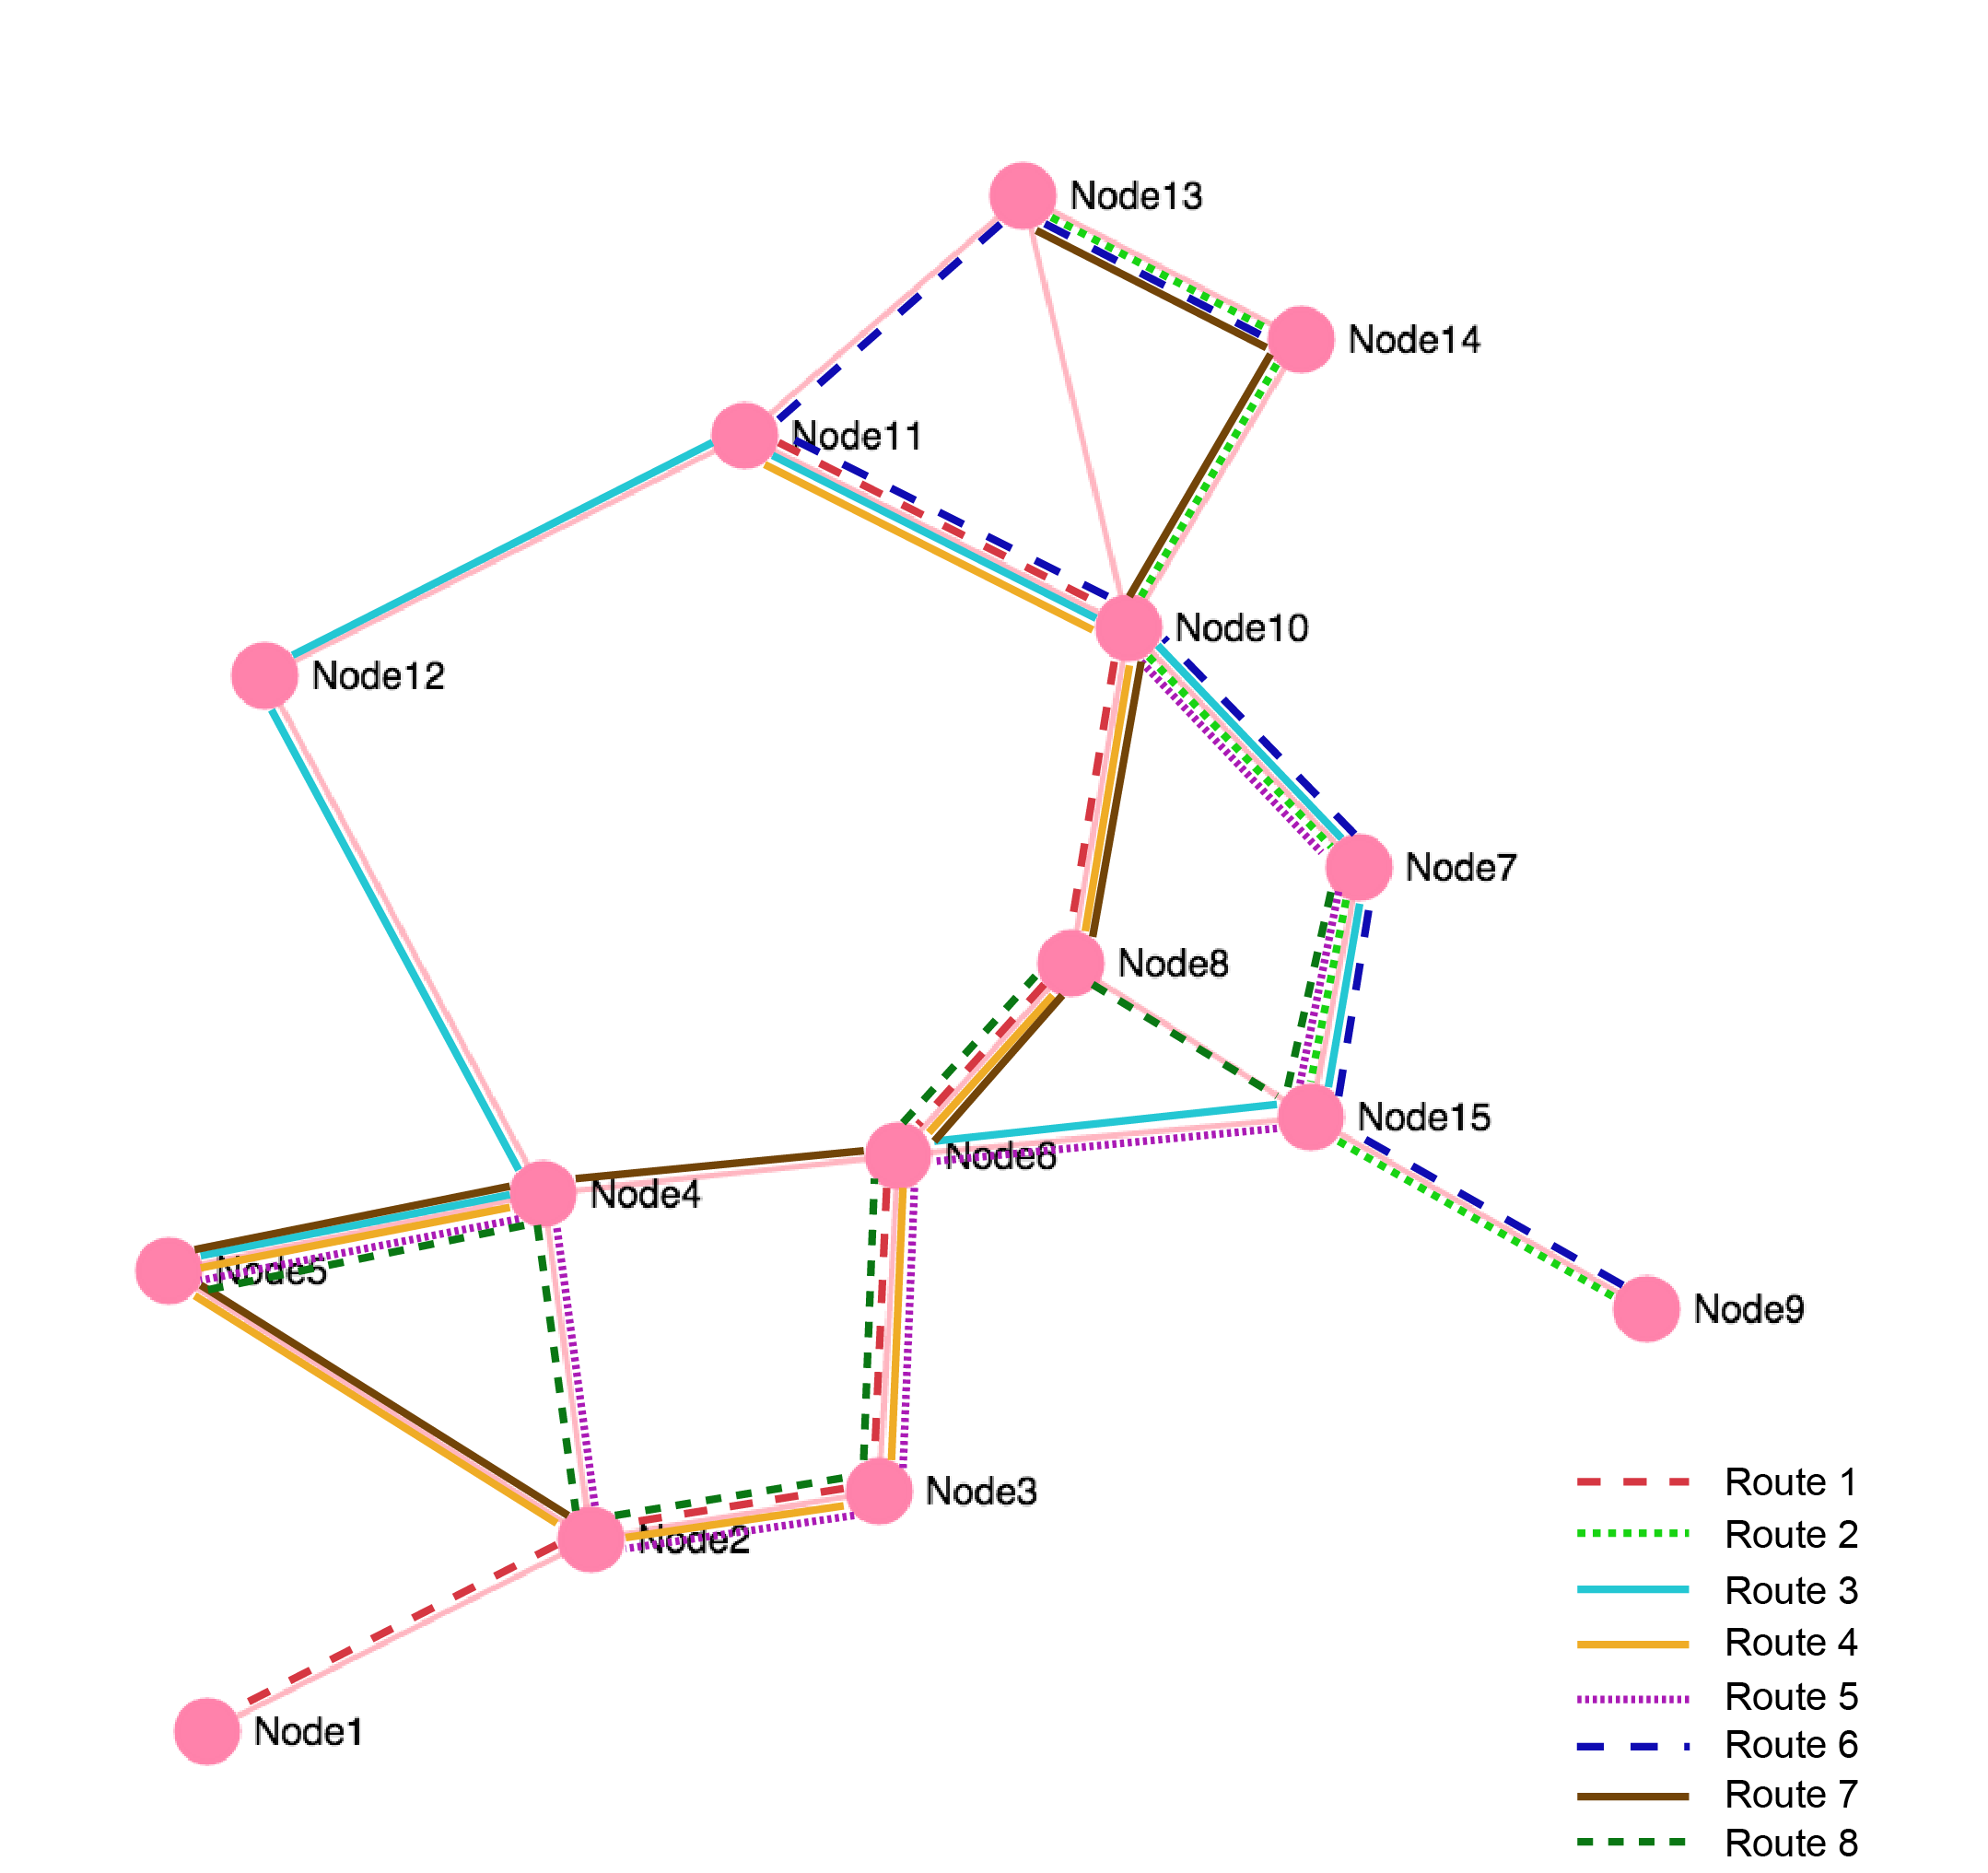
\includegraphics[width=4in]{assets/mandlnetwork_8routes.png}
    \end{center}
    \caption{Illustration of the best route set, having eight routes, constructed by the proposed system}
    \label{fig:bestRouteSet8} 
\end{figure}

    \begin{table}[H]
    \centering
    \hspace*{-1.0cm}
    \begin{tabular}{|l||l|l|l|l|l|}
    \hline
    \textbf{System} & $d_0(\%)$ & $d_1(\%)$ & $d_2(\%)$ & $d_{unsat}(\%)$ & $ATT$ \\
    \hline
    \citet{nikolic14} & 96.40 & 3.60 & 0.00 & 0.00 & - \\
    \citet{kechagiopoulos14} best & 97.75 & 2.25 & 0.00 & 0.00 & 10.13 \\
    \citet{kechagiopoulos14} avg & 97.47 & 2.53 & 0.00 & 0.00 & 10.17 \\
    \citet{chew12} best & 97.82 & 2.18 & 0.00 & 0.09 & 10.19 \\
    \citet{chew12} avg & 96.16 & 3.84 & 0.00 & 0.09 & 10.31 \\
    \citet{fan10} best & 94.54 & 5.46 & 0.00 & 0.00 & 10.36 \\
    \citet{zhang10} & 93.14 & 6.86 & 0.00 & 0.00 & 10.42 \\
    \citet{chakroborty02} & 90.38 & 9.58 & 0.00 & 0.00 & 10.46 \\
    \citet{fan10} Simulated Annealing & 93.65 & 5.88 & 0.47 & 0.00 & 10.58 \\
    \citet{fan10} Hill Climbing & 93.23 & 6.18 & 0.59 & 0.00 & 10.69 \\
    \citet{kidwai98} & 84.73 & 15.27 & 0.00 & 0.00 & 11.22 \\
    \citet{baaj91} & 79.96 & 20.04 & 0.00 & 0.00 & 11.86 \\ 
    \hline
    CSS Best & 91.01 & 7.9 & 1.09 & 0.00 & 10.01\\
    CSS Average & 89.16 & 10.05 & 0.8 & 0.00 & 10.06\\
    CSS Median & 88.7 & 10.21 & 0.77 & 0.00 & 10.03\\
    CSS Worst & 92.42 & 6.81 & 0.77 & 0.00 & 10.08\\
    Standard Deviation & 2.24 & 2.14 & 0.68 & - & 0.07\\
    \hline
    \end{tabular}
    \caption {Comparing the best route set, having eight routes, produced by the proposed system with route sets constructed by other approaches.}
    \label{table:performanceComparison_8}
    \end{table}

%---------------------- Execution time ---------------------



%Table \vref{table:performanceComparison_runtime} shows the average runtime for each run with 50 runs.


\subsection{Scalability Experiments}
\label{subsec:scalabilityExperiments_results}

\begin{table}[H]
    \centering
    \begin{tabular}{|l|l|l|l|l|l|}
        \hline
        Test case & Method & TOTFIT & ATT & Running time(sec) \\
        \hline
        1 & 1 & -61.42 & 17.54 & 6764 \\
        1 & 2 & -167.12 & 17.36 & 68018 \\
        
        \hline
    \end{tabular}
    \caption{Mumford0 execution time in seconds, method1 vs method2 \emph{\color{blue} gammel algorithme}}
    \label{table:results_mumford}
\end{table}

The reader recalls from Section \vref{sec:f1},  \textit{Method 1} is where the path with the shortest traveling time, not considering any transitions, is chosen. In the second method, \textit{Method 2}, the transitions is considered, and chooses the path with the shortest traveling time, including transfer penalties.


%-------Mumford3--------
%Exception in thread "main" org.neo4j.graphdb.TransactionFailureException: Could not create token

%Caused by: org.neo4j.kernel.impl.store.UnderlyingStorageException: Id capacity exceeded: 65536 is not within bounds
 %[0; 65535] for Neo4jTest1/neostore.relationshiptypestore.db.id


\begin{table}[H]
    \centering
    \hspace*{-1.0cm}
    \begin{tabular}{|l|l|l|l|l|l|l|l|l|}
        \hline
        Test case & Nodes & Edges & Min/max nodes  & $d_0$ & $d_1$ & $d_2$ & $d_{unsat}$ & $ATT$\\
        \hline
        Mumford0 & 30 & 90 & 2/15 & & & & &\\
        Mumford1 & 70 & 210 & 10/30 & & & & &\\
        Mumford2 & 110 & 385 & 10/22 & & & & &\\
        Mumford3$^a$ & 127 & 425 & 12/25 & & & & &\\
        \hline
    \end{tabular}
    \caption{Data set Mumford}
    \begin{itemize}[noitemsep]
    \item[$^a$:] Could not create token - Id capacity exceeded: 65536 is not within bounds
    \end{itemize}
    \label{table:dataSet_mumford}
\end{table}
It is worth mentioning, that the amount of iterations and swarm size is sat to 50, and the number of runs is 10. \emph{\color{blue} TODO.}

\chapter{Evaluation and Conclusion}
\label{evaluationAndConclusion}
\section{Evaluation}

When evaluating your results, avoid drawing grand conclusions, beyond that which your results can in fact support. Further, although you may have designed your experiments to answer certain questions, the results may raise other questions in the eyes of the reader. It is important that you study the graphs/tables to look for unusual features/entries and discuss these as well as discussing the main findings in the results. 

\subsection{Parameter Settings}
Remember:
\begin{itemize}
\item $p_v$, $p_b$: giving these values a higher number, results in awarding the local best ants edges by giving them more pheromone, which we observed gave worse results, \emph{\color{red}because get stuck at local optima? blabla}
\item with 100\% crazy ants, the ants did not manage to find a solution \emph{\color{red}because...}. 
\item 0\% crazy ants gave worse results than both 5\% and 10\% CA, where we can conclude that some crazy ants is better than none. But, as we see in the results, more than 10\% CA gives worse results than 0\% CA, so we can conclude that it does not mean the more crazy ants, the better results regarding the final results. But some CA is good for the colony:)
\item Our start values - 10\% on $p_e$, $BR$, $FA$, and $CA$, was actually the best values all along. We could have set these to have worse values in the beginning of the test experiment, and receiving increasing results concerning $TOTFIT$ and $ATT$, but \emph{\color{red} we set the start values to be what we though was best, because???, and with this conclude that our instinct regarding these values was the best.}
\item 100\% and 50\% FA was better than having 0\% following ants; can we conclude that it is better to have following ants, than not have following ants ?
\item Ant colony size ,$s$, parameter testing will be optimized for Mandl network only.
\end{itemize}

\subsection{Neo4j}

Whether Neo4J is suited. Advantages / disadvantages of using a graph database in our implementation (research question 3a)
\subsection{Evaluation Criteria}
%Denne er kopiert men skal skrives om:
%This section is dedicated to the issue of evaluating the implementation and this project as a whole. Evaluation is an issue much discussed in the field of artificial intelligence(AI). Cohen and Howe claims many papers do an inadequate job of evaluating the result of their AI systems. The systems described in question in this thesis have an inherent black-box nature. This means it is inconceivable to understand the rationale behind why the system delivers its result. his complicates the evaluation. An evaluation with clear relative benchmarks is thus important and to avoid any pitfalls that invalidate the results. Examples of this are overfitting or data leakage. In this effort Cohen and Howe’s five stage process is used for evaluating empirical AI systems.
(Evaluating the implementation and this project as a whole.)
As initiated in Section\vref{sec:structuredLiteratureReview}, \citet{cohen88} introduced a five-stage model for evaluating research in terms of a five-stage cycle. This development process should be run as iterative cycles, and is begun answered in \vref{sec:structuredLiteratureReview} and \vref{sec:problemStatement}.
\begin{enumerate}
\item a topic is refined to a task and a view of how to accomplish the task
\item the view is refined to a specific method
\item a program is developed to implement the method
\item experiments are designed to test the program
\item the experiments are run
\end{enumerate} 
\subsection{Evaluating Methods}
%1. How is the method an improvement over existing technologies?
%(a) Does it account for more situations? (input)
%(b) Does it produce a wider variety of desired behaviors? (output)
%(c) It the method expected to be more efficient? (space, solution time, development time, etc.)
%(d) Does it hold more promise for further development? (for example, due to the opening of a new paradigm)

%2. Is there a recognized metric for evaluating the performance of your method? (eg. normative, cognitively valid, etc.)
As mentioned, Mandl's benchmark problem is used by several researchers and the metric for evaluating is established. A good solution is one that provides a low average travel time, a high percentage of passengers traveling directly or with one transfer form the origin to their destination and a low percentage of both passengers transferring twice and \texit{unsatisfied} passengers. The reader recalls from Section \vref{sec:algoEvaluation} that an unsatisfied passenger is one that needs to transfer more than two times. Not only are these metric used by other researchers, and therefore makes it easy to compare our results, but they also corresponds to our goal described on page \pageref{itm:goal} of increasing  the number of public transportation passengers. 

%3. Does it rely on other methods? (Does it require input in a particular form or preprocessed? Does it require to a certain type of knowledge base or routines?)
The proposed method requires input on a particular form. Both nodes and their coordinates, travel time between nodes and the demand between nodes needs to be provided on a particular form in an .txt-document. This may be considered as a weakness of the method, but implementing support for retrieving the mentioned data on another form are considered as fairly easy. 

%4. What are the underlying assumptions? (know limitations, scope of expected input, scope of desired output, expected performance criteria, etc.)
An assumption made by the authors is that a route represent possibilities for traveling in both directions. 

%5. What is the scope of the method?
%(a) How extendible is it? Will it scale up to a large knowledge base?
\emph{\color{blue} TODO: ``How extendible is it? Will it scale up to a large knowledge base?''. Dette må skrives om når Mumford testene er ferdig}
%(b) Does it address exactly the task? portions of the task? a class of tasks?
%(c) Could it, or parts of it, be applied to other problems? Is it specially tuned for a particular example?
The parameters tested and used are specifically tuned for Mandl's Transit Network containing 4 routes, with maximum 8 nodes i one route. This may be considered a weakness because the parameters could possibly have different ideal values for other problems. 


%(d) Does it transfer to more complicated problems? (perhaps more knowledge intensive or more/less constrained or with more complex interactions)
\emph{\color{blue} TODO: ``Does it transfer to more complicated problems?''. Dette må skrives om når Mumford testene er ferdig}

%6. When it cannot provide a good solution, does it do nothing or does it provide bad solutions or does it provide the best solution given the available resources?

%7. How well is the method understood?
%(a) Why does it work?
%(b) Under what circumstances, won't it work?
%(c) Are the limitations of the method inherent or simply not yet addressed?
%(d) Have the design decisions been justified?

%8. What is the relationship between the problem and the method? Why does it work for this task?

\subsection{Evaluating What Experiments Told Us}
\subsubsection{Parameter Settings}

Metaheuristics, like ACO, requires a good initial parameter setting to solve concrete problems optimally. As mentioned in the 

\emph{\color{blue} TODO:}
Punkter vi må huske på:
\begin{itemize}
\item The parameter settings will be optimized for the Mandl network with 4 routes?
\item 0\% crazy ants gave worse results than both 5\% and 10\% CA: some crazy ants is better than none. But, as we see in the results, more than 10\% CA gives worse results than 0\% CA, \emph{\color{blue} it does not mean the more crazy ants, the better results regarding the final results. But some CA is good.}
\end{itemize}
\section{Discussion}
%Discuss what you managed, and why you had sucess / not success. Show that you understand. In the discussion it is important to include a discussion of not just the merits of the work conducted but also the limitations.
%Svar på research questionsene. %Hva har vi fått til? Hva har vi ikke fått til? Hvorfor fikk vi det til? Hvorfor fikk vi det ikke til? (Små endringer som faktisk kunne blitt gjort, må ikke nevnes, betyr bare at vi har begynt sent på oppgaven.)

Research Question \label{itm:1} has a whole is answered in Chapter \label{relatedWork}.

\textbf{Goal:}
\begin{itemize}
\item  Increase the number of public transportation passengers by making urban transit networks more efficient.
\end{itemize}

\textbf{Research Questions:}
\begin{enumerate}[label=\textbf{\arabic*})]
\item[\textbf{2)}]
    \begin{enumerate}

    \item[(a)]  \textbf{Is it efficient to add attributes from other swarm intelligence-methods in order to improve the ant colony optimization algorithm?}

    * Based on results, we see that is efficient to add attributes from other SI methods. 

    * ACO has previously shown that it manage to find good solutions - [ref]. It manage to find good solutions fast, by following pheromone trails. The disadvantage is that pheromone trails laid can be a local optima.
    
    * As seen in the ACO vs SSO performance comparison one can see that SSO performs overall better than a plain ACO implementation. But as mentioned in the evaluation. ACO does not possess the memory feature. Which enables the ants to remember which node it has visited within the same route set. This feature makes it possible for the ants to create more route sets that are connected, this is important, because a passenger should be able to travel from every node to every other node withing the route network. This results in a lot of ACOs route sets will be discarded, and therefore not taken into evaluation. This means ACO will have less good route sets to be evaluated, and therefore increases the chance of finding the optimal route set. 

    * However. As we observed in the parameter settings experiments. When adding the additional parameters from other swarm inspired methods. These both increased the performance of the algorithm. 

    * The feature added from PSO - where the particles explore more in the early iterations and become more organized in the later iterations. The PSO algorithms have shown to find good solutions[ref], because they manage to get out of a local optima. This feature was added to the proposed. And we observed that adding this additional feature to ACO managed to increase the performance of our algorithm. This feature enables the algorithm to explore new (possible better) routes, regardless of the pheromone value laid on the edges.
    %global best solution of all iterations

    * In BCO - communicate and share knowledge. The once who have found good routes, share this knowledge with other bees, and make more bees will follow the same path. BCO has proven too find good solutions[ref], and this reflects the implementation of this feature in the proposed algorithm. Wee see that rewarding the very best routes with a high amount of pheromone is beneficial for the performance of the algorithm. 

    \item[(b)]  \textbf{How does the proposed method perform compared to methods published in literature?}
    * As stated in Evaluation, the proposed algorithm produce the best average travel time, compared to all the published literature this algorithm is compared to. It performs best concerning the average travel time, regardless of the route set size, on the Mandl network. 
    * The rest of the performance criteria, concerning the number of transfers - the algorithm performs just below average compared to the other approaches. 
    * Again, is it worth mentioning that a direct route is still an important factor when selecting the best route set. But, this approach sat to favor a small average travel time.
    * This is because. 
    * Whether a passenger would travel a little longer and travel direct, versus changing a route once and decrease the travel time is a matter of preferences. And as one can see, you have to choose one at the expense of the other. But, as mentioned in the motivation, citizens often prefer private transportation because of the decreased travel time. 

    \item[(c)]  \textbf{Is it possible to apply the proposed algorithm to optimize urban transit routes in real urban cities?}


    \end{enumerate}
\item[\textbf{3)}]
	\begin{enumerate}
	\item[(b)]  What are the potential advantages and disadvantages of using a graph database in our implementation?
    \end{enumerate}
\end{enumerate}

\textbf{\color{blue} Til diskusjon:}

The parameters tested and used are specifically tuned for Mandl's Transit Network containing 4 routes, with maximum 8 nodes in one route, but the same parameters are used when testing with 6, 7, and 8 routes as well. This may be considered a weakness, because metaherustic methods, such as the one proposed in this thesis, requires calibration of parameters with respect to the problem at hand \citep{dobslaw09}.

The proposed method requires input on a particular form. Both nodes and their coordinates, travel time between nodes and the demand between nodes needs to be provided on a particular form in an .txt-document. This may be considered as a weakness of the method, but implementing support for retrieving the mentioned data on another form are considered as fairly easy.


\section{Contributions}

%What are the main contributions made to the field and how significant are these contribution.

%

In this thesis, we proposed a system for the urban transit routing problem. The proposed Combined Swarm System creates optimal urban transit routes on Mandl's network\citep{mandl79}, and shows especially promising results concerning the average travel time per transit user. We have demonstrated that the performance of a generic ant colony optimization algorithm improves when adding additional attributes inspired by other swarm intelligence-methods. %siste setning på omformuleres


%The system developed is based on  Swarm Intelligence methods. We showed that adding additional attributes to a classic Ant colony optimization method clearly[hardt å melde?] improved the performance. The proposed SuperSwarm optimization system 

\section{Future Work}

Consider where you would like to extend this work. These extensions might either be continuing the ongoing direction or taking a side direction that became obvious during the work. Further, possible solutions to limitations in the work conducted, highlighted in Discussion may be presented.

Future work?: Travel demand can be estimated by examining ticket sales, carrying out a survey, or undertaking analysis. This is difficult in practice, because demand is dynamical and highly sensitive to factors such as pricing and quality of service. In addition to satisfying customer demand, design guidelines are determined by many additional factors, including the street environment and management policies by the local government\citep{fan09}.

One of the main handicaps of urban transportation systems is estimating is rather expensive and therefore not not frequently.In reality the demand is different each time of day and to deal with this problem average demand has to be used or the max demand. It is no use finding optimal sets of lines for different hours of the day, because the organization problems would become enormous and also no passenger would be interested in having different lines at different times. In addition to varying travel and waiting times, also change during the day. The transportation times should then include the average transportation times. \citep{mandl79}

Traffic assignment includes finding the number of people traveling along a specific edge. 
To know how many will use a certain edge. Total flow between each pair of nodes is called the traffic assignment problem.
%and supplies the planner of a road network with important information about the flow density. Kleins alg for minimum cost flow)
%It is vital to minimizing changes and some behavior according to a weighted sum of transportation and waiting time. The flow of each edge it computes as the sum of all people using the edge by one of the two paths. The flow on each arc of each line is not completely defined, because if more than one line proceeds along the same arcs, people might use both of them along these arcs, thus the flow assignment to lines is not unique. 





\cleardoublepage

\bibliographystyle{apalike}
\bibliography{bibl}


\clearpage

\begin{appendices}
\chapter{Protocol}
\label{appendixA}

%TODO: The final protocol with the final search term and justifications.
%Ref: https://raw.githubusercontent.com/kenborge/slr-scbw/master/sections/protocol.tex
\noindent
\begin{table}[h]
\resizebox{12.5cm}{!} {

    \hspace*{-2.25cm}
    \begin{tabular}[c]{| m{1.25cm} | m{1.5cm} | m{1.8cm} | m{1.5cm} | m{1.5cm} | m{1.5cm} | m{1.3cm} | m{1.5cm} | m{1.5cm} |}
    \hline
    & \textbf{Group 1} & \textbf{Group 2} & \textbf{Group 3} & \textbf{Group 4} & \textbf{Group 5} & \textbf{Group 6} & \textbf{Group 7} & \textbf{Group 8} \\ \hline   
    \textbf{Term1} & Train & Path optimization & Bee colony optimization & Transit & Artificial intelligence & Multi agent & Routing & Neo4j \\ \hline
    \textbf{Term2} & Plane & \hspace{0pt}Scheduling optimization & Particle swarm optimization & \hspace{0pt}Transportation & AI & & & Graph database \\ \hline
    \textbf{Term3} & Bus & Route optimization & Swarm intelligence & Traffic & Machine Learning & & & \\ \hline
    \textbf{Term4} & Delivery & Planning & Ant colony optimization & Vehicle & & & & \\ \hline
    \textbf{Term5} & & Multimodal & BCO & & & & & \\ \hline
    \textbf{Term6} & & & PSO & & & & & \\ \hline
    \textbf{Term7} & & & ACO & & & & & \\ \hline
    \end{tabular}\hspace*{-2.25cm}
    
    }
    \caption{Matrix of search terms}
    \label{table:searchterms}
\end{table}

\section{Search Terms}

\begin{itemize}

\item Group 1: Train, plane, bus, delivery
\item Group 2: Path optimization, Scheduling Optimization, Route Optimization, Planning, Multimodal
\item Group 3: Bee colony optimization, Particle swarm optimization, Swarm intelligence, Ant colony optimization, BCO, PSO, ACO
\item Group 4: Transit, Transportation, Traffic, Vehicle
\item Group 5: Artificial Intelligence, ai, Machine Learning
\item Group 6: Multi-agent
\item Group 7: Routing
\item Group 8: Neo4j, Graph database

\end{itemize}

\section{Complete Search Term}
\label{searchterm}

\textit{(train OR plane OR bus OR delivery) AND (``path optimization'' OR ``scheduling optimization'' OR ``route optimization'' OR planning OR multimodal) AND (``bee colony optimization'' OR ``particle swarm optimization'' OR ``swarm intelligence'' OR ``ant colony optimization'' OR bco OR pso OR aco) AND (transit OR transportation OR traffic OR vehicle) AND (``artificial intelligence'' OR ai OR ``machine learning'') AND ``multi-agent'' AND routing)}

% Har ditcha gruppe 8 i den "komplette søketermen", fordi vi ikke bruker gruppe 8 som en del av literatursøket, men kun til å "prove a point"

 %Lol & Group 1 & Group 2 & Group 3 & Group 4 & Group 5 & Group 6 & Group 7 & Group 8 \\ \hline
 %   Term 1 & Train & Path optimization & Bee colony optimization & Transit & Artificial intelligence & Multi agent & Routing & Neo4j \\ \hline


\section{Research Questions}
To conduct a structured literature review it is vital to decide the problem to be solved, referred to as P, and the constraints used to guide the search, referred to as C.
\newline
\newline
One of the goals for the environment package for transportation in Trondheim, ``Miljøpakken'', is to reduce percentage of people travelling with cars from 58 \% to 50 \% by 2018 \citep{website:miljopakken}. If this goal is reached, it will be an increased need for public transportation in Trondheim. There has never been done any optimization of the bus routes in Trondheim, the existing solution is purely based on experience. The problem formulation for this thesis was therefore based on the idea to improve todays solution by optimizing the bus routes using AI-methods. (And as a result of this satisfy the same amount of users today with less resources.)

\begin{itemize}
\item \textbf{P:} “Optimizing the bus routes in Trondheim using AI-methods. “ This problem can be characterized as a \textit{General Pickup and Delivery Problem (GPDP)} \citep[p.22-25]{vehiclerouting}.  
\item \textbf{C:} 
    \begin{enumerate}
        \item To optimize the bus routes in Trondheim we wanted to explore the possibility using methods from swarm intelligence. This idea came from an initial, non-structured literature review were we did a broad search among different artificial intelligence methods and route optimizing. %Todo: Kanskje skrive litt mer om dette? Evt. sitere noe literatureshit
        \item We believe that a part of solving the problem, P, is how we choose to represent the network of the bus routes in Trondheim. The chosen algorithms to optimize the routes with respect to minimize the number of resources used will use this representation. We have some experience with the graph database Neo4j. Neo4j has several benefits that we believe we can take advantage of when solving P, including a natural node-edge-structure and the possibility of saving information to both the nodes and edges. We envision that the nodes will represent bus stops, and the edges will represent the connectivity between the stops. 
    \end{enumerate}
\end{itemize}

\textbf{This gives us the following research questions:}
%\begin{enumerate}
%\item What are the existing solutions to this problem?
%\item Which swarm intelligence methods is best suited for optimizing? 
%\item Is it practicle to represent and work with this route network as a graph database for this kind of methods?
%\item Does this solution help optimize the bus routes? 
%\end{enumerate}

\begin{enumerate}[label=\textbf{\arabic*})]
\item 
    \begin{enumerate}
    \item Is swarm intelligence methods suitable for the vehicle routing problem?
    \item What is the state-of-the-art in solving vehicle routing problems using swarm intelligence methods?
    \item What changes have been done to the classical swarm intelligence-methods to improve them?
    \item Have there been any attempts to combine different swarm intelligence-methods?
    \end{enumerate}
\item
    \begin{enumerate}
    \item Is it efficient to combine attributes from different swarm intelligence-methods to solve the vehicle routing problem?
    \item Is it possible to apply our algorithm to optimize bus routes in urban cities?
    \end{enumerate}

\item
    \begin{enumerate}
    \item What are the potential advantages and disadvantages of using a graph database in our implementation?
    \item Is the features of graph databases useful in the optimization process? 
    \end{enumerate}
\end{enumerate}

%Todo: Skrive om Zotero

\section{Inclusion Criteria}
To exclude irrelevant literature, some inclusion criterias were decided to ensure a level of relevance to the very first pool. First of all, duplicate literature, book of chapters, book of abstracts, book of references, literature not written in english, books, and literature with cleary irrelevant titles (for example literature from different research areas) were removed based on title. After that, we decided to filter out relevant literature based on the abstracts. Because we had relatively many sources to related literature after the initial filtering (367), we decided that we wanted the abstracts (or the keyword section) to explicitly mention swarm intelligence or algorithms associated with swarm intelligence, while it also described a problem connected to vehicle routing. For our literature review we decided to use the inclusion criterias solely on the title, abstract and keywords. After a discussion and reading a few abstracts we landed on the following inclusion criterias:
\begin{itemize}
\item The main concern is route optimization focusing on vehicles. 
\item The study focuses on the use of swarm intelligence.
\item The literature must contain an abstract. 
\item The literature must still excist (some literature were removed from its original source).
\item The literature must be free of charge.
\end{itemize}

After the inclusion criteria filtering, we had 42 sources to related literature, including scientific papers and master theses. 

\section{Quality Criteria} 

\begin{enumerate}
\item How relevant is it?
\begin{enumerate}
\item Is the problem of the research a vehicle routing problem?
\item Is swarm intelligence the main optimization method? 
\end{enumerate}
\item Is there is a clear statement of the aim of the research?
\item Is the study put into context of other studies and research?
\item Are system of algoritmic design decisions justified?
\item Is the test data set reproducible?
\item Is the study algorithm reproducible?
\item Is the experimental procedure thoroughly explained and reproducible?
\item Is it cleary stated in the study which other algorithms the study`s algorithm(s) have been compared with?
\item Are the performance metrics used in the study explained and justified?
\item Are the test results thorougly analysed?
\item Does the test evidence support the findings presented?
\item Has the architecture been implemented (and published)?
\item Is the amount/quality of citation satisfactory? ($<$ $\frac{1}{3}$  self-citation and $>$ 10 citations)
\end{enumerate}

\subsection{Scoring}
Point 1-13 was given a score, with the granularity of 0 (no), $\frac{1}{2}$ (partly), and 1 (yes). For this structured literature review we wanted to emphasize on the quality criteria that covered the relevance. We read some literature that were quite good regarding to the example structure and composition, but not relevant for our thesis. Therefore, we chose to multiply the 1a and 1b quality criteria with 3. Table \ref{table:literature} shows the papers that were read and scored according to the quality criteria: 

\begin{table}[H]
    {
    \tiny
    \hspace*{-2cm}
    \resizebox{16.5cm}{!} {
    \begin{tabular}[c]{|m{6.5cm}|c|c|c|c|c|c|c|c|c|c|c|c|c|c|c|}
        \hline
        \textbf{Title} & \textbf{1a} & \textbf{1b} & \textbf{2} & \textbf{3} & \textbf{4} & \textbf{5} & \textbf{6} & \textbf{7} & \textbf{8} & \textbf{9} & \textbf{10} & \textbf{11} & \textbf{12} & \textbf{13} & \textbf{Total} \\ \hline
        \textit{``A comprehensive review of firefly algorithms''}&0&3&1&1&1&0&1&0&1&0.5&0&0&0&1&9 \\ \hline
        \textit{``Adaptive Comprehensive Learning Bacterial Foraging Optimization and Its Application on Vehicle Routing Problem with Time Windows''}&1.5&1.5&0.5&1&0.5&1&1&1&1&1&1&0&0&1&12 \\ \hline
        \textit{``Adapt-Traf: An adaptive multiagent road traffic management system based on hybrid ant-hierarchical fuzzy model''}&1.5&1.5&1&1&1&0.5&0.5&1&0&1&1&1&0&1&12 \\ \hline
        \textit{``A Design of Intelligent and Autonomous Public Transportation System by Co-evolution''}&3&1.5&0&0&0.5&0&0&0&0&0&0&0&0&0.5&5.5 \\ \hline
        \textit{``A fast solution method for the time-dependent orienteering problem''}&3&1.5&1&1&0.5&1&1&1&1&1&1&1&0&1&15  \\ \hline
        \textit{``Agent-based Simulation for UAV Swarm Mission Planning and Execution''}&0&1.5&1&1&0.5&0.5&1&0.5&1&0.5&0.5&0.5&0&1&9.5 \\ \hline
        \textit{``A hybrid particle swarm optimization approach for the sequential ordering problem''}&1.5&3&1&1&1&1&1&1&1&1&0.5&0.5&0&0.5&14 \\ \hline
        \textit{``An ant based algorithm approach to vehicle navigation''}&3&3&1&0.5&1&0.5&1&1&0.5&1&1&0.5&0&0.5&14.5 \\ \hline
        \textit{``An Ant Based Simulation Optimization for Vehicle Routing Problem with Stochastic Demands''}&1.5&3&1&1&1&1&1&1&1&0.5&1&0.5&0&1&14.5 \\ \hline
        \textit{``An Ant Colony Optimization Approach to Solve Cooperative Transportation Planning Problems''}&1.5&1.5&0&1&0.5&0.5&1&1&1&1&1&1&0&1&12 \\ \hline
        \textit{``An Ant System application to the Bus Network Design Problem: an algorithm and a case study''}&3&3&1&1&1&1&1&1&1&1&1&1&0&1&17 \\ \hline
        \textit{``An exploration of the literature on the use of 'swarm intelligence-based techniques' for public service problems''}&1.5&3&1&0.5&1&1&0.5&1&0.5&1&0.5&0.5&0&1&13 \\ \hline
        textit{``An improved Ant Colony algorithm for Urban Transit Network Optimization''}&3&3&1&1&1&1&1&1&1&1&1&1&0&1&17 \\ \hline
        \textit{``An Inverted Ant Colony Optimization approach to traffic''}&1.5&3&1&1&1&1&1&1&0.5&1&1&0.5&0&1&14.5 \\ \hline
        \textit{``Ant Colony Optimization''} &1.5&3&0.5&0.5&0.5&1&0.5&0.5&0.5&0.5&0&0&0&0&9 \\ \hline
        \textit{``Ant colony optimization for best path planning''}&3&3&1&1&1&1&1&1&0.5&1&1&1&0&0.5&16 \\ \hline
        \textit{``Ant colony optimization techniques for the vehicle routing problem''}&3&3&1&0&0.5&0.5&0.5&0.5&1&1&1&1&0&1&14 \\ \hline
        \textit{``Ant dispersion routing for traffic optimization''}&1.5&1.5&1&1&1&1&1&1&1&1&1&0.5&0&1&13.5 \\ \hline
        \textit{``A parallel ant colony algorithm for bus network optimization''}&3&3&1&1&0.5&1&1&1&0.5&1&1&1&0&1&16 \\ \hline
        \textit{``A review of ant algorithms''}&1.5&3&0.5&1&0.5&1&1&1&1&1&1&0.5&0&1&14 \\ \hline
        \textit{``A simultaneous transit network design and frequency setting: Computing with bees''} &3&3&1&1&1&1&1&1&1&1&1&1&0&1&17 \\ \hline
        \textit{``A Study on Bus Routing Problem: An Ant Colony Optimization Algorithm Approach''} &3&3&1&1&1&0.5&0.5&0.5&1&0.5&0.5&0.5&0&0&13 \\ \hline
        \textit{``A Swarm Based Method for Solving Transit Network Design Problem''}&3&3&0.5&1&0.5&0.5&1&1&1&1&0.5&0.5&0&0.5&14 \\ \hline
        \textit{``Bi-objective bimodal urban road network design using hybrid metaheuristics''}&1.5&1.5&1&1&0.5&1&1&1&1&1&1&1&0&1&13.5 \\ \hline
        \textit{``Bus Transit Service Optimization–The State-of-the-Art. State-of-the-Practice, and Challenges''}&1.5&0&1&0&1&1&0.5&0.5&0.5&0.5&0.5&0.5&0&0.5&8 \\ \hline
        \textit{``Combining new Fast Opposite Gradient Search with Ant Colony Optimization for solving travelling salesman problem''}&0&3&1&1&0.5&1&1&1&1&1&1&0.5&0&1&13 \\ \hline
        \textit{``Computing with bees: Attacking complex transportation engineering problems''}&1.5&3&1&1&1&1&1&1&0&1&1&1&0.5&1&15 \\ \hline
        \textit{``Data mining with various optimization methods''}&0&1.5&1&1&0.5&0&1&0.5&1&1&1&1&0.5&1&11 \\ \hline
        \textit{``Designing a multimodal feeder network by covering stops with different modes''}&1.5&3&1&1&1&0&0.5&1&0&1&1&1&0.5&1&13.5 \\ \hline
        \textit{``Dynamic Fuzzy Logic-Ant Colony System-Based Route Selection System''}&3&3&0.5&1&1&0.5&0.5&0.5&1&1&1&1&0.5&1&15.5 \\ \hline
        \textit{``Multimodal Feeder Network Design Problem: Ant Colony Optimization Approach''}&1.5&3&1&1&0.5&0&1&0.5&0&1&1&1&0.5&1&13 \\ \hline
        \textit{``Optimization of a Transit Services Model with a Feeder Bus and Rail System Using Metaheuristic Algorithms''}&3&1.5&0.5&1&1&0&1&0.5&1&1&1&1&0.5&1&14 \\ \hline
        \textit{``Optimization of Large Transport Networks Using Ant Colony Heuristic''}&0&3&0.5&0.5&0.5&0.5&1&0.5&0&1&0.5&1&0.5&1&10.5 \\ \hline
        \textit{``Optimizing bus transit network with parallel ant colony algorithm''}&1.5&3&1&0.5&0.5&1&1&0&1&1&1&1&0.5&1&14 \\ \hline
        \textit{``Real-time route planning of the public transportation system''}&3&3&1&0&0.5&0.5&1&0.5&0.5&1&0.5&1&0.5&1&14 \\ \hline
        \textit{``Route Optimization for Bus Dispatching Based on Improved Ant Colony Algorithm''} &3&3&0.5&0&0.5&0.5&1&0.5&0&0&0.5&1&0.5&0.5&11.5 \\ \hline
        \textit{``Solving the open vehicle routing problem by a hybrid ant colony optimization''}&3&3&1&1&1&1&1&1&1&1&1&1&0.5&1&17.5 \\ \hline
        \textit{``Solving the Urban Transit Routing Problem using a particle swarm optimization based algorithm''}&3&3&1&1&1&1&1&1&1&1&1&1&0.5&1&17.5 \\ \hline
        \textit{``The Application of Artificial Intelligence Hybrid in Traffic Flow''}&0&3&0.5&0&0&0&0&0&0&0&0&0&0&1&4.5 \\ \hline
        \textit{``Transit network design by Bee Colony Optimization''}&1.5&3&1&1&1&1&1&1&0.5&0&0.5&1&0.5&1&14 \\ \hline
        \textit{``Transportation Modeling: An Artificial Life Approach''} &1.5&3&1&0.5&0.5&0&0.5&0.5&0.5&0.5&0.5&1&0.5&1&11.5 \\ \hline
        \textit{``Transport Modeling by Multi-Agent Systems: A Swarm Intelligence Approach''}&3&3&0.5&0.5&0.5&0&0&0&0.5&0&0&0&0&1&9 \\ \hline

    \end{tabular}
    } 
    }
\caption{Quality Criteria Scoring}\label{table:literature}
\end{table}\hspace*{-2cm}

\section{Selecting the final literature}
When selecting the final literature we decided to do this solely based on the quality criteria scores. The average score of the read literature was 13.01 $\approx$ 13. We decided that literature given a score $\geq{1.5}$ above average were selected. After this sorting we ended up with 14 final literature. These 12 literature are going to create the foundation of our thesis. Table \ref{table:finalliterature} shows the selected literature. 

\begin{table}[!htb]
    {
    \begin{center}
    \small
    \begin{tabular}[c]{| m{6cm} | m{6cm} |}
        \hline
        \textbf{Title} & \textbf{Author} \\ \hline
        \textit{``An ant based algorithm approach to vehicle navigation''} & Salehi-nezhad and Farrahi-Moghaddam \\ \hline
        \textit{``An Ant Based Simulation Optimization for Vehicle Routing Problem with Stochastic Demands''} & Tripathi et al. \\ \hline
        \textit{``An Ant System application to the Bus Network Design Problem: an algorithm and a case study ''} & Poorzahedy and Safari \\ \hline
        \textit{``An improved Ant Colony algorithm for Urban Transit Network Optimization''} & Jiang et al. \\ \hline
        \textit{``An Inverted Ant Colony Optimization approach to traffic''} & Dias et al. \\ \hline
        \textit{``Ant colony optimization for best path planning''} & Hsiao et al. \\ \hline
        \textit{``A parallel ant colony algorithm for bus network optimization''} & Yang et al. \\ \hline
        \textit{``A simultaneous transit network design and frequency setting: Computing with bees''} & Nikolić and Teodorović \\ \hline
        \textit{``Computing with bees: Attacking complex transportation engineering problems''} & Panta and Du San Teodorovi \\ \hline
        \textit{``Dynamic Fuzzy Logic-Ant Colony System-Based Route Selection System''} & Salehinejad and Talebi \\ \hline
        \textit{``Solving the open vehicle routing problem by a hybrid ant colony optimization''} & Sedighpour et al. \\ \hline
        \textit{``Solving the Urban Transit Routing Problem using a particle swarm optimization based algorithm''} & Kechagiopoulos and Beligiannis \\ 
        \hline
    \end{tabular}
    \end{center}
    } 
\caption{Final literature}\label{table:finalliterature}
\end{table}
\section{Search Engines and Search Strings}
\label{sec:searchEngines}
%TODO: Write about the different what kind of results the different search engines gave with differet search terms. (With and without graph database)
%Ref: https://raw.githubusercontent.com/sandsmark/slr-scbw/master/subsections/search_engines.tex
In this structured literature review, we decided to search in seven different search engines. The process of deciding which search engines to use was strongly influenced by the suggestions in \citep{kofod2014}. The complete search term, described in Section \vref{searchterm}, is built on terms from seven different groups. In addition to the search of the complete search, a search consisting of one additional group (group 8) was conducted in each of the different search engines. Group 8 consists of the words ``neo4j'' and ``graph database''. This additional search was done to investigate if the combination of swarm technology and graph databases to solve a route optimization problem already had been studied. The results from our search show that our search term combined with ``neo4j'' or ``graph database'' gave zero findings.  


\subsection{ACM Digital Library}
\textbf{Notes:} ACM Digital Library did not support a mix of ANDs and ORs in its initial input field, but this was possible in advanced search. The search string was not modified, and the first search gave a satisfactory number of results. 
\newline
\newline
\textbf{Queries:}
\begin{itemize}
\item (Train OR plane OR bus OR delivery) AND (``path optimization'' OR ``scheduling optimization'' OR ``route optimization'' OR planning OR multimodal) AND (``bee colony optimization'' OR ``particle swarm optimization'' OR ``swarm intelligence'' OR ``ant colony optimization'' OR bco OR pso OR aco) AND (transit OR transportation OR traffic OR vehicle) AND (``artificial intelligence'' OR ai OR ``machine learning'') AND ``multi agent'' AND routing
\end{itemize}
\par \textbf{Date of search:} 2014-11-10 
\par \textbf{Results:} 19
\begin{itemize}
\item (Train OR plane OR bus OR delivery) AND (``path optimization'' OR ``scheduling optimization'' OR ``route optimization'' OR planning OR multimodal) AND (``bee colony optimization'' OR ``particle swarm optimization'' OR ``swarm intelligence'' OR ``ant colony optimization'' OR bco OR pso OR aco) AND (transit OR transportation OR traffic OR vehicle) AND (``artificial intelligence'' OR ai OR ``machine learning'') AND ``multi agent'' AND routing AND (``graph database'' OR neo4j)
\end{itemize}
\par \textbf{Date of search:} 2014-11-10 
\par \textbf{Results:} 0


\subsection{ScienceDirect}
\textbf{Notes:} In ScienceDirects advanced search it was only possible to perform a full text search. The first search was within ``all sciences'' and this retrieved 100 results. The next search was therefore just within ``Computer Science'', which gave less, but a lot more relevant literature. In addition to this books were excluded from the results.
\newline
\newline
\textbf{Queries:}
\begin{itemize}
\item (Train OR plane OR bus OR delivery) AND (``path optimization'' OR ``scheduling optimization'' OR ``route optimization'' OR planning OR multimodal) AND (``bee colony optimization'' OR ``particle swarm optimization'' OR ``swarm intelligence'' OR ``ant colony optimization'' OR bco OR pso OR aco) AND (transit OR transportation OR traffic OR vehicle) AND (``artificial intelligence'' OR ai OR ``machine learning'') AND ``multi agent'' AND routing
\end{itemize}
\par \textbf{Date of search:} 2014-11-10 
\par \textbf{Results:} 60
\begin{itemize}
\item (Train OR plane OR bus OR delivery) AND (``path optimization'' OR ``scheduling optimization'' OR ``route optimization'' OR planning OR multimodal) AND (``bee colony optimization'' OR ``particle swarm optimization'' OR ``swarm intelligence'' OR ``ant colony optimization'' OR bco OR pso OR aco) AND (transit OR transportation OR traffic OR vehicle) AND (``artificial intelligence'' OR ai OR ``machine learning'') AND ``multi agent'' AND routing AND (``graph database'' OR neo4j)
\end{itemize}
\par \textbf{Date of search:} 2014-11-10 
\par \textbf{Results:} 0


\subsection{CiteSeer}
\textbf{Notes:} In CiteSeer you cannot perform a search within title, abstract and keywords at the same time. It was therefore conducted a full text search by adding the element text:() to the query.  Some of the retrieved literature had an unknown title with unknown authors, so theese were excluded from the results. 
\newline
\newline
\textbf{Queries:}
\begin{itemize}
\item text:((Train OR plane OR bus OR delivery) AND (``path optimization'' OR ``scheduling optimization'' OR ``route optimization'' OR planning OR multimodal) AND (``bee colony optimization'' OR ``particle swarm optimization'' OR ``swarm intelligence'' OR ``ant colony optimization'' OR bco OR pso OR aco) AND (transit OR transportation OR traffic OR vehicle) AND (``artificial intelligence'' OR ai OR ``machine learning'') AND ``multi agent'' AND routing)
\end{itemize}
\par \textbf{Date of search:} 2014-11-10 
\par \textbf{Results:} 27
\begin{itemize}
\item text:((Train OR plane OR bus OR delivery) AND (``path optimization'' OR ``scheduling optimization'' OR ``route optimization'' OR planning OR multimodal) AND (``bee colony optimization'' OR ``particle swarm optimization'' OR ``swarm intelligence'' OR ``ant colony optimization'' OR bco OR pso OR aco) AND (transit OR transportation OR traffic OR vehicle) AND (``artificial intelligence'' OR ai OR ``machine learning'') AND ``multi agent'' AND routing) AND (``graph database'' OR neo4j)
\end{itemize}
\par \textbf{Date of search:} 2014-11-10 
\par \textbf{Results:} 0
 

\subsection{SpringerLink}
\textbf{Notes:} In SpringerLinks advanced search it was only possible to find literature with either all the words, the exact phrase or at least one of the words in the search string. For this reason the whole boolean search string was used in the initial input field. The first search gave 200 results, so the next search was only conducted within ``computer science'' and ``engineering''. In addition to this only results within ``articles'' were selected.
\newline
\newline
\textbf{Queries:}
\begin{itemize}
\item (Train OR plane OR bus OR delivery) AND (``path optimization'' OR ``scheduling optimization'' OR ``route optimization'' OR planning OR multimodal) AND (``bee colony optimization'' OR ``particle swarm optimization'' OR ``swarm intelligence'' OR ``ant colony optimization'' OR bco OR pso OR aco) AND (transit OR transportation OR traffic OR vehicle) AND (``artificial intelligence'' OR ai OR ``machine learning'') AND ``multi agent'' AND routing
\end{itemize}
\par \textbf{Date of search:} 2014-11-10 
\par \textbf{Results:} 28
\begin{itemize}
\item (Train OR plane OR bus OR delivery) AND (``path optimization'' OR ``scheduling optimization'' OR ``route optimization'' OR planning OR multimodal) AND (``bee colony optimization'' OR ``particle swarm optimization'' OR ``swarm intelligence'' OR ``ant colony optimization'' OR bco OR pso OR aco) AND (transit OR transportation OR traffic OR vehicle) AND (``artificial intelligence'' OR ai OR ``machine learning'') AND ``multi agent'' AND routing AND (``graph database'' OR neo4j)
\end{itemize}
\par \textbf{Date of search:} 2014-11-10 
\par \textbf{Results:} 0


\subsection{IEEE Xplore}
\par \textbf{Notes:} The search is done in full text, including metadata. The search string had to be changed to fulfill IEEE's criteria that the string only should contain 15 search terms. 
\newline
\newline 
\textbf{Queries:}
\begin{itemize}
	\item(``public transportation'' AND (``path optimization'' OR ``route optimization'' OR planning OR multimodal) AND (transit OR traffic) AND (``artificial intelligence'' OR ai OR ``machine learning'') AND routing AND (``bee colony optimization'' OR ``particle swarm optimization'' OR ``swarm intelligence" OR ``ant colony optimization'')
\end{itemize}
\par \textbf{Results:} 45
\par \textbf{Date of search:} 2014-11-10 
\begin{itemize}
	\item(``public transportation'' AND (``path optimization'' OR ``route optimization'' OR planning OR multimodal) AND (transit OR traffic) AND (``artificial intelligence'' OR ai OR ``machine learning'') AND routing AND (``bee colony optimization'' OR ``particle swarm optimization'' OR ``swarm intelligence" OR ``ant colony optimization'') AND neo4j)
\end{itemize}
\par \textbf{Results:} 0
\par \textbf{Date of search:} 2014-11-10 
\begin{itemize}
		\item(``public transportation'' AND (``path optimization'' OR ``route optimization'' OR planning OR multimodal) AND (transit OR traffic) AND (``artificial intelligence'' OR ai OR ``machine learning'') AND routing AND (``bee colony optimization'' OR ``particle swarm optimization'' OR ``swarm intelligence" OR ``ant colony optimization'') AND ``graph database'')
\end{itemize}
\par \textbf{Results:} 0
\par \textbf{Date of search:} 2014-11-10 


\subsection{ISI Web of Knowledge}
\par \textbf{Notes:} In Web of Knowledge you cannot perform at full text search, and must choose to search in ``Topic'', ``Title'', ``Author'', ``Author Identifiers'', ``Editor'', ``Group Author'', ``Publication Name'', ``DOI'' or ``Year Published''. We decided to use ``Topic'', ``Title'' and ``Publication Name'' because it seemed the most relevant to our search terms. The search was done in ``All databases'', but only in the ``COMPUTER SCIENCE'' research area. The original search string (see table \ref{table:searchterms}) had to be modified, because it gave no results in Web Of Knowledge. A few terms were therefor excluded, and a few AND's were switched with OR's. 
\newline
\newline
\textbf{Queries:}
\begin{itemize}
	\item (``public transportation'' OR traffic OR transportation OR transit OR ``scheduling optimization'' OR ``path optimization'' OR ``route optimization'' OR planning OR multimodal OR routing) AND (``bee colony optimization'' OR ``particle swarm optimization'' OR ``swarm intelligence'' OR ``ant colony optimization'' OR pso OR aco OR bco) AND (``artificial intelligence'' OR ai OR ``machine learning'')
\end{itemize}
\par \textbf{Results:} 47 (Topic) + 0 (Title) + 0 (Publication Name)
\par \textbf{Date of search:} 2014-11-11 
\begin{itemize}
	\item (``public transportation'' OR traffic OR transportation OR transit OR ``scheduling optimization'' OR ``path optimization'' OR ``route optimization'' OR planning OR multimodal OR routing) AND (``bee colony optimization'' OR ``particle swarm optimization'' OR ``swarm intelligence'' OR ``ant colony optimization'' OR pso OR aco OR bco) AND (``artificial intelligence'' OR ai OR ``machine learning'') AND (neo4j OR ``graph database'')
\end{itemize}
\par \textbf{Results:} 0 (Topic) + 0 (Title) + 0 (Publication Name)
\par \textbf{Date of search:} 2014-11-11 

\subsection{Google Scholar}
\par \textbf{Notes:} Google Scholar only allows very short search strings, and we were therefor forced to split the query into smaller pieces and do mulitple search, for so to add the results togheter. The original search string had to be modified for making the splitting tolerable and effective. 
\newline
\newline
\textbf{Queries:}
\begin{itemize}
	\item ``public transportation'' AND (``path optimization'' OR ``route optimization'' OR planning OR multimodal) AND (transit OR traffic) AND (``artificial intelligence'' OR ai OR ``machine learning'') AND routing AND ``bee colony optimization''
\end{itemize}
\par \textbf{Results:} 21
\par \textbf{Date of search:} 2014-11-10 
\begin{itemize}
	\item ``public transportation'' AND (``path optimization'' OR ``route optimization'' OR planning OR multimodal) AND (transit OR traffic) AND (``artificial intelligence'' OR ai OR ``machine learning'') AND routing AND ``bee colony optimization'' AND neo4j
\end{itemize}
\par \textbf{Results:} 0
\par \textbf{Date of search:} 2014-11-10
\begin{itemize}
	\item ``public transportation'' AND (``path optimization'' OR ``route optimization'' OR planning OR multimodal) AND (transit OR traffic) AND (``artificial intelligence'' OR ai OR ``machine learning'') AND routing AND ``bee colony optimization'' AND ``graph database''
\end{itemize}
\par \textbf{Results:} 0
\par \textbf{Date of search:} 2014-11-10
\begin{itemize}
	\item ``public transportation'' AND (``path optimization'' OR ``route optimization'' OR planning OR multimodal)AND(transit OR traffic)AND(``artificial intelligence'' OR ai OR ``machine learning'')AND routing AND ``particle swarm optimization''
\end{itemize}
\par \textbf{Results:} 78
\par \textbf{Date of search:} 2014-11-10
\begin{itemize}
	\item ``public transportation'' AND (``path optimization'' OR ``route optimization'' OR planning OR multimodal)AND(transit OR traffic)AND(``artificial intelligence'' OR ai OR ``machine learning'')AND routing AND ``particle swarm optimization'' AND neo4j
\end{itemize}
\par \textbf{Results:} 0
\par \textbf{Date of search:} 2014-11-10
\begin{itemize}
	\item ``public transportation'' AND (``path optimization'' OR ``route optimization'' OR planning OR multimodal)AND(transit OR traffic)AND(``artificial intelligence'' OR ai OR ``machine learning'')AND routing AND ``particle swarm optimization'' AND ``graph database''
\end{itemize}
\par \textbf{Results:} 0
\par \textbf{Date of search:} 2014-11-10
\begin{itemize}
	\item ``public transportation'' AND (``path optimization'' OR ``route optimization'' OR planning OR multimodal)  AND (transit OR traffic) AND (``artificial intelligence'' OR ai OR ``machine learning'') AND routing AND ``swarm intelligence''
\end{itemize}
\par \textbf{Results:} 76
\par \textbf{Date of search:} 2014-11-10
\begin{itemize}
	\item ``public transportation'' AND (``path optimization'' OR ``route optimization'' OR planning OR multimodal)  AND (transit OR traffic) AND (``artificial intelligence'' OR ai OR ``machine learning'') AND routing AND ``swarm intelligence'' AND neo4j
\end{itemize}
\par \textbf{Results:} 0
\par \textbf{Date of search:} 2014-11-10
\begin{itemize}
	\item ``public transportation'' AND (``path optimization'' OR ``route optimization'' OR planning OR multimodal)  AND (transit OR traffic) AND (``artificial intelligence'' OR ai OR ``machine learning'') AND routing AND ``swarm intelligence'' AND ``graph database''
\end{itemize}
\par \textbf{Results:} 0
\par \textbf{Date of search:} 2014-11-10
\begin{itemize}
	\item ``public transportation'' AND (``path optimization'' OR ``route optimization'' OR planning OR multimodal)  AND (transit OR traffic) AND (``artificial intelligence'' OR ai OR ``machine learning'') AND routing AND ``ant colony optimization''
\end{itemize}
\par \textbf{Results:} 119
\par \textbf{Date of search:} 2014-11-10
\begin{itemize}
	\item ``public transportation'' AND (``path optimization'' OR ``route optimization'' OR planning OR multimodal)  AND (transit OR traffic) AND (``artificial intelligence'' OR ai OR ``machine learning'') AND routing AND ``ant colony optimization'' AND neo4j
\end{itemize}
\par \textbf{Results:} 0
\par \textbf{Date of search:} 2014-11-10
\begin{itemize}
	\item ``public transportation'' AND (``path optimization'' OR ``route optimization'' OR planning OR multimodal)  AND (transit OR traffic) AND (``artificial intelligence'' OR ai OR ``machine learning'') AND routing AND ``ant colony optimization'' AND ``graph database''
\end{itemize}
\par \textbf{Results:} 0
\par \textbf{Date of search:} 2014-11-10






\section{Input Data}
\label{sec:inputData}

We have designed and implemented a method to produce a realistic transit network based on the data from Mandl \citep{mandl79}. The data includes a small and dense network of 15 nodes and 21 edges, in addition to the travel times and travel demand for each edge. The total demand is 15,570 trips per day, which is a relatively high demand for a small network. The travel time between the to farthest nodes in the network is 22 minutes along the shortest path. 

The data set is downloaded from \citet{mumford13}, which consist of text files:

\begin{table}[H]
    \begin{center}
        \begin{tabular}{|l|lr|}
     	\hline
     	~ & x & y \\
     	\hline
        1 & 1 & 9 \\
        2 & 3 & 8 \\
        3 & 4.5 & 7.75 \\
        4 & 2.75 & 6.2 \\
        5 & 0.8 & 6.6 \\
        6 & 4.6 & 6 \\
        7 & 7 & 4.5 \\
        8 & 5.5 & 5 \\
        9 & 8.5 & 6.8 \\
        10 & 5.8 & 2.25 \\
        11 & 3.8 & 2.25 \\
        12 & 1.3 & 3.5 \\
    	13 & 5.25 & 1 \\
    	14 & 6.7 & 1.75 \\
    	15 & 6.75 & 5.8 \\
    	\hline
        \end{tabular}
    \end{center}
    \caption {MandlCoordinates.txt}
    \label{table:MandlCoords}
    This file includes 15 lines, with the (x,y) coordinates of the 15 nodes. These coordinates was not supplied in Mandl's literature, so these are copied from \citet{mumford13} and are approximate for the picture to be drawn.
\end{table}

\begin{table}[H]
\resizebox{12.5cm}{!} {
 
    \begin{tabular}{|l|lllllllllllllll|}
    \hline
    ~ & 1       & 2        &  3    &   4     &  5     &  6      & 7      &  8     & 9      & 10      & 11     & 12         &  13     & 14       &  15  \\
    \hline
    1 & 0       & 8        &  Inf    &   Inf     &  Inf     &  Inf      & Inf      &  Inf     & Inf      & Inf      & Inf     & Inf         &  Inf     & Inf       &  Inf  \\
    2 &8       & 0        & 2       &  3        &  6       &  Inf      & Inf      & Inf      & Inf      & Inf      & Inf     & Inf         &  Inf     &  Inf      &  Inf  \\
    3 & Inf     &  2       &  0      &  Inf      & Inf      &  3        &  Inf     &  Inf     & Inf      &  Inf     & Inf     &  Inf        &  Inf     &   Inf     & Inf   \\
    4 & Inf     &  3       &  Inf    &  0        & 4        & 4         & Inf      &  Inf     &  Inf     & Inf      & Inf     & 10          &  Inf     &  Inf      &  Inf  \\
    5 & Inf     &   6      &   Inf   &    4      &   0      & Inf       &  Inf     &  Inf     &   Inf    &   Inf    &    Inf  &     Inf     & Inf      & Inf       & Inf   \\
    6 & Inf     & Inf      &   3     & 4         &  Inf     &  0        &   Inf    &    2     & Inf      & Inf      & Inf     & Inf         & Inf      & Inf       & 3     \\
    7 & Inf     & Inf      &  Inf    &   Inf     &   Inf    &   Inf     & 0        & Inf      &  Inf     &  7       & Inf     & Inf         & Inf      & Inf       &  2    \\
    8 & Inf     & Inf      & Inf     & Inf       & Inf      & 2         & Inf      &  0       &  Inf     &  8       & Inf     &  Inf        &  Inf     & Inf       & 2     \\
    9 & Inf     &  Inf     & Inf     &   Inf     & Inf      & Inf       &  Inf     &  Inf     & 0        &  Inf     & Inf     & Inf         & Inf      & Inf       & 8     \\
    10 & Inf     &  Inf     & Inf     &  Inf      & Inf      &  Inf      & 7        &  8       &  Inf     &  0       & 5       & Inf         & 10       & 8         & Inf   \\
    11 & Inf     &  Inf     & Inf     & Inf       &  Inf     &  Inf      & Inf      & Inf      &  Inf     &   5      & 0       & 10          &  5       & Inf       & Inf   \\
    12 & Inf     & Inf      & Inf     & 10        & Inf      & Inf       & Inf      &  Inf     &  Inf     &  Inf     &  10     & 0           & Inf      & Inf       & Inf   \\
    13 & Inf     & Inf      & Inf     &  Inf      &  Inf     & Inf       &  Inf     &  Inf     &  Inf     & 10       &  5      & Inf         &  0       & 2         &  Inf  \\
    14 & Inf     & Inf      &  Inf    &  Inf      &  Inf     & Inf       &  Inf     & Inf      & Inf      & 8        &  Inf    &  Inf        & 2        & 0         &   Inf \\
    15 & Inf     & Inf      & Inf     & Inf       & Inf      & 3         &  2       &  2       & 8        & Inf      & Inf     &
     Inf         &  Inf     & Inf       &  0    \\
     \hline
    \end{tabular}
}
    \caption {MandlTravelTimes.txt}
    \label{table:MandlTravelTimes}
    The travel times matrix gives the travel times it takes in minutes between the nodes. This matrix is symmetrical, travel times between each node and itself are zero, and ``Inf'' indicates that there is no direct link between the nodes.
\end{table}

\begin{table}[H]
\resizebox{12.5cm}{!} {
 

    \begin{tabular}{|l|lllllllllllllll|}
    \hline
    ~ & 1       & 2        &  3    &   4     &  5     &  6      & 7      &  8     & 9      & 10      & 11     & 12         &  13     & 14       &  15  \\
    \hline
    1 & a   & 400 & 200 & 60  & 80  & 150 & 75  & 75  & 30  & 160 & 30  & 25  & 35  & 0   & 0 \\
    2 & 400 & a   & 50  & 120 & 20  & 180 & 90  & 90  & 15  & 130 & 20  & 10  & 10  & 5   & 0 \\
    3 & 200 & 50  & a   & 40  & 60  & 180 & 90  & 90  & 15  & 45  & 20  & 10  & 10  & 5   & 0 \\
    4 & 60  & 120 & 40  & a   & 50  & 100 & 50  & 50  & 15  & 240 & 40  & 25  & 10  & 5   & 0 \\
    5 & 80  & 20  & 60  & 50  & a   & 50  & 25  & 25  & 10  & 120 & 20  & 15  & 5   & 0   & 0 \\
    6 & 150 & 180 & 180 & 100 & 50  & a   & 100 & 100 & 30  & 880 & 60  & 15  & 15  & 10  & 0 \\
    7 & 75  & 90  & 90  & 50  & 25  & 100 & a   & 50  & 15  & 440 & 35  & 10  & 10  & 5   & 0 \\
    8 & 75  & 90  & 90  & 50  & 25  & 100 & 50  & a   & 15  & 440 & 35  & 10  & 10  & 5   & 0 \\
    9 & 30  & 15  & 15  & 15  & 10  & 30  & 15  & 15  & a   & 140 & 20  & 5   & 0   & 0   & 0 \\
    10 & 160 & 130 & 45  & 240 & 120 & 880 & 440 & 440 & 140 & a   & 600 & 250 & 500 & 200 & 0 \\
    11 & 30  & 20  & 20  & 40  & 20  & 60  & 35  & 35  & 20  & 600 & a   & 75  & 95  & 15  & 0 \\
    12 & 25  & 10  & 10  & 25  & 15  & 15  & 10  & 10  & 5   & 250 & 75  & a   & 70  & 0   & 0 \\
    13 & 35  & 10  & 10  & 10  & 5   & 15  & 10  & 10  & 0   & 500 & 95  & 70  & a   & 45  & 0 \\
    14 & 0   & 5   & 5   & 5   & 0   & 10  & 5   & 5   & 0   & 200 & 15  & 0   & 45  & a   & 0 \\
    15 & 0   & 0   & 0   & 0   & 0   & 0   & 0   & 0   & 0   & 0   & 0   & 0   & 0   & 0   & a \\ 
    \hline
    \end{tabular}
    }
 	\caption {MandlDemand.txt}
 	\label{table:MandlDemand}
 	The demand matrix shows the travel demand between each node pair, which is the average number of passenger trips per day. This matrix is also symmetrical. (These is no demand either to or from node 15, but it there is demand to node 9, which is only connected to node 15). For coding reasons, we changed the numbers in the main diagonal (from to left corner to bottom right corner) from all zero to all ’a’s.

\end{table}

\begin{figure}[H]
\begin{center}
  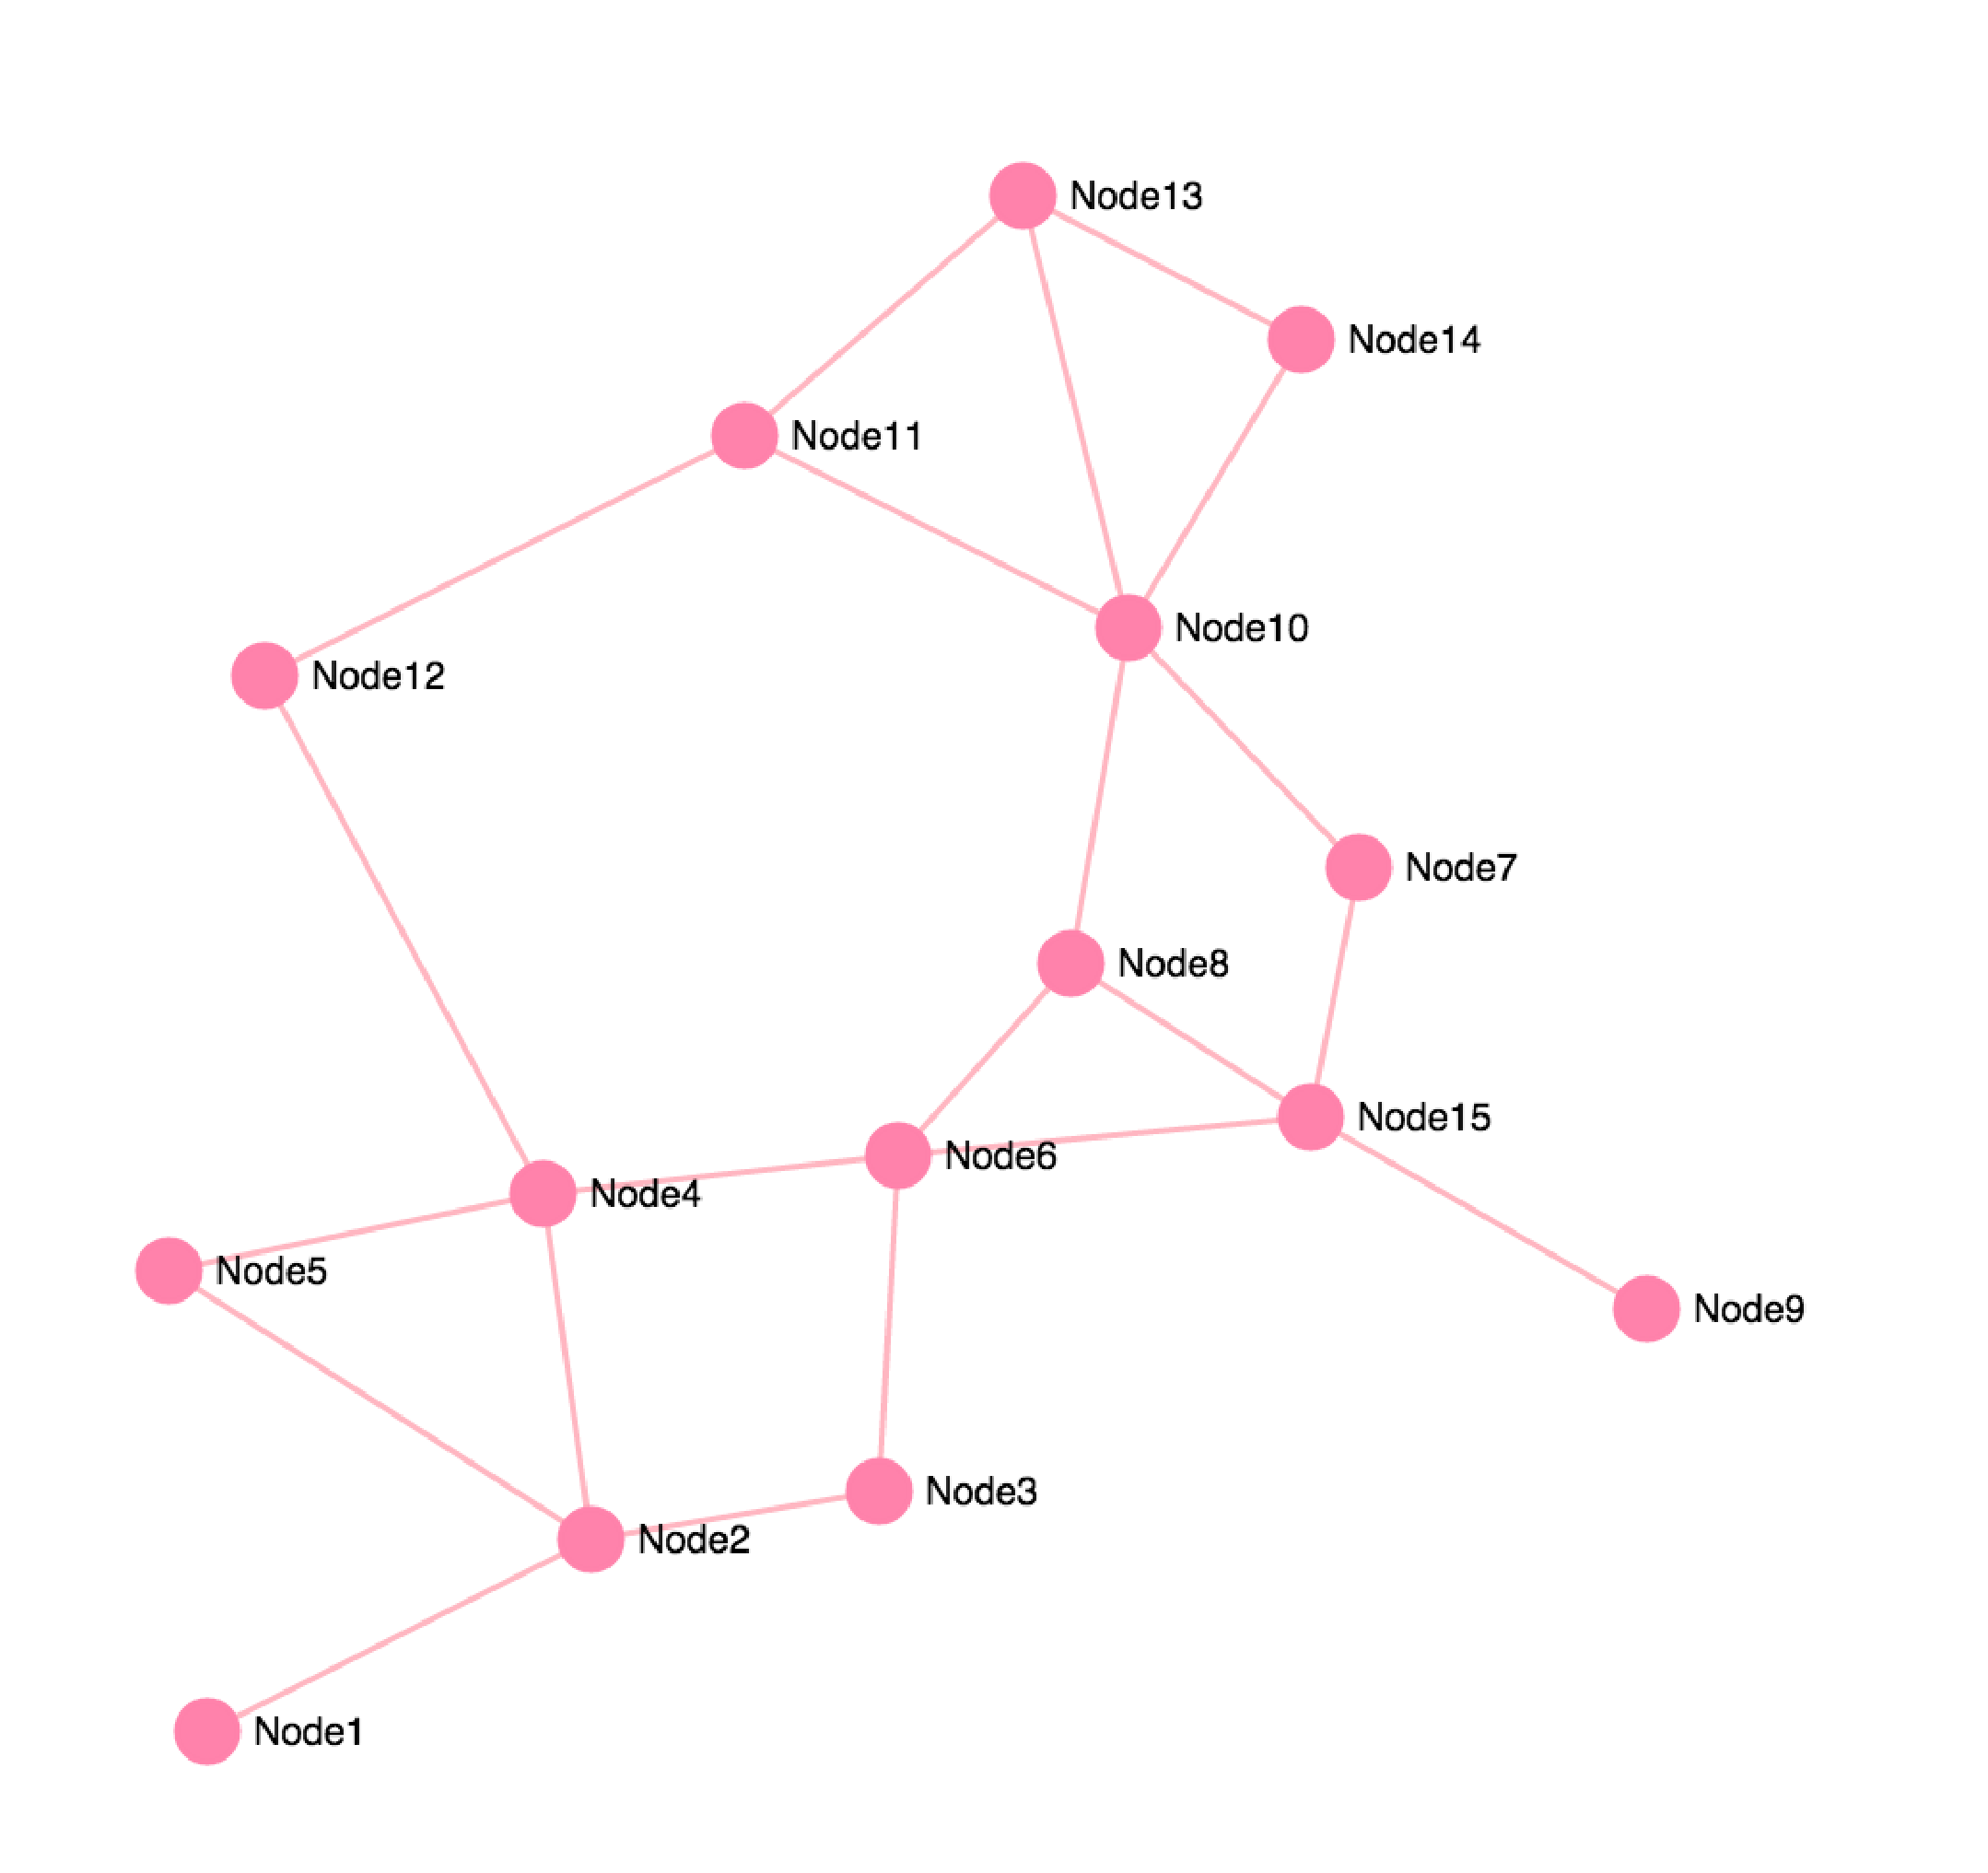
\includegraphics[width=4in]{assets/mandlnetwork_crop.png}
  \end{center}
  \caption{Illustration of Mandl's transit network as a graph}
  \label{fig:MandlNetwork} 
   The transit network including the 15 nodes and 21 edges. The graph is undirected. \emph{\color{red} TODO: Assumptions that it is undirected} Coordinates are correct based on the MandlCoordinates.txt file from \citep{mumford13}
\end{figure}
\chapter{Experimental Results}
\label{appendixC}

\section{Parameter Settings}
%VOL 1 testing:

%SIDEWAYS
%TODO: remove BR and PB
\begin{table}
    \centering
    %\hspace*{-0.5cm}
    \begin{tabular}{|l|l|l|c||c|c|c|c|}
    \hline
    Parameter & $s$ & $i$ & $E$ & $AVG$ & $STD$ & BEST & WORST \\
    \hline
    $s$ & 10$^1$ & 50 & 10\% & 117.244$^1$ $\pm$ 3.854 & 10.700 & 88.364 & 137.997\\
    ~ & 50 & 50 & 10\% & 105.424 $\pm$ 2.369 & 6.619 & 90.076 & 114.843\\
    ~ & 100 & 50 & 10\% & 99.890 $\pm$ 2.193 & 6.128 & 87.178 & 108.688\\
    %~ & 100 & 50 & 0.0 & 99.318 $\pm$ 2.336 & 6.192 & 87.178 & 108.688\\
    ~ & 125 & 50 & 10\% & \textbf{97.994 $\pm$ 2.267} & \textbf{6.334} & \textbf{80.484} & \textbf{105.908}\\
    %~ & 125 & 50 & 0.0 & 99.082 $\pm$ 2.459 & 4.859 & 85.208 & 105.908\\
    \hline
    $i$ & 50 & 10 & 10\% & 113.209 $\pm$ 3.205 & 8.957 & 94.551 & 130.521\\
    ~ & 50 & 50 & 10\% & 105.044 $\pm$ 2.667 & 7.454 & 90.293 & 120.946\\
    ~ & 50 & 100 & 10\% & 101.013 $\pm$ 1.802 & 4.952 & 82.183 & 109.379\\
    %~ & 50 & 100 & 0.0 & 100.855 $\pm$ 1.995 & 5.09 & 82.183 & 109.379\\
    ~ & 50 & 125 & 10\% & \textbf{96.144 $\pm$ 2.106} & \textbf{5.786} & \textbf{82.709} & \textbf{107.362}\\
    %~ & 50 & 125 & 0.0 & 95.241 $\pm$ 2.716 & 6.349 & 82.709 & 107.362\\
    \hline
    $E$ & 50 & 50 & 10\% & 104.395 $\pm$ 2.125 & 5.938 & 92.757 & 115.734\\
    ~ & 50 & 50 & 25\% & \textbf{103.274 $\pm$ 2.998} & \textbf{8.379} & \textbf{86.917} & \textbf{120.811}\\
    ~ & 50 & 50 & 50\% & 103.486 $\pm$ 2.576 & 7.200 & 83.245 & 116.951\\
    ~ & 50 & 50 & 90\% & 104.252 $\pm$ 2.667 & 7.452 & 85.033 & 116.634\\
    \hline
    \end{tabular}
    \caption {Steps with the corresponding results from the parameter settings experiment}
    \tiny
    \begin{itemize}[noitemsep]
    \item[$TOTFIT$ :] Total Fitness function
    \item[$AVG$ :] Average produced $TOTFIT$ with Confidence Interval (confidence level: 95\%)
    \item[$BEST$ :] Best produced result
    \item[$WORST$ :] Worst produced result
    \item[$STD$:] Population Standard Deviation 
    \item[$^1$:] On average 14.467\% of the iterations of each run did not create any ants that satisfied the initial Constraint \ref{itm:criteriaConnectedGraph} described in Section \vref{sec:algoConstraints}.
    \end{itemize}
    \label{table:pm1}
\end{table}

%CA OG FA
\begin{table}
    \centering
    %\hspace*{-0.5cm}
    \begin{tabular}{|l|l|l|c||c|c|c|c|c|}
    \hline
    Parameter & $CA$ & $AF$ & $p_b$ & $AVG$ & $STD$ &BEST & WORST \\
    \hline
    $CA$ & 0\% & 10\% & 0.0 & 105.66 $\pm$ 1.917 & 6.915 & 89.463 & 118.669\\
    ~ & 5\% & 10\% & 0.0 & 104.581 $\pm$ 1.576 & 5.686 & 93.975 & 119.024\\
    ~ & 10\% & 10\% & 0.0 & 104.064 $\pm$ 1.882 & 6.791 & 90.058 & 118.076\\
    ~ & 25\% & 10\% & 0.0 & \textbf{103.597 $\pm$ 2.082} & \textbf{7.511} & \textbf{88.545} & \textbf{119.022}\\
    ~ & 50\% & 10\% & 0.0 & 105.100 $\pm$ 1.726 & 6.228 & 86.434 & 118.981\\
    ~ & 100\% & 10\% & 0.0 & 110.135 $\pm$ 2.26 & 8.153 & 91.194 & 125.927\\
    \hline
    $AF$ & 10\% & 0\% & 0.0 & 105.747 $\pm$ 1.487 & 5.364& 89.031 & 114.771\\
    ~ & 10\% & 5\% & 0.0 & \textbf{104.389 $\pm$ 1.733} & \textbf{6.252}& \textbf{92.358} & \textbf{118.361}\\
    ~ & 10\% & 10\% & 0.0 & 104.739 $\pm$ 1.861 & 6.714 & 91.345 & 123.648\\
    ~ & 10\% & 25\% & 0.0 & 104.632 $\pm$ 1.747 & 6.302 & 87.838 & 118.012\\
    ~ & 10\% & 50\% & 0.0 & 106.327 $\pm$ 2.214 & 7.986 & 89.808 & 119.931\\
    ~ & 10\% & 100\% & 0.0 & 120.245 $\pm$ 3.546 & 12.792 & 94.116 & 145.600\\
    \hline
    $p_b$ & 10\% & 5\% & 0.0 & 104.882 $\pm$ 2.408 & 6.728 & 78.721 & 113.019\\
    ~ & 10\% & 5\% & 0.1 & 103.192 $\pm$ 2.837 & 7.928 & 81.306 & 115.088\\
    ~ & 10\% & 5\% & 0.5 & 104.101 $\pm$ 2.303 & 6.435 &89.282 & 116.23\\
    ~ & 10\% & 5\% & 0.9 & \textbf{102.579 $\pm$ 2.558} & \textbf{7.147} & \textbf{85.033} & \textbf{115.895}\\
    ~ & 10\% & 5\% & 1.3 & 103.058 $\pm$ 1.665 & 4.653 & 92.982 & 111.865\\
    ~ & 10\% & 25\% & 0.0 & 104.861 $\pm$ 2.841 & 7.938 & 88.867 & 117.717\\
    ~ & 10\% & 25\% & 0.1 & 105.613 $\pm$ 2.196 & 6.137 & 95.919 & 120.041\\
    ~ & 10\% & 25\% & 0.5 & 103.646 $\pm$ 3.228 & 9.022 & 79.958 & 116.265\\
    ~ & 10\% & 25\% & 0.9 & 103.682 $\pm$ 2.379 & 6.649 & 91.000 & 115.468\\
    ~ & 10\% & 25\% & 1.3 & 104.228 $\pm$ 2.892 & 8.081 & 89.238 & 117.242\\
    \hline
    \end{tabular}
    \caption {Steps with the corresponding results from the parameter settings experiments (parameter $CA$, $AF$ and $p_b$)}
    \tiny
    \begin{itemize}[noitemsep]
    \item[$TOTFIT$ :] Total Fitness function
    \item[$AVG$ :] Average produced $TOTFIT$ with Confidence Interval (confidence level: 95\%)
    \item[$BEST$ :] Best produced result
    \item[$WORST$ :] Worst produced result
    \item[$STD$:] Population Standard Deviation 
    %\item[$^1$:] On average \% of the iterations of each run did not create any ants that satisfied the initial Constraint \ref{itm:criteriaConnectedGraph} described in Section \vref{sec:algoConstraints}.
    \end{itemize}
    \label{table:pm2}
\end{table}


\section{Performance Comparison}

\begin{table}[H]
    \centering
    \begin{tabular}{|l|llllllll|}
    \hline
    %Route 1: & 1 & 2 & 5 & 4 & 6 & 8 & 10 & 7 \\
    %Route 2: & 1 & 2 & 3 & 6 & 8 & 15 & 7 & 10 \\
    %Route 3: & 12 & 11 & 10 & 14 & 13 &  &  & \\
    %Route 4: & 9 & 15 & 7 & 10 & 11 & 12 & 4 & 2 \\
    \hline
    \end{tabular}
    \caption {Representation of the best route set, having four routes, constructed by ACO}
    \label{table:performanceComparison_bestRouteSet4_ACO}
\end{table}

 %FLyttes til appendix?
    \begin{table}[H]
    \centering
    \begin{tabular}{|l||l|l|l|l|l|}
    \hline
    Algorithm & $d_0(\%)$ & $d_1(\%)$ & $d_2(\%)$ & $d_{unsat}(\%)$ & $ATT$ \\
    \hline
    %ACO Best & 86.16 & 12.59 & 2.25 & 0.00 & 11.16 \\
    %ACO Average & 72.14 & 24.00 & 3.66 & 0.20 & 11.97 \\
    %ACO Median & 72.67 & 23.57 & 3.37 & 0.00 & 11.77 \\
    %ACO Worst & 54.79 & 35.13 & 10.08 & 0.00 & 11.97 \\
    %ACO Standard Deviation & 6.22 & 5.40 & 2.26 & 0.52 & 0.62 \\
    %ACO Relative Standard Deviation & 8.62 & 22.49 & 61.73 & 255.31 & 5.18 \\
    \hline
    \hline
    %SSO Best & 88.44 & 10.28 & 1.29 & 0.00 & 10.67 \\
    %SSO Average & 77.32 & 20.15 & 2.47 & 0.07 & 11.27 \\
    %SSO Median & 77.14 & 20.49 & 2.25 & 0.00 & 11.26 \\
    %SSO Worst & 68.77 & 28.84 & 2.25 & 0.13 & 11.67 \\
    %SSO Standard Deviation & 3.91 & 3.60 & 1.36 & 0.19 & 0.22 \\
    %SSO Relative Standard Deviation & 5.06\% & 17.85\% & 55.16\% & 291.28\% & 1.97\% \\
    \hline
    \end{tabular}
    \caption {Comparing the route sets of ACO and SSO, having four routes, all results}
   % 100 Monte Carlo runs
    \label{table:performanceComparison_ACOFull}
    \end{table}



\end{appendices}


\end{document}